\documentclass[%
candidate,      % тип документа
natbib,         % использовать пакет natbib для "сжатия" цитирований
subf,           % использовать пакет subcaption для вложенной нумерации рисунков
href,           % использовать пакет hyperref для создания гиперссылок
colorlinks=true % цветные гиперссылки
%,times         % шрифт Times как основной
%,fixint=false  % отключить прямые знаки интегралов
%,classified    % гриф секретности
%,libcat        % номер УДК
,facsimile     % отображать факсимиле диссертанта
]{disser}

\usepackage[
  a4paper, mag=1000,
  left=2.5cm, right=1cm, top=2cm, bottom=2cm, headsep=0.7cm, footskip=1cm
]{geometry}
\usepackage[T2A]{fontenc}
\usepackage[utf8]{inputenc}
\usepackage[english,russian]{babel}
%\usepackage{tabularx,longtable}
\ifpdf\usepackage{epstopdf}\fi

\usepackage[ruled]{algorithm}					% Пакеты листингов и алгоритмов
\usepackage[noend]{algpseudocode}
\usepackage{amsthm,amsopn}

% Номера страниц снизу и по центру
%\pagestyle{footcenter}
%\chapterpagestyle{footcenter}

% Точка с запятой в качестве разделителя между номерами цитирований
%\setcitestyle{semicolon}

% Ссылки на работы соискателя включаются в общий список литературы
\let\citemy=\cite

% Использовать полужирное начертание для векторов
\let\vec=\mathbf

% Путь к файлам с иллюстрациями
\graphicspath{{../../images/}}

\DeclareMathOperator*{\argmax}{arg\,max}

\sloppy
\begin{document}

% Переопределение стандартных заголовков
%\def\contentsname{Содержание}
%\def\conclusionname{Выводы}
%\def\bibname{Литература}
\theoremstyle{plain}
\newtheorem{Theorem}{Теорема}
\newtheorem{Def}{Определение}
\newtheorem{Pred}{Утверждение}
\newtheorem{Corollary}{Следствие}
\newenvironment{Proof}%
{
	\par\noindent{\bf Доказательство.}
}%
{
	\hfill$\scriptstyle\blacksquare$
}

\floatname{algorithm}{Алгоритм}
\algrenewcommand\algorithmicrequire{\textbf{Вход:}}
\algrenewcommand\algorithmicensure{\textbf{Выход:}}
\algrenewcommand\algorithmicforall{\textbf{для всех}}
\algrenewcommand\algorithmicwhile{\textbf{пока}}
\algrenewcommand\algorithmicif{\textbf{если}}
\algrenewcommand\algorithmicthen{\textbf{то}}
\algrenewcommand\algorithmicelse{\textbf{иначе}}
\algrenewcommand\algorithmicreturn{\textbf{вернуть}}
\algrenewcommand\algorithmicdo{}
\renewcommand{\algorithmiccomment}[1]{{\quad\sl // #1}}

% Включение файла с общим текстом диссертации и автореферата
% (текст титульного листа и характеристика работы).
% Общие поля титульного листа диссертации и автореферата
\institution{Федеральное государственное учреждение\\
	<<Федеральный исследовательский центр <<Информатика и управление>>
	Российской академии наук>>}

\topic{Методы эффективного решения комбинаторных задач на основе знакового представления знаний}

\author{Панов Александр Игоревич}

\specnum{05.13.17}
\spec{Теоретические основы информатики}
%\specsndnum{01.04.07}
%\specsnd{Физика конденсированного состояния}

\scon{Осипов Геннадий Семенович}
\sconstatus{д.~ф.-м.~н., проф.}
%\sconsnd{ФИО второго консультанта}
%\sconsndstatus{д.~ф.-м.~н., проф.}

\city{Москва}
\date{\number\year}

% Общие разделы автореферата и диссертации
\mkcommonsect{actuality}{Актуальность темы исследования.}{%
Текст об актуальности. Ссылка~\cite{Osipov2002a}.
}

\mkcommonsect{development}{Степень разработанности темы исследования.}{
Текст о степени разработанности темы.
}

\mkcommonsect{objective}{Цели и задачи диссертационной работы:}{%
Список целей.

Для достижения поставленных целей были решены следующие задачи:
}

\mkcommonsect{novelty}{Научная новизна.}{%
Текст о новизне.
}

\mkcommonsect{value}{Теоретическая и практическая значимость.}{%
Результаты, изложенные в диссертации, могут быть использованы для ...
}

\mkcommonsect{methods}{Методология и методы исследования.}{%
Текст о методах исследования.
}

\mkcommonsect{results}{Положения, выносимые на защиту:}{%
Текст о положениях и результатах.
}

\mkcommonsect{approbation}{Степень достоверности и апробация результатов.}{%
Основные результаты диссертации докладывались на следующих конференциях:
}

\mkcommonsect{pub}{Публикации.}{%
Материалы диссертации опубликованы в $N$ печатных работах, из них $n_1$
статей в рецензируемых журналах~\citemy{Panov2014a,Panov2014b,Panov2013a}, $n_2$ статей в
сборниках трудов конференций и $n_3$ тезисов докладов.
}

\mkcommonsect{contrib}{Личный вклад автора.}{%
Содержание диссертации и основные положения, выносимые на защиту, отражают персональный вклад автора в опубликованные работы.
Подготовка к публикации полученных результатов проводилась совместно с соавторами, причем вклад диссертанта был определяющим. Все представленные в диссертации результаты получены лично автором.
}

\mkcommonsect{struct}{Структура и объем диссертации.}{%
Диссертация состоит из введения, обзора литературы, $n$ глав, заключения и библиографии.
Общий объем диссертации $P$ страниц, из них $p_1$ страницы текста, включая $f$ рисунков.
Библиография включает $B$ наименований на $p_2$ страницах.
}

% номер копии для грифа секретности
%\copynum{1}
% класс доступа
%\classlabel{Для служебного пользования}

% номер УДК
\libcatnum{004.81}

\title{ДИССЕРТАЦИЯ\\
на соискание учёной степени\\
кандидата физико-математических наук}

\maketitle

% Содержание
\tableofcontents

% Введение
\chapter*{Введение}							% Заголовок
\addcontentsline{toc}{chapter}{Введение}	% Добавляем его в оглавление
\textbf{Актуальность темы исследования.} 

Исследование картины мира (КМ) субъекта деятельности является одним из центральных направлений в психологии. Высшие психические функции, в том числе когнитивные, познавательные, связанные с приобретением и использованием знаний, являются продуктом работы КМ субъекта в широком смысле. Исследованию большого числа процессов, протекающих в КМ, в~том числе высших, таких как категоризация и обобщение, целеполагание, планирование, принятие решения, творческие синтез и анализ, было посвящено огромное количество работ на протяжении всей истории психологической науки. Следует отметить работы по восприятию Дж.\,А.~Фодора (J.\,A.~Fodor), Б.~Юлеза (B.~Julesz), Дж.\,Е.~Каттинга (J.\,E.~Cutting), А.\,Р.~Лурия, Б.\,М.~Величковского, В.\,П.~Зинченко и памяти С.~Стернберга (S.~Sternberg), Л.~Джакоби (L.~Jacoby), Р.~Аткинсона (R.~Atkinson), Р.~Шиффрина (R.~Shiffrin), Е.~Тулвинга (E.~Tulving).

В последнее время исследованию когнитивных функций человека уделяется большое внимание не только в самой психологии, но и в нейрофизиологии и в~искусственном интеллекте. Нейрофизиологи основной своей задачей ставят поиск нейронного субстрата психических функций. При этом в качестве основного инструмента здесь выступает картирование участков коры головного мозга и отслеживание динамики активности различных участков при выполнении той или иной когнитивной задачи. Большое количество накопленного фактического материала используется для подтверждения целого ряда разрозненных моделей отдельных психических функций. Примерами могут служить работы по моделям внимания Я.\,Б.~Казановича, С.~Фринтропа (S.~Frintrop), С.~Коха (C.~Koch), Л.~Итти (L.~Itti), Дж.\,К.~Сосоза (J.\,K.~Tsotsos), А.~Торралба (A.~Torralba), Л.~Жэнга (L.~Zhang), Р.\,А.~Ренсинка (R.\,A.~Rensink). Единого аппарата для построения таких моделей на данный момент не существует, хотя имеется ряд работ Б.\,Дж.~Баарса (B.\,J.~Baars), Р.~Сана (R.~Sun), Дж.~Хокинса (J.~Hawkins), которые можно считать первыми попытками создания.

Искусственный интеллект в начале своего становления как науки использовал для построения интеллектуальных алгоритмов данные психологов. Однако спустя некоторое время психологические соображения уже перестали рассматриваться как определяющие при разработке того или иного алгоритма. Центральное место стали занимать вопросы вычислительной эффективности и специализации в той или иной предметной области. В~связи с~тем, что в~большинстве интеллектуальных систем в~настоящее время требуется всё большая степень универсальности и автономности, начинается процесс возвращения к психологическим теориям строения психики человека. Возникает задача строить интеллектуальные алгоритмы процессов, например, распознавания и планирования, на некоторой биологически правдоподобной основе. К этому направлению, так называемых биологически обоснованных когнитивных архитектур, относятся работы Дж.\,Р.~Андерсона (J.\,R.~Anderson), П.~Леирда (J.\,E.~Laird), П.~Ленгли (P.~Langley).

Потребность в единой модели КМ субъекта деятельности для нейрофизиологов и исследователей в области искусственного интеллекта определяет актуальность данной работы. Такую модель можно было использовать как для построения моделей когнитивных функций человека на нейронном уровне, подтверждаемых нейрофизиологическими данным о строении нейронных ансамблей и данными об активности соответствующего данной функции участка коры головного мозга, так и для построения абстрагированных от того или иного субстрата интеллектуальных алгоритмов, которые могли бы быть использованы в автономных системах свободной конфигурации.

В работе рассматривается один из основных вопросов, возникающих при разработке модели КМ, посвящённый описанию базовых элементов и построению алгоритма их формирования в процессе деятельности субъекта, носителя КМ. В качестве психологической основы для построения модели элемента КМ был использован культурно"--~исторический подход Л.\,Н.~Выготского и теория деятельности А.\,Н.~Леонтьева. Предпосылки построения таких моделей были заложены а работах Д.\,А.~Поспелова, А.\,М.~Мейстеля, Г.\,С.~Осипова в рамках предложенной ими прикладной семиотики. В качестве нейрофизиологических предпосылок были использованы концепции и нейронные схемы Дж.~Хокинса.

\textbf{Предмет исследования} "--- создание моделей картины мира субъекта деятельности и некоторых высших когнитивных функций.

\textbf{Целью исследования} является разработка моделей и алгоритмов формирования элементов знаковой картины мира субъекта деятельности, обладающих структурой, необходимой для построения моделей высших когнитивных функций, в том числе восприятия, внимания, планирования и целеполагания.

Для~достижения цели работы были поставлены следующие \textbf{задачи}:
\begin{enumerate}
  \item исследовать модель элемента картины мира субъекта, построенную на основе психологической теории деятельности,
  \item построить модель структурных компонент элемента картины мира, опирающуюся на нейрофизиологические данные,
  \item исследовать структуру отношений и процессы самоорганизации на множестве элементов картины мира на синтаксическом уровне,
  \item исследовать итерационный процесс формирования и связывания компонент нового элемента картины мира и разработать соответствующий алгоритм,
  \item исследовать сходимость итерационного процесса формирования и связывания компонент нового элемента картины мира.
\end{enumerate}

\textbf{Научная новизна.}
\begin{enumerate}
	\renewcommand\labelenumi{\theenumi.}
  \item Впервые построена модель структурных компонент элемента картины мира субъекта деятельности.
  \item Построены операторы распознавания в статическом, динамическом и иерархическом случаях в терминах алгебраической теории для образной компоненты элемента картины мира.
  \item Доказаны теоремы корректности линейных замыканий множеств построенных в работе операторов распознавания.
  \item Построен итерационный алгоритм формирования и связывания двух компонент нового элемента картины мира.
  \item Проведено исследование итерационного процесса формирования и связывания компонент нового элемента картины мира.
\end{enumerate}

\textbf{Практическая значимость.} Построение модели картины мира субъекта деятельности, с~одной стороны, позволит создать универсальные интеллектуальные алгоритмы планирования поведения, целеполагания, локализации, распознавания и категоризации, применение которых в интеллектуальных системах повысит степень их автономности, а с~другой стороны, позволит объяснить некоторые патологические явления в мозге человека и дать рекомендации к их преодолению.

\textbf{Методы исследования.} Теоретические результаты работы получены и обоснованы с использованием методов теории множеств, алгебраической теории распознавания образов, теории интеллектуальных динамических систем, теории деятельности.

\textbf{Достоверность результатов} подтверждена строгими математическими доказательствами утверждений и результатами вычислительных экспериментов.

\textbf{Апробация результатов исследования.}

Основные результаты работы докладывались~на: Международных конференциях по когнитивной науке (Томск, 2010~г.; Калининград, 2012~г., 2014~г.), II~Всероссийской научной конференции молодых учёных с международным участием <<Теория и практика системного анализа>> (Рыбинск, 2012~г.), IV~Международной конференции <<Системный анализ и информационные технологии>> (Абзаково, 2011~г.), V~съезде Общероссийской общественной организации <<Российское психологическое общество>> (Москва, 2012~г.), X~Международной конференции <<Интеллектуализация обработки информации>> (Крит, 2014~г.), I~конференции Международной ассоциации когнитивной семиотики (Лунд, 2014~г.), Общемосковском научном семинаре <<Проблемы искусственного интеллекта>>, на семинарах ИСА~РАН.

\textbf{Публикации.} Основные результаты по теме диссертации изложены в 13 печатных работах~\cite{PanovA2011,PanovA2012a,PanovA2012b,PanovA2012c,PanovA2013b,PanovA2014a,PanovT2010b,PanovT2012a,PanovT2012b,PanovT2013,PanovT2014a,PanovT2014b,PanovA2014c,PanovAE2014a}, 3 из которых изданы в рецензируемых журналах из списка ВАК~РФ~\cite{PanovA2012c,PanovA2013b,PanovA2014a}, 7 "--- в материалах всероссийских и международных конференций~\cite{PanovA2011,PanovA2012a,PanovA2012b,PanovT2010b,PanovT2012b,PanovT2014a,PanovT2014b}.

\textbf{Объем и структура работы.} Диссертация состоит из~введения, трёх глав, заключения и~двух приложений. Полный объём диссертации составляет \totalpages\ страниц с \totalfigures\ рисунками\iftotaltables\ и\totaltables\ таблицами\fi. Список литературы содержит \totalcitnums\ наименования.

В \textbf{первой главе} приводится описание предметной области и анализ существующих предпосылок к построению моделей КМ. В~качестве психологических предпосылок рассматриваются культурно-историческое направление в психологии (Л.\,Н.~Выготский и А.\,Р.~Лурия), теория деятельности (А.\,Н.~Леонтьев) и модель психики Е.\,Ю.~Артемьевой. Среди нейрофизиологических моделей наибольшее внимание уделено исследованиям Б.\,Дж.~Баарса и Дж.~Хокинса.

Во \textbf{второй главе} рассматривается синтаксический уровень разрабатываемой модели КМ. Приводится формальное определение знака как элемента картины мира и схема процесса формирования нового знака. Приводится классификация типов отношений, возникающих на множестве знаков, и строятся процессы самоорганизации на сети элементов КМ.

В \textbf{третьей главе} рассматривается семантический уровень разрабатываемой модели КМ. Вводится понятие распознающего блока, являющегося базовым математическим объектом, с помощью которого определяются все компоненты знака. Подробно рассматривается модель процесса восприятия и исследуются множества операторов распознавания, которые строятся при анализе работы образной компоненты знака. Приводится алгоритм итерационного процесса формирования и связывания образа и значения знака, проводится анализ сходимости этого процесса.

В \textbf{приложения} включены описания типов картин мира, свойства которых объясняются с помощью разрабатываемой модели (приложение \ref{AppendixA}) и пример описания одной из когнитивных функций (целеполагания) на синтаксическом уровне (приложение \ref{AppendixB}).

В \textbf{заключении} приводятся основные результаты, полученные в работе.
\clearpage

% Основная часть
%% Глава 1
\chapter{Название главы}
\section{Название секции}
\section{Выводы к первой главе}
%% Глава 2
\chapter{Модель картины мира. Синтаксический уровень} \label{chapt2}

По представлениям психологов \cite{Chudova2012a,Chudova2014} когнитивные функции субъекта, носителя картины мира, работают в двух <<режимах>>: биологическом и культурном. В первом режиме базовой отправной точкой работы психики является сигнал "--- абиотический стимул, используемый субъектом как указатель на определённый биотический стимул, при этом психические функции работают на распознавание биологически значимой ситуации удовлетворения некоторой потребности (физиологической или социальной). Во втором режиме определяющую роль играет знак "--- материальный объект, его свойство или некоторое явление, используемые субъектом как указатель на смысл события, т.\,.е. на собственное желание или желание другого. Знак в этом случае связывает природное и культурное явления, а психические функции работают над задачей понимания сообщения. В данной главе будет рассмотрен внешний, синтаксический уровень модели картины мира, в которой когнитивные функции выполняются именно в знаковом, культурном <<режиме>>.

\section{Знак"--~базовый элемент картины мира} \label{sect2_1}

По А.\,Н.~Леонтьеву \cite{Leontiev1975} представление каждого объекта или процесса в картине мира включает три компоненты: \textit{образ} явления, его \textit{значение} и \textit{личностные смыслы} субъекта, связанные с этим явлением. Для краткости далее вместо словосочетания представление каждого явления в картине мира будет использоваться словосочетание элемент картины мира.

Образ явления представляет собой процедуру обнаружения и отделения этого явления от других, которая реализуется либо низкоуровневыми физиологическими механизмами восприятия, либо высокоуровневыми действиями, требующими специального предварительного акта планирования. Значение представляет собой выработанные в рамках культурно-исторического процесса коллективом, которому принадлежит данный субъект, общепринятые способы использования данного явления в деятельности субъекта, в том числе наборы ситуаций с участием данного явления, в которых принято совершать определённые действия. Наконец, личностный смысл определяет отношение данного явления к той или иной потребности субъекта, которая может быть удовлетворена с помощью набора действий, определяемым самим субъектом на основе своего опыта.

Образ потенциального элемента картины мира, его значение и смыслы могут не связываться в единое целое, и тогда не происходит формирования (в филогенезе) или актуализации (в микрогенезе) знака. В таком случае психическое отражение фиксирует для субъекта не личностный, а \textit{биологический смысл} объекта, не образ мышления, но образ восприятия (\textit{перцепт}), и \textit{функциональное значение} объекта в решаемой задаче вместо значения, выработанного в ходе общественно-исторической практики. Такое внезнаковое отражение реальности позволяет осуществлять лишь <<парные>> переходы между двумя компонентами знания о явлении: 
\begin{itemize}
	\item от перцепта к функциональному значению "--- выбор способа использования конкретного объекта, 
	\item от функционального значения к биологическому смыслу "--- выбор <<цели>> для конкретного действия, 
	\item от биологического смысла к перцепту "--- выбор конкретного объекта, удовлетворяющего заданным критериям.
\end{itemize}
Поскольку три аспекта знания об объекте связаны в этом случае лишь парными зависимостями, то нужен <<внешний наблюдатель>>, чтобы увидеть, что это три компоненты отражения одного явления реального мира \cite{Chudova2012a}.

До момента связывания в знак три компоненты будем называть перцептом, биологическим смыслом и функциональным значением соответственно. Связывание упомянутых трёх компонент в единую структуру позволяет перейти к рассмотрению явления как целостного и существующего независимо от текущего состояния действующего субъекта. Такое связывание становится возможным благодаря именованию возникающей структуры, что приводит к конструкции, называемой \textit{знаком}. При этом знак и его компоненты становятся элементами \textit{языковой системы}, т.\,е. осуществляется включение знака в картину мира субъекта (чего не происходит без именования). Сам объект приобретает при этом устойчивое и общепринятое значение, личный опыт действования с ним отражается в личностном смысле как компоненте знака, а событие восприятия объекта, представляющее собой в простейшем случае отражение в симультанном <<рисунке>> процедуры воспроизведения свойств объекта моторикой воспринимающего органа, фиксируется как образ явления.

%\newpage
%============================================================================================================================

\section{Процесс формирование нового знака} \label{sect2_2}

Следуя \cite{PanovA2014a} приведём схему процесса формирования (актуализации) знака.
\begin{enumerate}
	\setcounter{enumi}{-1}
	\renewcommand\labelenumi{\theenumi.}
	\item\label{step0} Локализация явления. Происходит это в пространстве, в котором наряду с четырьмя измерениями физического пространства"--~времени существует пятое квази"--~измерение "--- измерение значений \cite{Leontiev1983}. При этом субъект определяет положение явления относительно самого себя. Это значит, что он должен реализовывать функцию самосознания (рефлексию), знать свои <<координаты>> в этом пространстве, т.\,е. пребывать, как говорят психиатры, в состоянии ясного сознания (уметь определить не только физические, но и социальные параметры самого себя и ситуации, в которой он оказался).
	\item\label{step1} Формирование перцепта. Основано на работе процедуры воспроизведения свойств явления моторикой воспринимающего органа (для живых существ) или на обработке методами распознавания образов информации, снимаемой с датчиков (для искусственных систем).
	\item\label{step2} Порождение на основе прошлого опыта или на основе прецедентов в виде множества пар <<перцепт "--- функциональное значение>> и сформированного на шаге \ref{step1} перцепта "--- функционального значения явления.
	\item\label{step3} Оценка специальным механизмом степени близости функционального значения, полученного на стадии \ref{step2} к функциональному значению, полученному на стадии \ref{step0}; в случае недостаточной близости "--- переход к шагу \ref{step1} и продолжение формирования перцепта (в психологии сенсорно"--~перцептивных процессов этот механизм получил название <<сенсорная уверенность>>).
	\item\label{step4} Стадии \ref{step1}--\ref{step3} выполняются до получения степени близости, достаточной с точки зрения специального механизма, упомянутого на шаге \ref{step3}.
	\item\label{step5} Получение субъектом из культурной среды, аккумулированной в системе естественного языка, пары <<имя знака "--- значение>> и оценка специальным механизмом степени близости функционального значения, построенного на стадии \ref{step4} к значению, полученному из культурной среды; в случае недостаточной близости "--- переход к шагу \ref{step1} и продолжение формирования перцепта.
	\item\label{step6} Связывание имени из пары <<имя знака "--- значение>> с перцептом, построенным после завершения выполнения шагов \ref{step1}--\ref{step5}. С этого момента перцепт превращается в образ.
	\item Формирование личностных смыслов знака на основе прецедентов действий с явлением.
	\item Связывание имени из пары <<имя знака "--- значение>> со сформированным личностным смыслом. С этого момента функциональное значение превращается в значение, а биологический смысл "--- в личностный смысл.
	\item Продолжение отображения <<биологический смысл "--- перцепт>> включением в область определения отображения личностного смысла, полученного в предыдущем пункте, а в область значений "--- образа из шага \ref{step6}.
\end{enumerate}

В результате образован знак, соответствующий явлению. При этом следует отметить, что в следствие шага \ref{step2} формирование знака вне культурной среды невозможно. Далее будет дано уточнение приведённой схеме.

\subsection{Компоненты знака и процедуры связывания}\label{subsect2_2_1}

Итак, пусть:
\begin{itemize}
	\item $A$ "--- множество смыслов (как личностных, так и биологических),
	\item $M$ "--- множество значений,
	\item $P$ "--- множество признаков объектов.
\end{itemize}

Тогда:
\begin{itemize}
	\item $a\subseteq A$ "--- подмножество множества личностных смыслов (возможно пустое),
	\item $m\subseteq M$ "--- подмножество множества значений (функциональное либо культурно"--~историческое),
	\item $p\subseteq P$ "--- подмножество множества признаков (перцепт либо образ) (Рисунок~\ref{fg:sign}).
\end{itemize}

\begin{figure}[h]
	\centering
	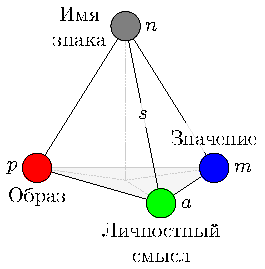
\includegraphics[width=0.5\linewidth]{signs/sign_colored}
	\caption{Знак и его структура.}
	\label{fg:sign}
\end{figure}

Переходы от множества признаков $Р$ к его различным подмножествам реализуются благодаря наличию у субъекта действования встроенных процедур распознавания образов. Процесс формирования знака начинается с работы именно этих процедур. Благодаря им происходит переход от универсального множества свойств $Р$ к его подмножеству, представляющему рассматриваемое явление и отделяющему его от остальных. На первом этапе формирования знака этот процесс приводит к формированию образа восприятия или перцепта. На внутреннем или семантическом уровне построению перцепта соответствует последовательное применение некоторого множества процедур распознавания образов, чему посвящён параграф \ref{sect3_1}.

Что касается значения $m$, то на первом этапе формирования знака подмножества $m$ из $М$ суть функциональные назначения предмета, т.е. способы его использования, далее превращающиеся в значения. Итерационная процедура формирования функционального значения подробно описана в параграфе \ref{sect3_2}.

Подмножество $а$ множества личностных смыслов $А$ возникает благодаря опыту действования с предметом. Всякое подмножество личностных смыслов а будем интерпретировать как множество таких действий с предметом, соответствующим знаку, которые некоторым специальным механизмом оценены как успешные. Этот <<специальный>> механизм есть одна из процедур самосознания и в данной работе подробно не рассматривается. Формирование личностного смысла осуществляется на основе прецедентов.

Введём далее отображения связывания. Заметим, что эти отображения являются частичными функциями из булеанов $P$, $M$ и $A$ в булеаны $M$, $A$ и $P$ соответственно. Наша цель "--- продемонстрировать, каким образом эти отображения строятся субъектом деятельности. Разумеется, будем полагать, что субъект уже обладает минимальным опытом, т.е. ранее выполнял какие-то действия.

Первое из таких отображений $\Psi_p^m:2^P\rightarrow 2^M$ "--- процедура связывания образа (или перцепта) $p$ с (функциональным) значением $m$ так, что $\Psi_p^m(p^{(i)})=m^{(i)}$, где $p^{(i)}\in 2^P$, $m^{(i)}\in 2^M$, $2^P$ и $2^M$ "--- булеаны $P$ и $M$ соответственно.

Второе отображение $\Psi_m^a:2^M\rightarrow 2^A$ связывает значения (или функциональные значения) с личностными (или биологическими) смыслами таким образом, что $\Psi_m^a(m^{(i)})=a^{(i)}$, где $m^{(i)}\in 2^M$, $a^{(i)}\in 2^A$, $2^A$ "--- булеан $A$. Отображение $\Psi_a^p:2^A\rightarrow 2^P$ связывает личностные (или биологические) смыслы с образом (перцептом) так, что $\Psi_a^p(a^{(i)})=p^{(i+1)}$, где $a^{(i)}\in 2^A$, $p^{(i+1)}\in 2^P$.

Все перечисленные выше процедуры являются итерационными (верхние индексы в скобках соответствуют номеру итерации). Действуя на основе приведённой в начале настоящего параграфа схемы рассмотрим стадии формирования знака предмета в микрогенезе или стадии актуализации знака.

\subsection{Формирование функционального значения и образа восприятия} 

Как было сказано выше, считается, что субъект обладает некоторым опытом действования, который зафиксирован, в частности, в прецедентах (примерах) применения отображения $\Psi_p^m:2^P\rightarrow 2^M$. Будем считать, что множество прецедентов есть множество упорядоченных пар вида $\langle p,m\rangle$ таких, что $\Psi_p^m(p^{(i)})=m^{(i)}$, где $p^{(i)}\in 2^P$, $m^{(i)}\in 2^M$.

Применим для описания процесса формирования перцепта и функционального значения элементарные топологические соображения. Заметим, что $(P, T_P)$ и $(M, T_M)$ суть дискретные топологические пространства с топологиями $T_P=2^P$ и $T_M=2^M$ соответственно. Тогда отображение $\Psi_p^m: 2^P\rightarrow 2^M$ есть отображение топологического пространства $(P, T_P)$ в топологическое пространство $(M, T_M)$. Пусть $N=\langle i_1,i_2,\dots,i_n\rangle$ "--- последовательность итераций отображения $\Psi_p^m$ топологического пространства $(P, T_P)$ в топологическое пространство $(M, T_M)$. Тогда бинарное отношение $\geqslant$ является направлением на $N$, а $(\Psi_p^m | N, \geqslant)$ "--- последовательностью по направленному множеству $N$. Поскольку $\Psi_p^m(p^{(i)})=m^{(i)}$, где $m^{(i)}\in (M,T_M)$, то $\Psi_p^m$  "--- направленность в $М$.

Пусть $m$ "--- некоторая точка в пространстве $(M,T_M)$, $\sigma$ "--- система окрестностей точки $m$. В результате применения отображения $\Psi_m^p$ (т.е. отображения, обратного $\Psi_p^m$) возникает некоторый начальный перцепт $p^{(0)}$.

В результате работы механизмов распознавания образов (рассмотрение которых здесь опущено) в $(P,T_P)$ формируется перцепт $p^{(1)}$. Отображение $\Psi_p^m$ ставит ему в соответствие функциональное значение $m^{(1)}$ из $(M,T_M)$.

Далее возможны три случая:
\begin{enumerate}
	\item\label{choise_1} $m^{(1)}=m$,
	\item\label{choise_2} $m^{(1)}\not\in\sigma$,
	\item\label{choise_3} $m^{(1)}\in\sigma$.
\end{enumerate}

Начнём со случая \ref{choise_2}. Для большей определённости допустим, что $p^{(1)}$ "--- одноэлементное множество. Тогда если $m^{(1)}\not\in\sigma$, то следует выбрать, вообще говоря, другое одноэлементное множество $p^{(2)}$ и вновь применить отображение $\Psi_p^m(p^{(2)})=m^{(2)}$. Содержательно это означает, что признак $p^{(1)}$ был выбран неудачно и не являлся существенным. С точки зрения распознавания образов требуется настройка процедур распознавания. Этот процесс продолжается до тех пор, пока не будет получен случай \ref{choise_3}.

В случае \ref{choise_3} имеет место следующее: тогда и только тогда, когда, начиная с некоторого $k$, последовательность $(\Psi_p^m,\geqslant)$ по направленному множеству $(\Psi_p^m | N,\geqslant)$ остается в окрестности $\sigma$ точки $m$, тогда она сходится к точке $m$. Однако топология $(M,T_M)$ является дискретной, в которой любое множество открыто; тогда из того, что $m$ "--- предел последовательности $(\Psi_p^m,\geqslant)$, следует, что $m^{(i)}=m$, начиная с некоторого $k$. Этим исчерпывается и случай \ref{choise_1}. Следовательно, $p^{(i)}={(\Psi_p^m)}^{-1}(m)=\Psi_m^p(m)$.

Далее в соответствие с приведённой схемой субъект получает из внешней культурно"--~исторической среды пару <<имя "--- значение>> "--- $\langle n,m^0\rangle$. Пусть $\sigma^0$ "--- система окрестностей точки $m^0$ в $(M,T_M)$. Тогда вновь следует рассмотреть три случая:
\begin{enumerate}
	\item\label{choise0_1} $m=m^0$,
	\item\label{choise0_2} $m\not\in\sigma^0$,
	\item\label{choise0_3} $m\in\sigma^0$.
\end{enumerate}

Если $m\not\in\sigma^0$, то необходимо вновь применить процедуры распознавания и отображение $\Psi_p^m$ до тех пор, пока не будет получен случай \ref{choise0_3}. Остаётся только использовать приведённые в предыдущем абзаце соображения, заменив $\sigma$ на $\sigma^0$, а $m$ "--- на $m^0$. Завершается эта стадия монотонным продолжением функции $\Psi_p^m$ на множество $\{\langle p^{(i)},m^0\rangle\}$.

\subsection{Именование}

Будем рассматривать процедуру получения из внешней среды пары $\langle n,m\rangle$ как функцию $\mathfrak M(n)$, выдающую по имени $n$ значение $m$. Тогда ${(\Psi_p^m)}^{-1}(\mathfrak M(n))$ есть функция, присваивающая имя $n$ перцепту $p^\prime$. Обозначим ее через $\mathfrak P(n)$. Иначе говоря, $\mathfrak P(n)$ есть функция именования перцепта. С получением имени $n$ перцепт $p^\prime$ превращается в образ $p$. На следующем шаге выполняется именование биологических смыслов и тем самым "--- трансформация их в личностные смыслы.

Множество личностных смыслов, как было замечено выше, формируется на основе опыта действий субъекта деятельности с предметом, соответствующим рассматриваемому знаку, и оценки успешности этих действий с помощью механизмов самосознания. Для определённости будем полагать, что этот опыт зафиксирован в отображении $a=\Psi_m^a(m)$, т\,.е. в виде пары $\langle m,a\rangle$. Тогда функция $\mathfrak A(n)$ именования биологического смысла $a^\prime$ будет иметь следующий вид: $\mathfrak A(n)=\Psi_m^a(\mathfrak M(n))$. Биологический смысл $a^\prime$ становится личностным смыслом $a$ (Рисунок~\ref{fg:sign_naming}). Завершается этот процесс монотонным продолжением функции $\Psi_a^p$ на множество $\{a\}$.

\begin{figure}[h]
	\centering
	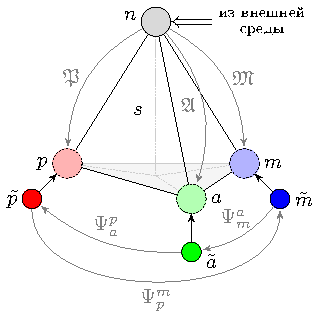
\includegraphics[width=0.5\linewidth]{signs/sign_naming_colored}
	\caption{Процедуры связывания компонент знака и функция именования.}
	\label{fg:sign_naming}
\end{figure}

Легко видеть, что имеют место следующие факты.
\begin{Pred}
	\label{pred:fixed_point}
	Если $s$ "--- знак, $p$, $m$, $a$ "--- его образ, значение и личностный смысл, соответственно, то тройка $\langle p,m,a\rangle$ есть неподвижная точка оператора $\Psi_a^p\Psi_m^a\Psi_p^m$.
\end{Pred}
\begin{Proof}
	Действительно, если $n$ "--- имя знака $s$, то тогда значениями функций именования $\mathfrak P$, $\mathfrak M$ и $\mathfrak A$ в точке $n$ являются соответствующие компоненты знака. В этом случае из определения процедур связывания следует, что $\Psi_p^m(\mathfrak P(n))=\mathfrak M(n)$, $\Psi_m^a(\mathfrak M(n))=\mathfrak A(n)$ и $\Psi_a^p(\mathfrak A(n))=\mathfrak P(n)$. Рассмотрим пространство $Z$, в котором каждая точка $z_i$ представлена тройкой $\langle p_i,m_i,a_i\rangle$. В этом пространстве действие операторов $\Psi_x^y$, $x,y\in\{p,m,a\}$, является поокординатным преобразованием точки, т.е. применение, к примеру, оператора $\Psi_p^m$ к точке $z_i=\langle p_i,m_i,a_i\rangle$ означает преобразование второй координаты таким образом, что в результирующей точке $z'_i=\langle p_i,m'_i,a_i\rangle$ $m'_i=\Psi_p^m(p_i)$. Тогда последовательное покоординатное применение операторов $\Psi_a^p$, $\Psi_m^a$, $\Psi_p^m$ к точке $\langle p,m,a\rangle$, для которой существуют указанные выше функции именования, не приведёт к изменению её координат, т.е. $\Psi_a^p\Psi_m^a\Psi_p^m(\langle p,m,a\rangle)=\langle p,m,a\rangle$, что и требовалось доказать.
\end{Proof}

\begin{Pred}
	Если $s$ "--- знак, то  $\Psi_m^a\Psi_p^m\Psi_a^p$, $\Psi_a^p\Psi_m^a\Psi_p^m$ и $\Psi_p^m\Psi_a^p\Psi_m^a$ "--- тождественные операторы.
\end{Pred}	
\begin{Proof}
	Так как задан знак со своими компонентами, то выполняется условие утверждения \ref{pred:fixed_point} и действие оператора $\Psi_a^p\Psi_m^a\Psi_p^m$ можно записать следующим образом:  $p=\Psi_a^p(a)=\Psi_a^p(\Psi_m^a(m))=\Psi_a^p(\Psi_m^a(\Psi_p^m(p)))$, что и означает тождественность данного оператора. Аналогичным образом выписывается тождественность остальных операторов.
\end{Proof}

\begin{Pred}
	Если $s$ "--- знак, то $\Psi_p^m(\mathfrak P(n))=\mathfrak M(n)$, $\Psi_m^a\Psi_p^m(\mathfrak P(n))=\mathfrak A(n)$.
\end{Pred}	
\begin{Proof}
	Данные тождества следуют из доказательства утверждения \ref{pred:fixed_point}.
\end{Proof}

Подобным образом выписываются ещё шесть фактов такого рода.

%\newpage
%============================================================================================================================

\section{Процедуры самоорганизации} \label{sect2_3}

Рассмотрим структуры, которые могут возникать на множестве знаков как результат их самоорганизации. Моделирование самоорганизации в картине мира позволяет операционализировать представления об <<активности знаний>> \cite{Osipov2002b}, сформировавшееся в искусственном интеллекте под влиянием предложенной Л.~Фестингером в 1956~г. концепции побуждающей роли знаний в поведении человека. Согласно Л.~Фестингеру, знания не просто накапливаются и используются субъектом "--- знания живут своей жизнью, вступают в отношения, образуют то гармоничные, согласованные системы представлений, то оказываются втянуты в конфликты и противопоставляются друг другу. Последний случай, случай рассогласования в знаниях, и выступает как побуждающая поведение сила: <<\dots взгляды и установки имеют свойство объединяться в систему, характеризующуюся согласованностью входящих в неё элементов \dots существование противоречивых отношений между отдельными элементами в системе знаний, само по себе является мотивирующим фактором>> \cite{Festinger1999}.

\subsection{Отношения и операции на множестве образов}\label{subsect_2_3_1}

Пусть $S=\{s_1,s_2,\dots,s_k\}$ "--- множество знаков, $p=(x_1,x_2,\dots,x_g)$ и $q=(y_1,y_2,\dots,y_h)$ "--- образы знаков $s_p$ и $s_q$ соответственно ($p,q\in(2,\dots,k)$).
Пусть $\pi$ "--- множество образов знаков из $S$. Образы $p$ и $q$ из $\pi$ суть множества значений признаков; индексы признаков указывают на их принадлежность тем или иным множествам признаков (доменам); так равенство $i=j$ свидетельствует о принадлежности значений признаков $x_i$ и $y_j$ одному и тому же множеству, например $X_i$.

Упорядоченные множества $\tau_p=\langle i_1,i_2,\dots,i_p\rangle$ и $\tau_q=\langle j_1,j_2,\dots,j_q\rangle$, где $i_1,i_2,\dots,i_p\in(1,\dots,g)$, $j_1,j_2,\dots,j_q\in(1\dots,h$, будем называть типами образов знаков $s_p$ и $s_q$ соответственно.

Введём оператор $Pat$, который для всякого знака $s_p$, просматривает все остальные знаки и выполняет указанные ниже действия (пополняет бинарные отношения).
\begin{enumerate}
	\renewcommand\labelenumi{\theenumi.}
	\item Если для знака $s_p$ и некоторого знака $s_q$ ($p\not =q$) $\tau_p=\tau_q$ и $x_i=y_i$, то $R_1:=R_1\cup\{(p,q)\}$, $R_1\subseteq\pi\times\pi$.
\end{enumerate}
Легко видеть, что отношение $R_1$ является отношением эквивалентности на множестве образов $\pi$. Определённые ниже отношения $R_2$, $R_3$, $R_4$ есть отношения включения, сходства и противопоставления соответственно.
\begin{enumerate}
	\setcounter{enumi}{1}
	\renewcommand\labelenumi{\theenumi.}
	\item Если для знака $s_p$ и некоторого знака $_q$ $\tau_p\subset\tau_q$ и $\forall i\in\tau_p$ имеет место $x_i=y_i$, то $R_2:=R_2\cup\{(p,q)\}$, $R_2\subseteq\pi\times\pi$ (отношение включения).
	\item Если для знака $s_p$ и некоторого знака $s_q$ $\tau_p\cap\tau_q\not =\varnothing$ и $\forall i\in(\tau_p\cap\tau_q)$ имеет место $x_i=y_i$, то $R_3:=R_3\cup\{(p,q)\}$, $R_3\subseteq\pi\times\pi$ (отношение сходства).
	\item Если для знака $s_p$ и некоторого знака $s_q$ $\tau_p\cap\tau_q\not =\varnothing$ и $\forall i\in(\tau_p\cap\tau_q)$ имеет место $x_i\not =y_i$, то $R_4:=R_4\cup\{(p,q)\}$, $R_4\subseteq\pi\times\pi$ (отношение противопоставления).
\end{enumerate}

По существу, приведённые определения суть процедуры порождения новых элементов отношений на множестве знаков. Стартуя всякий раз, когда множество знаков пополняется новым знаком (или когда множество знаков начинает использоваться), описанные процедуры либо формируют новое отношение, либо пополняют какое-либо из отношений на знаках новым элементом. Это означает, что взаимодействие образов различных знаков приводит к формированию на множестве образов неоднородной семантической сети \cite{Osipov1990} с четырьмя типами отношений: эквивалентность образов, включение образов, сходство образов и противопоставление образов.

Рассмотрим в качестве примера операцию обобщения. Частичная операция обобщения $\Theta$ определена на множестве пар образов, принадлежащих отношению $R_3$; результатом работы $\Theta$ является новый образ, включающий все общие признаки исходных образов. Пусть $\pi$ "--- множество образов, $p_1,p_2\in\pi$, $p_1=(x_1,x_2,\dots,x_g)$ и $p_2=(y_1,y_2,\dots,y_h)$, тогда $\Theta:\pi\times\pi\rightarrow\pi$ так, что для всяких $p_1,p_2\in\pi$ таких, что $(p_1,p_2)\in R_3$, $\Theta(p_1,p_2)=p_3$, где $p_3=(z_1,z_2,\dots,z_l)$ так, что для $\forall j\exists j,k$, такие, что $z_i=x_j=y_k$.

Построенный в результате выполнения операции обобщения образ может послужить основой для формирования нового знака. Новый знак образуется аналогично формированию знака, описанному в разд. \ref{sect2_2}, с некоторыми модификациями.
\begin{enumerate}
	\renewcommand\labelenumi{\theenumi.}
	\item Порождение на основе прошлого опыта или на основе прецедентов множества пар вида <<образ "--- значение>> "--- значения знака.
	\item Получение субъектом из культурной среды, аккумулированной в системе естественного языка, пары <<имя знака "--- значение>>.
	\item Связывание имени из пары <<имя знака "--- значение>> с образом.
	\item Формирование личностных смыслов знака на основе прецедентов действий с предметами, описываемыми обобщённым образом.
	\item Связывание имени из пары <<имя знака "--- значение>> со сформированным личностным смыслом.
	\item Продолжение отображения <<личностный смысл "--- образ>> включением в область определения отображения личностного смысла, полученного в предыдущем пункте, а в область значений "--- образа, построенного в п.1.
\end{enumerate}

В результате образуется знак, соответствующий обобщённому образу. При этом пары образов $(р_3,р_1)$ и $(р_3,р_2)$ пополняют отношение включения $R_2$. Новый знак $s_3$ является для знаков $s_1$ и $s_2$ их обобщением по образам (Рисунок~\ref{fg:pattern_gen}).

\begin{figure}[h]
	\centering
	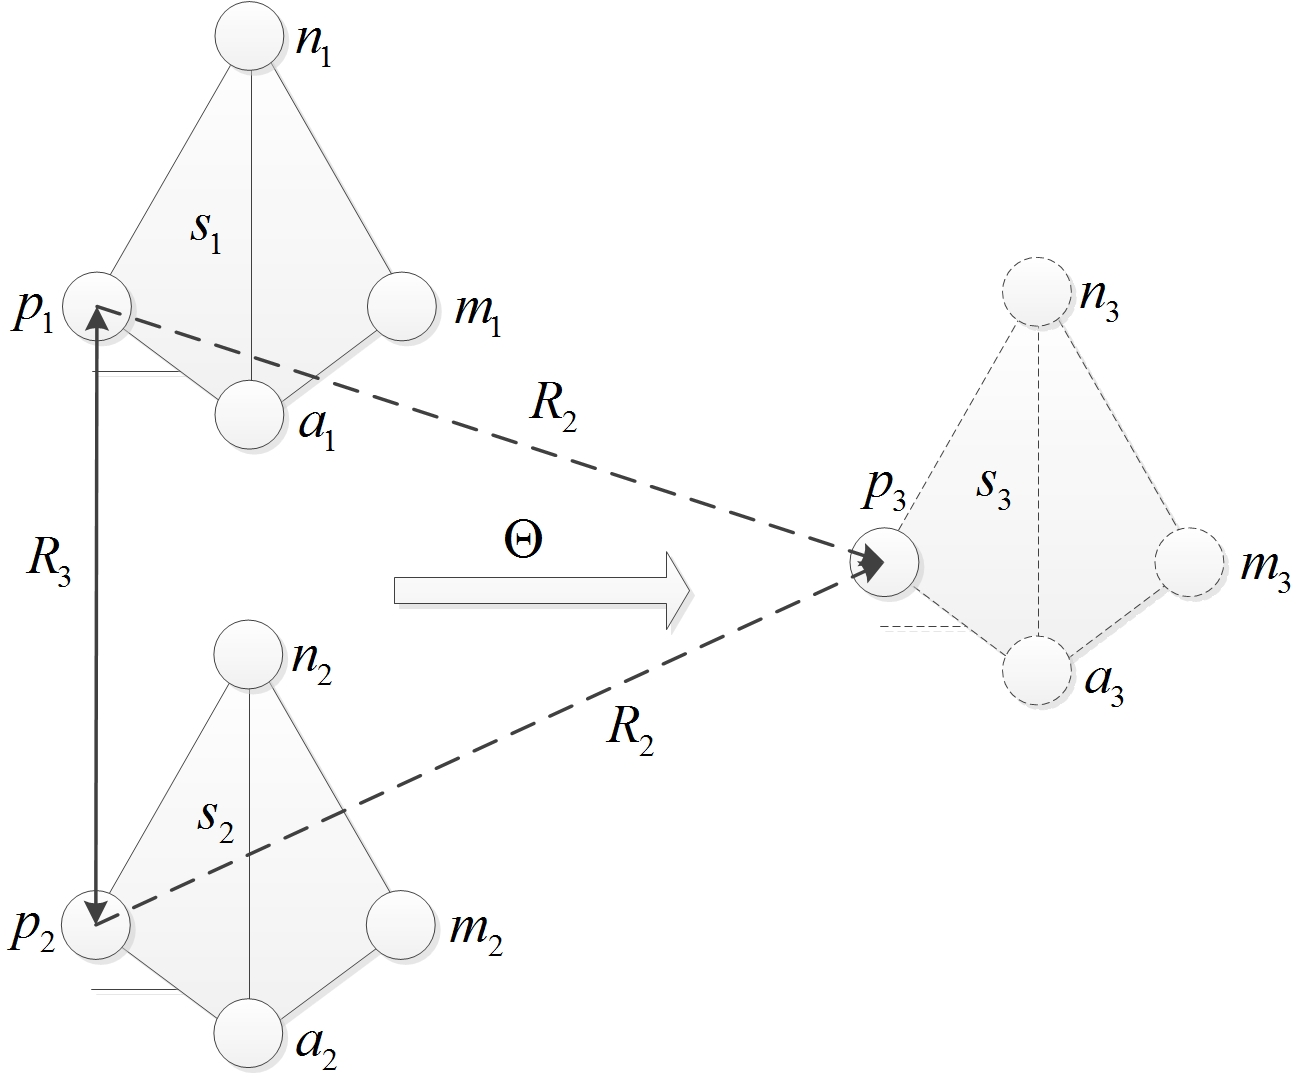
\includegraphics[width=0.7\linewidth]{pattern_gen.jpg}
	\caption{Пример обобщения по признакам. В результате работы операции обобщения $\Theta$ пары знаков $s_1$ и $s_2$, принадлежащих отношению сходства $R_3$, формируется образ $p_3$ нового знака $s_3$ так, что пары $(p_3, p_1)$ и $(p_3, p_2)$ пополняют отношение включения $R_2$.}
	\label{fg:pattern_gen}
\end{figure}

\subsection{Отношения и операции на множестве личностных смыслов}

Как мы видели, с каждым знаком связан некоторый личностный смысл. На множествах личностных смыслов различных знаков оператор $Mean$ естественным образом порождает отношения поглощения, противопоставления и агглютинации (т.е. склеивания, присоединения) смыслов. Определим эти отношения. Пусть по-прежнему $S=\{s_1 s_2,\dots,s_k\}$ "--- множество знаков.

Введём множество действий $ACT$ и функцию $I$, отображающую множество личностных смыслов в булеан $2^{ACT}$ множества действий \cite{Osipov2000}, т.е. функцию, каждому личностному смыслу $a$ из $2^A$ ставящую в соответствие некоторое подмножество $act\in ACT$: $I:2^A\rightarrow 2^{ACT}$ так, что для $\forall а\in 2^A I(а)=act,act\in 2^{ACT}$.

Для всякого знака $s$ отображение $I$ ставит в соответствие каждому личностному смыслу $а$ этого знака множество действий $act$, применимых к объекту, опосредуемому знаком $s$. Эту функцию назовём интерпретацией.

Пусть теперь $I(a_1)=(\alpha_1,\alpha_2,\dots,\alpha_g)$ и $I(a_2)=(\beta_1,\beta_2,\dots,\beta_h)$ "--- интерпретации личностных смыслов знаков $s_1$ и $s_2$. Если действие $\alpha_i$ добавляет некоторый факт \cite{Osipov2000}, а действие $\beta_j$ удаляет тот же факт \cite{Osipov2000}, то будем говорить, что $\alpha_i$ и $\beta_j$ противопоставлены друг другу и принадлежат отношению $R_5:=R_5\cup\{(\alpha_i,\beta_j)\}$, $R5\subseteq AСТ\times AСТ$ "--- отношению оппозиции, т.е. множеству пар действий, образующих оппозиционные шкалы в смысле \cite{Kelly1991}.

Определим следующие отношения на множестве личностных смыслов:
\begin{enumerate}
	\item $\sqsubseteq(a_1,a_2)$ или $a_1\sqsubseteq a_2$ (читается <<смысл $a_2$ поглощает смысл $a_1$>>), если $I(a_1)\subseteq I(a_2)$;
	\item $\perp(a_1,a_2)$  или $a_1\perp a_2$ (<<смысл $a_1$ противопоставлен смыслу $a_2$>>), если $\exists\alpha_1\in a_1,\beta_j\in a_2$, что $(\alpha_i,\beta_j)\in R_5$;
	\item $\sqcup(a_1,a_2,a_3)$ "--- трёхместное отношение агглютинации смыслов, если $I(a_1)\cup I(a_2)=I(a_3)$.
\end{enumerate}

\subsection{Отношения и операции на множестве значений}

Как было сказано выше, значение всякого знака отражает принятые в обществе способы использования соответствующего знаку предмета и поэтому может интерпретироваться некоторым действием. Тогда интерпретация значения напрямую связана с интерпретациями элементов личностного смысла знака. Отметим, что личностный смысл, в отличие от значения, отражает индивидуальные предпочтения субъекта, в то время как значение отражает принятые в обществе способы использования соответствующего знаку предмета. В лексике языка значение, таким образом, может отражаться некоторой группой синонимичных предикатных слов: глаголом, девербативом (т.~е. отглагольным существительным), причастием, деепричастием, которые единственным образом характеризуются своим набором семантических валентностей \cite{Schank1972}.

Пусть $I=\{i_1,i_2,\dots,i_q\}$ "--- множество всех возможных семантических валентностей, тогда каждую группу синонимичных предикатных слов можно характеризовать каким-либо подмножеством этого множества: $I_m=\{j_1,j_2,\dots,j_k\}$, $I_m\subseteq I$. Например, группу предикатных слов движения (<<ехать>>, <<бежать>>, <<идти>>) можно охарактеризовать набором семантических валентностей <<субъект>>, <<средство>>, <<направление движения>>, <<цель>>, <<количественная характеристика>>. 

Пусть $s$ "--- некоторый знак со значением $m$. Экземпляр $\mu$ значения $m$ знака $s$ выражается, в силу сказанного, некоторым предикатным словом и семантической валентностью. Это обстоятельство будем обозначать следующим образом: $\mu(I_m,i)$, где $\mu\in m$ "--- экземпляр значения знака $s$ и $i\in I_m$ "--- семантическая валентность предикатного слова, характеризуемого набором $I_m$. На Рисунке~\ref{fg:mean_scene} приведён пример знака $s$, значение $m$ которого включает два экземпляра: $\mu_1(I_1,i_3)$ и $\mu_2(I_2,j_2)$.

\begin{figure}[h]
	\centering
	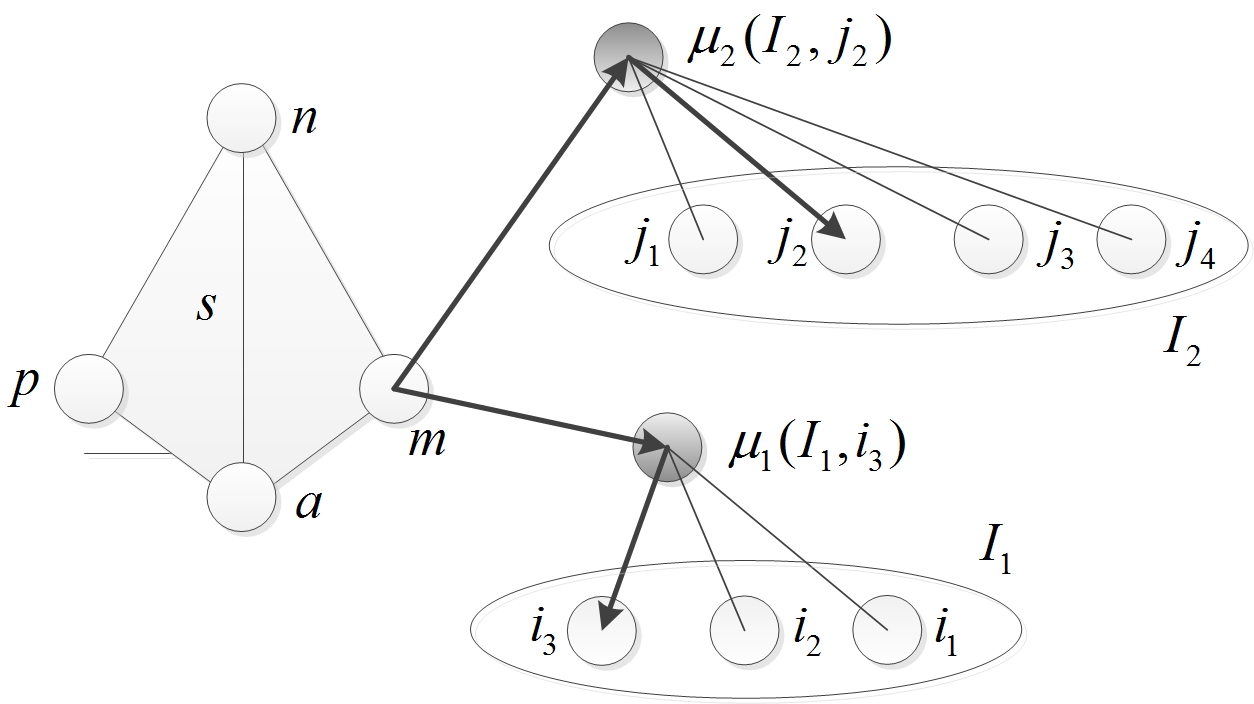
\includegraphics[width=0.7\linewidth]{mean_scene.jpg}
	\caption{Пример структуры значения $m$ знака $s$, которое включает в себя два экземпляра $\mu_1(I_1, i_3)$ и $\mu_2(I_2, j_2)$, где $I_1=\{i_1,i_2,i_3\}$ и $I_2=\{j_1,j_2,j_3,j_4\}$ "--- наборы семантических валентностей.}
	\label{fg:mean_scene}
\end{figure}

Рассмотрим знаки $s_1$ и $s_2$; $\mu_1(I_1,i)$ и $\mu_2(I_2,j)$ "--- экземпляры значений $s_1$ и $s_2$ соответственно. Введём оператор $Des$, который для всякого знака $s_1$ просматривает все остальные знаки и пополняет указанные ниже отношения по следующим правилам.
\begin{enumerate}
	\renewcommand\labelenumi{\theenumi.}
	\item Если $I_1=I_2$ и $i=j$, то $R_1^\prime:=R_2^\prime\cup\{(\mu_1,\mu_2)\}$, $R_2^\prime\subseteq M\times M$.
	\item Если для экземпляра значения $\mu_1$ знака $s_1$ существует экземпляр значения $\mu_2$ знака $s_2$ такое, что $I_1\cap I_2\not =\varnothing$, $I_1\not =I_2$ и $i=j$, то $R_2^\prime:=R_2^\prime\cup\{(\mu_1,\mu_2)\}$, $R_2^\prime\subseteq M\times M$.
	\item Если для экземпляра значения $\mu_1$ знака $s_1$ существует экземпляр значения $\mu_2$ знака $s_2$ такое, что $I_1=I_2$, и $i\not =j$, то $R_6:=R_6\cup\{(\mu_1,\mu_2)\}$, $R_6\subseteq M\times M$ "--- ситуационное отношение.
\end{enumerate}
Аналогично отношениям $R_1$ и $R_3$, отношения $R_1^\prime$ и $R_3^\prime$ являются соответственно отношениями эквивалентности и сходства на множестве значений. 

С каждым экземпляром значения $\mu$ свяжем теперь метку $\tau$, и будем записывать $\mu_1(\tau_1,I_1,i)$ и $\mu_2(\tau_2,I_2,j)$. На множестве меток вводится линейный порядок: для $\forall\tau_1,\tau_2$ справедливо $\tau_1\leqslant\tau_2$ либо $\tau_1\geqslant\tau_2$. Рассмотрим некоторое отношение на $M\times M$. Ограничение этого отношения на $M_{scen}\times M_{scen}$, где $M_{scen}\subseteq M$, будем называть сценарным отношением $R_7$, если оно строится следующим образом.
\begin{enumerate}
	\setcounter{enumi}{3}
	\renewcommand\labelenumi{\theenumi.}
	\item Если $\mu_1\in M_{scen}$, $\mu_2\in M_{scen}$, $I_1\not =I_2$, $i\not =j$ и $\tau_1<\tau_2$, то $R_7:=R_7\cup\{(\mu_1,\mu_2)\}$.
\end{enumerate}	

Элементарным сценарием, порождённым знаком $s$, будем называть множество экземпляров значений $M_{est}(s)$ такое, что для $\forall\mu_1\in M_{est}(s)$ и $\mu_2\in M_{est}(s)$ имеет место:
\begin{itemize}
	\item если $\mu_1\in m$, $\mu_2\in m$ и $\tau_1\geqslant\tau_2$, то $(\mu_1,\mu_2)\in R_7$ (в этом случае сценарное отношение $R_7$ определено на множестве экземпляров значения знака $s$, т.е. $M_{scen}=m$);
	\item если $\mu_1\in m$ и $\mu_2\not\in m$ и $\tau_1\geqslant\tau_2$, то $(\mu_1,\mu_2)\in R_6$.
\end{itemize}

На Рисунке~\ref{fg:mean_relat} приведён пример элементарного сценария $M_{est}(s1)$, порождённого знаком $s_1$, а именно сформированного двумя экземплярами $\mu_2$ и $\mu_3$ значения знака $s_1$ такими, что $(\mu_2,\mu_3)\in R_7$. В примере на Рисунке~\ref{fg:mean_relat} в $M_{est}(s1)$ входят и экземпляры значений $\mu_1$ и $\mu_4$ такие, что $\{(\mu_1,\mu_2),(\mu_3,\mu_4)\}\subseteq R_6$, где $\mu_1$ и $\mu_4$ суть экземпляры значений знаков $s_2$ и $s_3$ соответственно.

\begin{figure}[h]
	\centering
	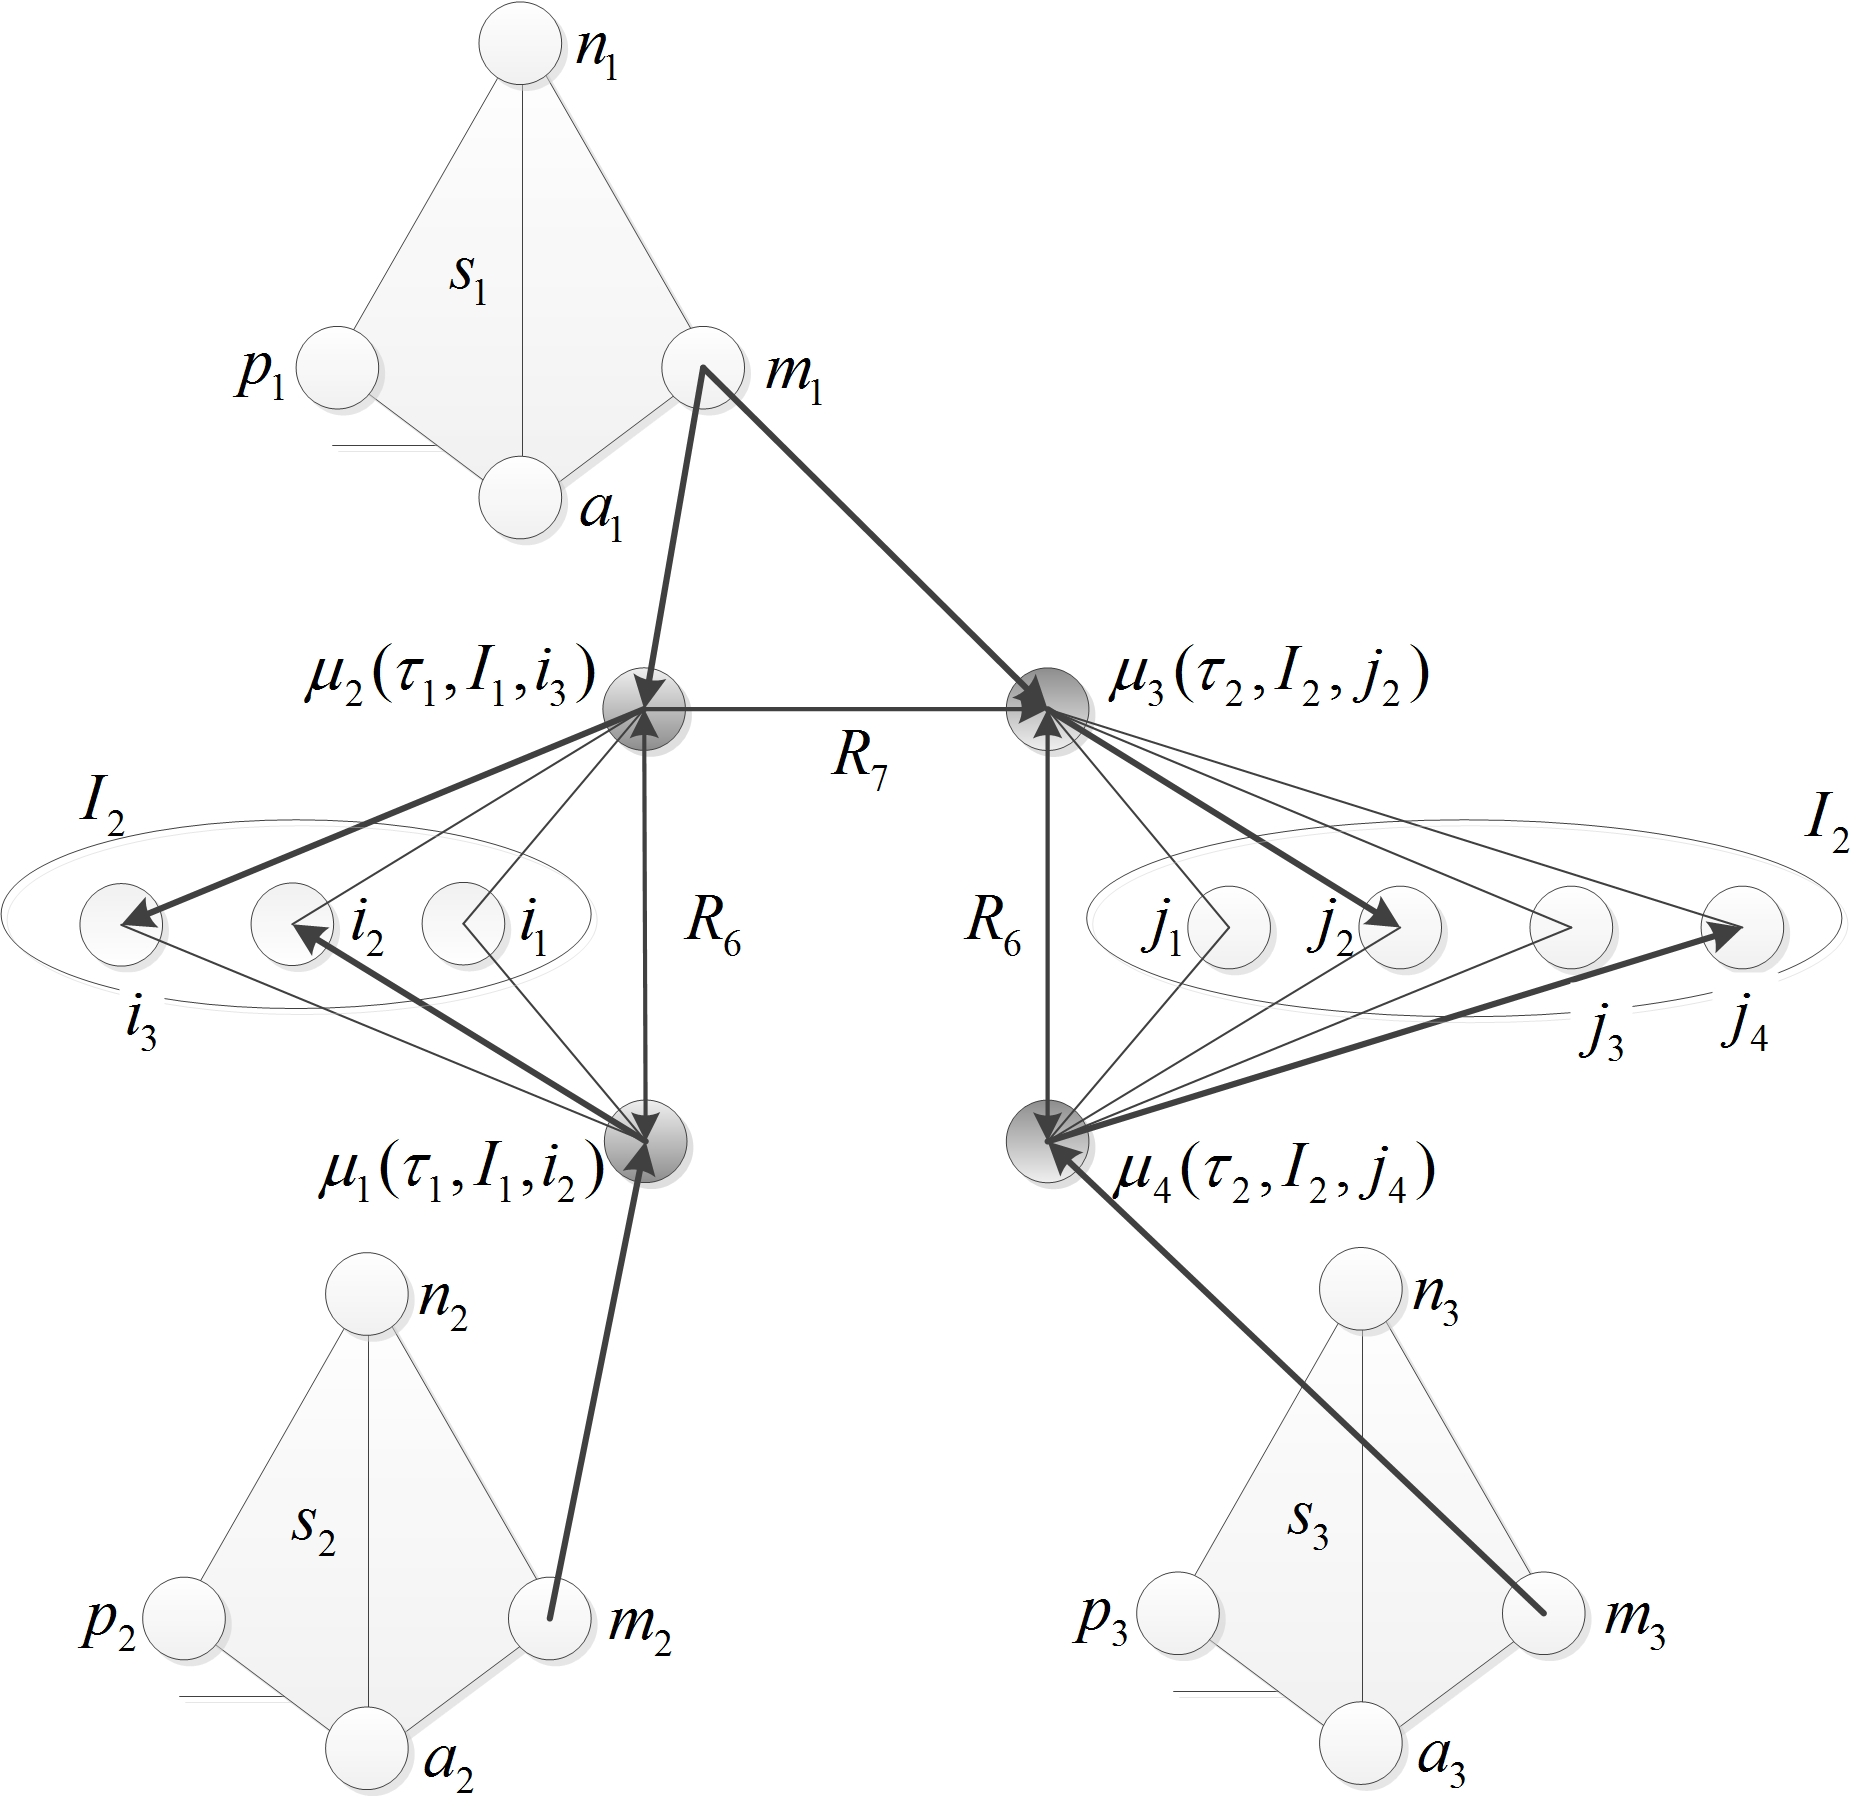
\includegraphics[width=0.7\linewidth]{mean_relat.jpg}
	\caption{Пример элементарного сценария $M_{est}(s_1)=\{\mu_1,\mu_2,\mu_3,\mu_4\}$, порождённого значениями знака $s_1$. Так как в приведённом примере пары экземпляров значений $(\mu_1,\mu_2)$ и $(\mu_3,\mu_4)$ принадлежат отношению $R_6$, а пара $(\mu_1,\mu_3)$ "--- отношению $R_7$, то по определению эти экземпляры принадлежат элементарному сценарию $M_{est}(s_1)$.}
	\label{fg:mean_relat}
\end{figure}

%\newpage
%============================================================================================================================

\clearpage
%% Параграф 3.1
\chapter{Модель картины мира. Семантический уровень} \label{chapt3}

Как было сказано в выводах главы \ref{chapt:review}, внутренний, семантический уровень описания картины мира субъекта деятельности с необходимостью должен быть согласован с нейрофизиологическими данными о строении коры головного мозга человека. В данной главе будет введено такое описание с рядом существенных упрощений, призванных облегчить изложение и позволяющих сконцентрироваться на изучении основных свойств возникающих математических объектов. В начале будет дано семантическое определение образной компоненты и процедуры её функционирования в процессе восприятия, а затем будут введены описания остальных компонент знака, синтаксические определения которых давались в главе \ref{chapt2}. В конце главы дано описание одной из основных функций картины мира "--- процедуры образования нового знака на семантическом уровне и приведены результаты исследования процесса формирования и связывания образа и значения нового знака.

\section{Образная компонента знака}\label{sect3_1}

\subsection{Основные принципы работы образной компоненты} \label{subsect3_1_1}

Далее будем рассматривать модель образной компоненты знака, которая возникают при описании моделей зрительного восприятия, построенных на следующих основных принципах:
\begin{enumerate}
	\item иерархичность,
	\item реализация функции выдвижения перцептивных гипотез,
	\item реализация способности распознавать как динамические так и статические явления,
	\item управляемость.
\end{enumerate}

Эти принципы согласуются с выводами, сделанными при анализе существующей литературы по нейрофизиологическим данным (см. параграф \ref{sect:neuro}). Приведём обоснование выбора именно этих свойств в качестве базовых для построения семантического уровня модели КМ.

Первый принцип был выдвинут в работах когнитивных психологов А. Трисман (A.\,M.~Triesman) и Дж. Джелед (G.~Gelade) \cite{Triesman1980} и заключается в том, что на уровне работы сетчатки имеется набор базовых признаков  или протобъектов (на уровне вторичных зрительных отделов коры головного мозга) \cite{Rensink2000}, из которых в процессе научения образуются более сложные признаки. Из полученных сложных признаков строятся ещё более сложные и т.~д. При этом процесс восприятия представляет собой последовательную активацию части получающейся иерархии, начиная с базовых признаков и заканчивая сложным объектом, предъявляемым зрительной системе. Основным критерием принадлежности разных признаков одному объекту (сложному признаку) является пространственная и временная когерентность. Иерархичность процесса восприятия, как одного из процессов протекающих в картине мира, также проявляется и в функциональной иерархичности коры головного мозга, что подтверждается большим количеством нейрофизиологических данных \cite{Hawkins2009, Bolotova2011}.

Основной задачей образной компоненты на каждом уровне иерархии, таким образом, становится выявление повторяющихся временных и пространственных шаблонов в поступающем наборе сигналов и низкоуровневых признаков.

По данными анализа движения глаз испытуемых доказано, что любой процесс восприятия, как динамического так и статического явления, представляет собой развёрнутый во времени процесс, каждый этап которого с той или иной степенью точности предсказывается на основе предыдущих этапов \cite{Velichkovsky2006, Hawkins2009}. Именно в этом заключается второй принцип: модель элемента картины мира должна включать в себя процессы выдвижения гипотез о том, какая часть иерархии признаков будет активирована в следующий момент времени.

Третий принцип определяет важность параметра времени: образная компонента должна с самого начала уметь работать с меняющимися во времени признаками, не выделяя явно случай статического изображения. Наконец, четвёртый принцип основан на теории активного зрения и том факте, что каждый этап распознавания признака на каком-либо уровне иерархии в процессе восприятия чередуется с активным этапом моторной реакции. Особенно ярко этот факт проявляется в случае зрительного восприятия при наблюдении саккадических движений глаза.

Учитывая перечисленные принципы, на которых строятся большинство существующих моделей восприятия (не только зрительного), в следующем параграфе вводится определение распознающего автомата, являющегося основным структурным элементом как образной, так и других компонент знака (Рисунок~\ref{fg:sign_rb}). Далее приводится алгоритм работы образной компоненты, исследуется его свойства путём постановки ряда задач распознавания.

\begin{figure}[h]
	\centering
    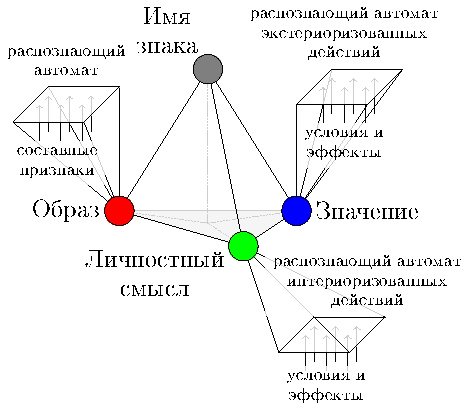
\includegraphics[width=0.7\linewidth]{signs/sign_rb_colored}
    \caption{Знак и его компоненты.}
    \label{fg:sign_rb}
\end{figure}

%============================================================================================================================
\subsection{Распознающий автомат} \label{sect:recogn_block}
Рассмотрим автомат $R_i^j$ вида $<A,Q,B,\varphi,\eta>$ с множествами входов $A$, выходов $B$ и состояний $Q$ и определёнными в соответствии с нейрофизиологическими данными функциями переходов $\varphi$ и выходов $\eta$. Такой автомат будем называть \textit{распознающим автоматом} уровня $j$ с индексом $i$ или просто $R$-автоматом. Опишем кратко его автоматную функцию \cite{Kudryavtcev1985}, а затем определим алгоритм его работы формально.  Для этого воспользуемся понятием \textit{признака}, который будем понимать как составную часть информационного представления некоторой сущности, явления или процесса \cite{Vapnik1974}.

Каждый распознающий автомат распознает или, применительно к~низкоуровневым сигналам, измеряет, некоторые признаки на основе входного вектора данных.  Процесс распознавания (измерения) заключается в сопоставлении признака числу, которое определяет оценку успешности построения (измерения) признака из составляющих его входных признаков, информация о которых содержится во входном векторе. Такое число будем называть \textit{весом признака}.

Входной вектор, в свою очередь, представляет собой вектор весов признаков предыдущего уровня иерархии, по которым распознаются выходные признаки. Распознающий автомат обладает множеством состояний, каждое из которых представляет собой набор бинарных матриц, каждый столбец которых задаёт ожидание входных признаков в следующий момент времени. Такие матрицы будем называть \textit{матрицами предсказаний}. Опишем сказанное более строго.

Пусть заданы множества $\mathcal R$ и $\mathcal F$. Множество $\mathcal R$ будем называть совокупностью распознающих автоматов, а множество $\mathcal F$ "--- совокупностью допустимых признаков. Введём бинарное отношение $\dashv$, определённое на паре множеств $\mathcal F$ и $\mathcal R$, и будем читать $f_k\dashv R_i^j$, $f_k\in\mathcal F$, как <<признак $f_k$ распознаётся $R$-автоматом $R_i^j$>> или как <<признак $f_k$ измеряется $R$-автоматом $R_i^j$>>. Множество всех распознаваемых $R$-автоматом $R_i^j$ признаков будем обозначать $F_i^{*j}$, т.е. ${\forall}f^*{\in}F_i^{*j} f^*{\dashv}R_i^j, F_i^{*j}{\subseteq}\mathcal F$.

Рассмотрим связный ориентированный (ярусный) граф $G_R=(V,E)$, где $V=\mathcal R$ "--- множество вершин, $E\subset \mathcal R\times \mathcal R$ "--- множество рёбер. Каждая вершина $v$, принадлежащую $j$-ому ярусу графа $G_R$, является распознающим автоматом $R_{i_1}^{j_1}$ уровня $j_1$, а ребро $e=(R_{i_1}^{j_1},R_{i_2}^{j_2}){\in}E$ обозначает  иерархическую связь между $R$-автоматом $R_{i_1}^{j_1}$ и $R$-автоматом $R_{i_2}^{j_2}$. $R$-автомат $R_{i_1}^{j_1 }$ в данном случае будем называть дочерним, а $R$-автомат $R_{i_2}^{j_2}$ "--- родительским (Рисунок~\ref{fg:rb_hier}).

\begin{figure}[h]
	\centering
	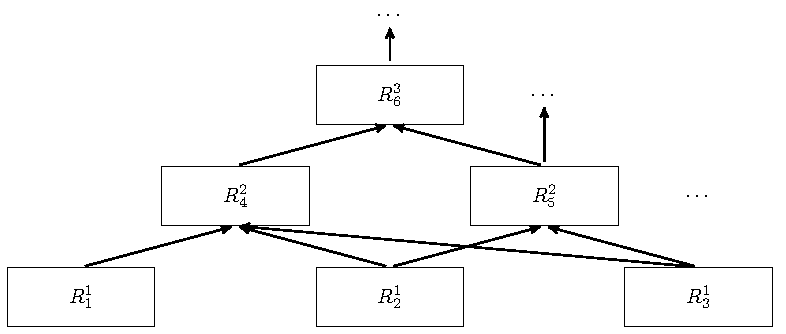
\includegraphics[width=0.7\linewidth]{automata/rb_hierarchy}
	\caption{Пример иерархии распознающих автоматов. Так, узел $R_{i_2}^{j_2}$ является родительским распознающим автоматом, а узел $R_{i_1}^{j_1}$ "--- дочерним автоматом.}
	\label{fg:rb_hier}
\end{figure}

Рассмотрим распознающий автомат $R_i^j$. Определим множество $F_i^j{\subseteq}\mathcal F$ таких признаков, что для любого $f{\in}F_i^j$ существует распознающий автомат $R_k^{j-1}$ уровня $j-1$, дочерний по отношению к $R$-автомату $R_i^j$, такой, что $f{\dashv}R_k^{j-1}$. Такое множество $F_i^j$ будем называть совокупностью входных признаков распознающего автомата $R_i^j$. Некоторые части векторов весов выходных признаков распознающих автоматов $R_{i_1}^j,R_{i_2}^j,\dots,R_{i_q}^j$ путём конкатенации составляют вектор весов входных признаков для родительского автомата $R_k^{j+1}$ следующего уровня иерархии.

Для каждого признака $f^*{\in}F_i^{*j}$ введём функцию распознавания $\hat f:X\rightarrow\mathbb R$, $\hat{f}(x_1,\dots,x_q )=x^*$, где $x^*{\in}[0,1]$ "--- вес распознаваемого признака $f^*$ в выходном векторе, а $x_1,\dots,x_q{\in}[0,1]$ "--- веса признаков из множества $F_i^j$ в текущем входном векторе. Множество таких функций для распознающего автомата $R_i^j$ обозначим как $\hat{F}_i^j$.

Пусть мощность множества распознаваемых признаков $F_i^{*j}$ и множества функций распознавания $\hat{F}_i^j$ равна $l_i^j$, а мощность множества входных признаков $F_i^j$ равна $q_i^j$. Введём упорядоченное множество локальных моментов времени $T_i^j$ для распознающего автомата $R_i^j$. Будем называть \textit{вычислительным циклом} полуинтервал между соседними моментами времени поступления сигналов обратной связи с верхнего уровня иерархии (см. ниже). Для каждого распознающего автомата определим характерное время $h_i^j$, за которое выполняется один цикл вычисления. 

В начале $s$-ого цикла вычисления (момент времени $\tau_s\in{T_i^j}$)  распознающий автомат $R_i^j$ получает на вход вектор длины $l_i^j$ ожиданий $\hat{x}_i^{j+1}(\tau_s)$, вычисляемый по формуле среднего от векторов ожиданий, поступающих от родительских относительно $R$-автомата $R_i^j$ распознающих автоматов $R_k^{j+1}$:
\begin{equation}
	\hat{x}_i^{j+1}(\tau_s)=\frac{1}{N_i^j}\sum_{k{\in}K_i^{j+1}}\hat{x}_k^{j+1}(\tau_s),
\end{equation}
где $N_i^j$ - количество родительских $R$-автоматов, $K_i^{j+1}$ - множество индексов родительских относительно $R_i^j$ распознающих автоматов. Далее в~каждый момент времени $t\in{T_i^j}$, $\tau_s\leqslant{t}\leqslant\tau_s+h_i^j$,  распознающий автомат $R_i^j$ получает на~вход вектор весов $\bar{x}_i^j(t)$ входных признаков из~множества $F_i^j$ длины $l_i^j$, вычисляет выходной вектор весов $\bar{x}_i^{*j}(t)$ распознаваемых признаков из~множества $F_i^{*j}$ длины $l_i^j$, вычисляет вектор ожиданий $\hat{x}_i^j(t)$ входных признаков в следующий момент времени длины $q_i^j$ (Рисунок~\ref{fig:rb_cycle}). Параметр $h_i^j$ , таким образом, служит характеристикой глубины памяти $R$-автомата.
	
\begin{figure}[h]
	\centering
	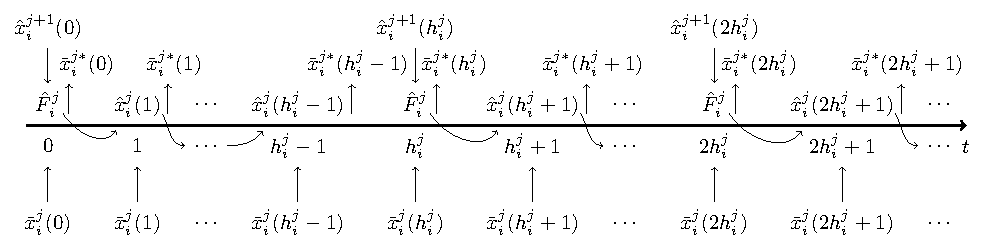
\includegraphics[width=1.0\linewidth]{automata/rb_cycle}
	\caption{Вычислительные циклы распознающего автомата. В моменты времени $0,h_i^j,2h_i^j,\dots$ происходит определение нового начального состояния.}
	\label{fig:rb_cycle}  
\end{figure}

\subsection{Алгоритм $\mathfrak A_{th}$ работы распознающего автомата}\label{subsect:rb_algorithm}

Будем рассматривать распознающий автомат $R_i^j$ как автомат с конечным множеством состояний. Для этого каждой функции распознавания $\hat{f}_k$ из множества $\hat{F}_i^j$ будем ставить в соответствие набор \textit{матриц предсказания} $Z_k=\{Z_1^k,…,Z_m^k\}$ размерности $q_i^j\times h_i^j$, где $h_i^j$ "--- характерное время распознающего автомата $R_i^j$. Столбец $\bar{z}_u^r=(z_{u1}^k,…,z_{uq}^k)$ матрицы $Z_r^k$ интерпретируется как вектор предсказания присутствия входных признаков из множества $F_i^j$ в момент времени $\tau_s+u$, при этом $z_{uv}^k\in\{0,1\}$, т.е. вектор $\bar{z}_u^r$ является булевым вектором. Сама матрица $Z_r^k$ задаёт, таким образом, последовательность событий, наличие которых свидетельствует о~присутствии распознаваемого функцией $\hat{f}_k$ признака. Множество всех матриц предсказания распознающего автомата $R_i^j$ будем обозначать как $\mathcal{Z}_i^j$.

Таким образом, $R$-автомат $R_i^j$ является бесконечным автоматом Мили с переменной структурой и конечной памятью и определяется следующим набором $R_i^j=<X_i^j\times \hat{X}_i^{j+1}, 2^{\mathcal Z_i^j}, X_i^{*j}\times \hat{X}_i^j,\varphi_i^j,\vec\eta_i^j,>$, где
\begin{itemize}
	\item $X_i^j$ "--- множество входных сигналов (пространство векторов длины $q_i^j$ действительных чисел от $0$ до $1$), 
	\item $X_i^{*j}$ "--- множество выходных сигналов (пространство векторов длины $l_i^j$ действительных чисел от $0$ до $1$), 
	\item $\hat{X}_i^{j+1}$ "--- множество управляющих сигналов с верхнего уровня иерархии (пространство векторов длины $l_i^j$ действительных чисел от $0$ до $1$),
	\item $\hat{X}_i^j$ "--- множество управляющих сигналов на нижний уровень иерархии (пространство векторов длины $q_i^j$ действительных чисел от $0$ до $1$),
	\item $2^{\mathcal Z_i^j}$ "--- множество состояний (множество подмножеств множества матриц предсказания),
	\item $\varphi_i^j:X_i^j\times \hat{X}_i^{j+1}\to 2^{\mathcal Z_i^j}$ "--- функция переходов,
	\item $\vec\eta_i^j:2^{\mathcal Z_i^j} \to X_i^{*j}\times \hat{X}_i^j$ "--- вектор"--~функция выходов.
\end{itemize}

Для удобства определения автоматной функции обозначим \textit{входное воздействие} через $\omega_i^j:T{\to}X_i^j$, а \textit{выходную величину} через $\gamma_i^j:T{\to}X_i^{*j}$ как это принято в~теории динамических систем \cite{Kalman1971} (Рисунок~\ref{fig:rb_io}).

\begin{figure}[h]
	\centering
	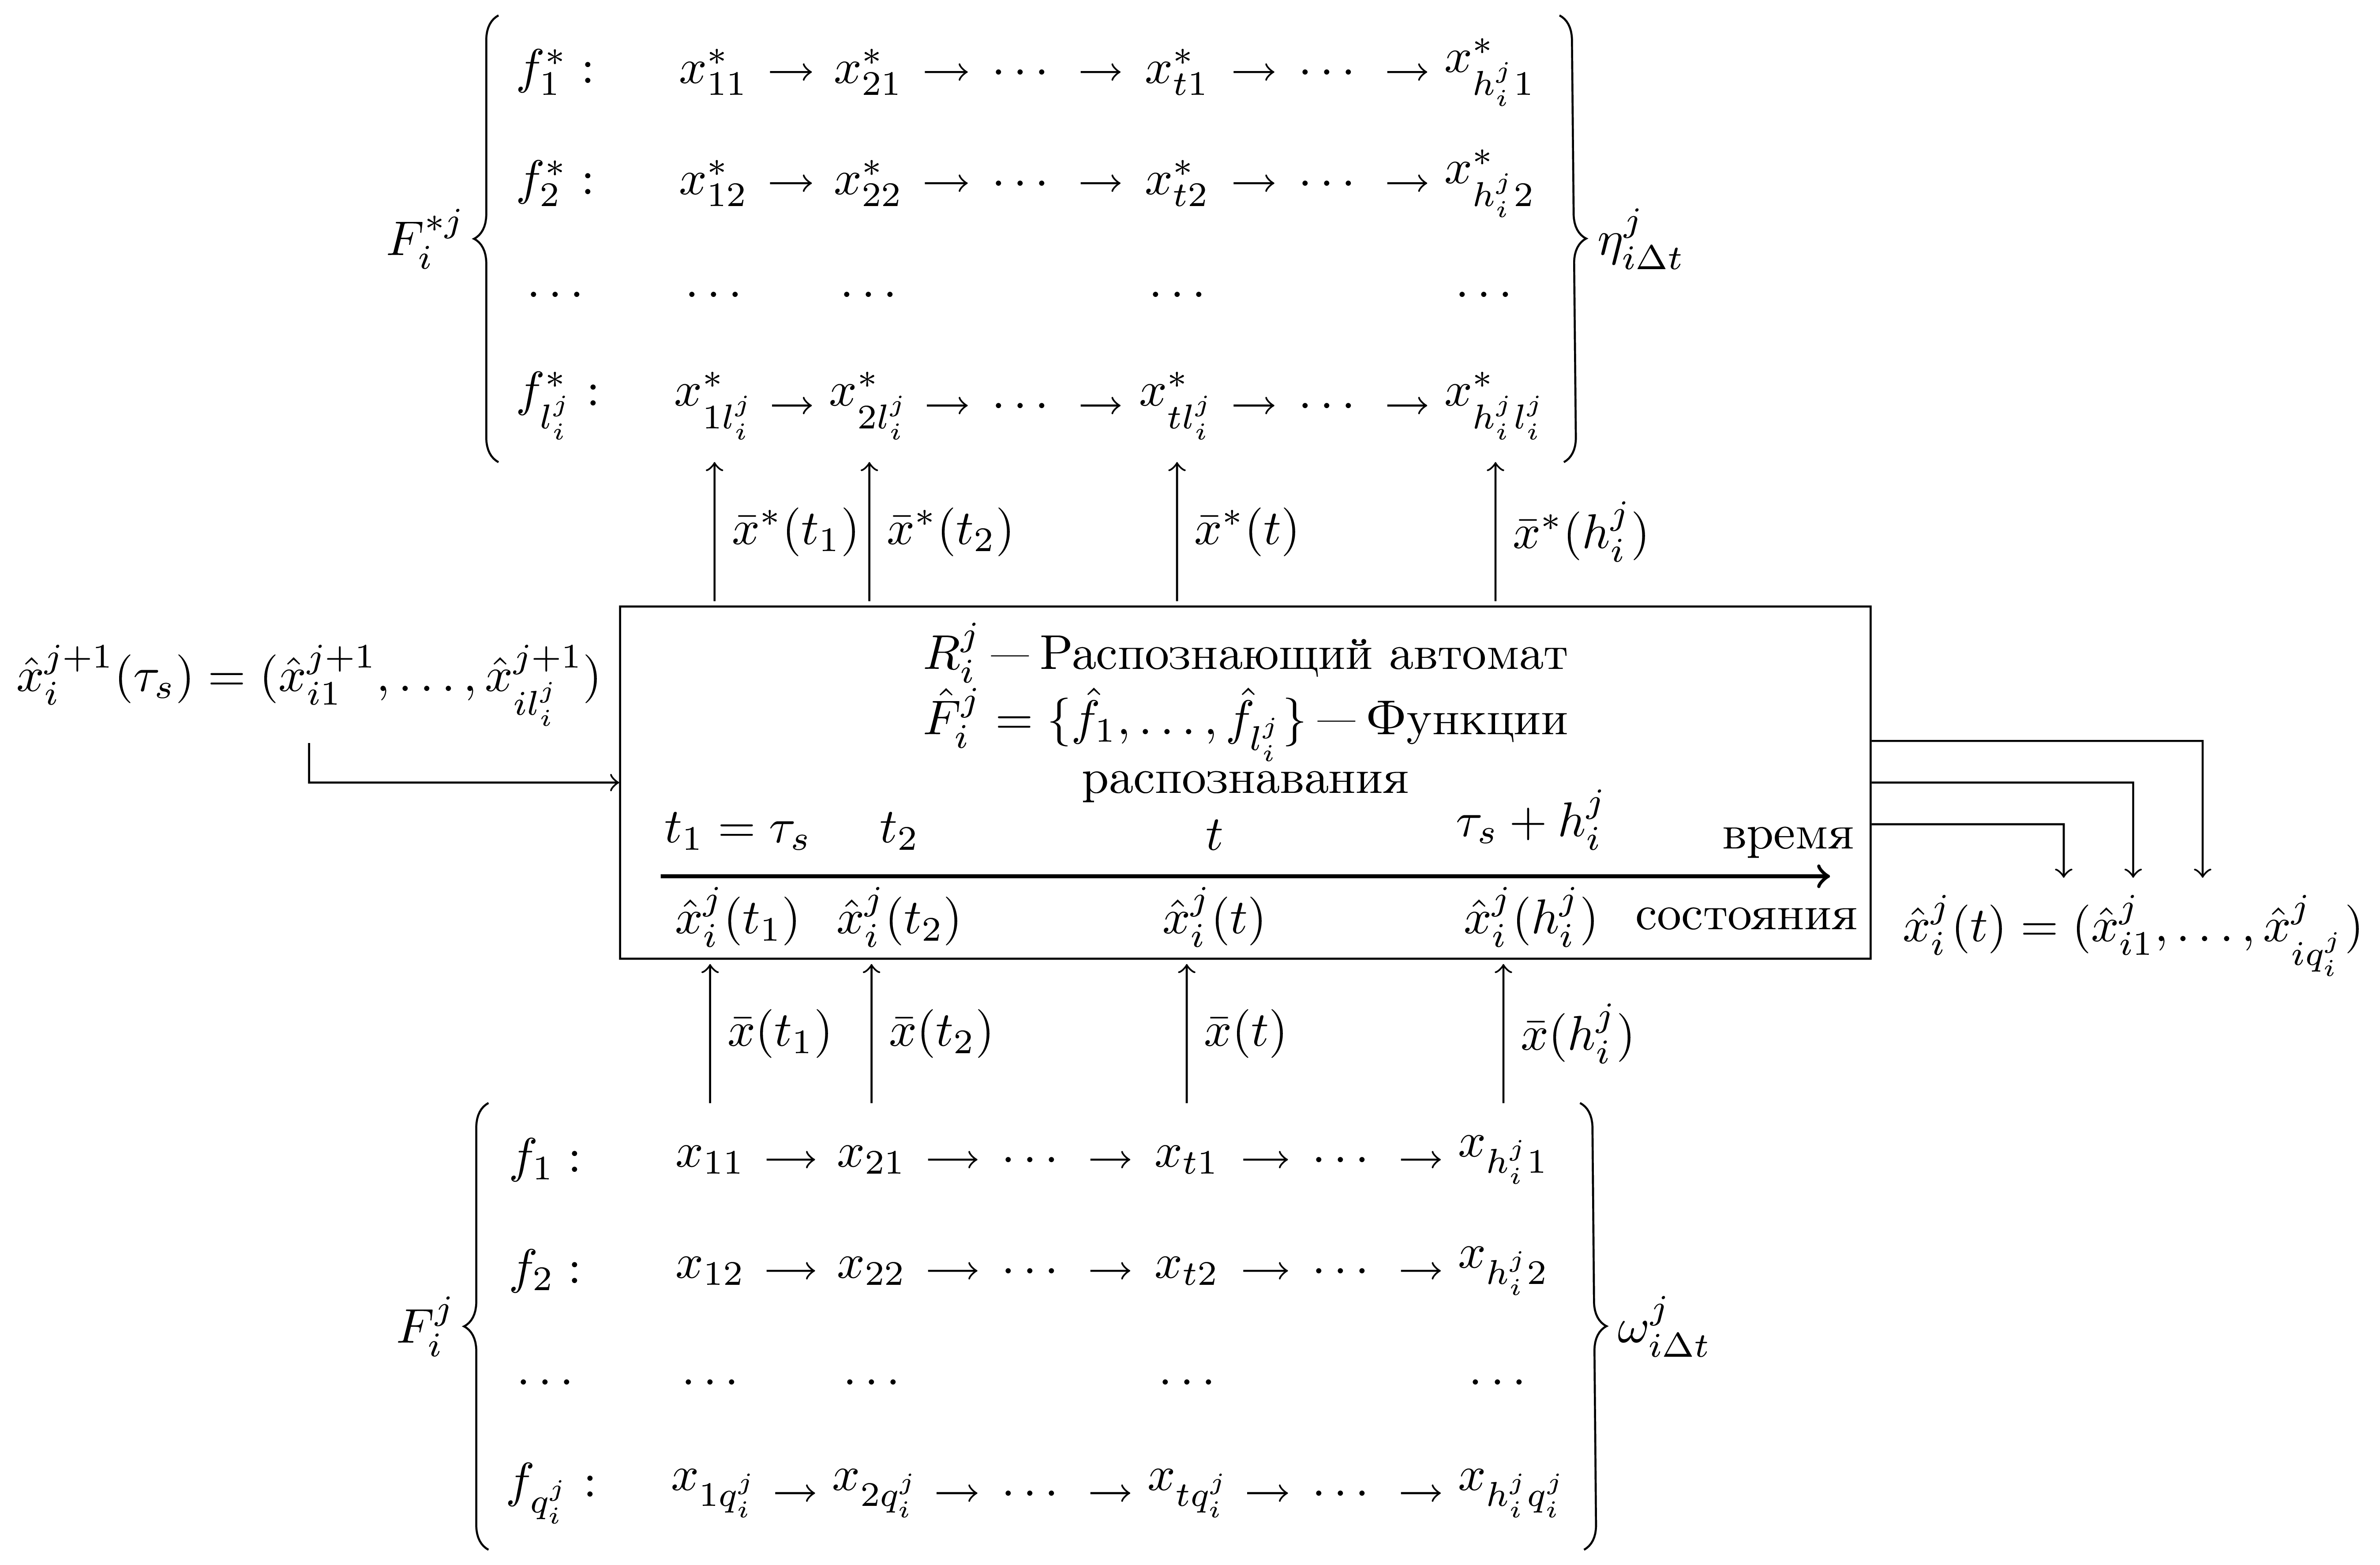
\includegraphics[width=\linewidth]{automata/rb_io}
	\caption{Схема входных и выходных отображений распознающего автомата.}
	\label{fig:rb_io}
\end{figure}

На страницах \pageref{alg:th_init} и \pageref{alg:th_cycle} приведён алгоритм $\mathfrak{A}_{th}$ вычислительного цикла распознающего $R$-автомата, в котором рассчитываются значения функции переходов $\varphi_i^j(\hat{x}_i^{j+1}(\tau_s+t),\omega_i^j)$, $1\leqslant{t}\leqslant h_i^j-1$, и выходной функции $\vec\eta_i^j(\mathcal Z_i^{*j}(\tau_s+t))$, $1\leqslant{t}\leqslant h_i^j-1$, $\mathcal Z_i^{*j}(\tau_s+t)$ "--- текущее состояние. В алгоритме используется функция $W$ нормировки весовых значений:
\begin{equation}
	W(\bar x)=\left(\frac{x_1}{\max\limits_i x_i},\dots,\frac{x_n}{\max\limits_i x_i}\right),
\end{equation} 
где $\bar x=(x_1,\dots,x_n)$ "--- вектор с ненормированными компонентами. Кратко опишем шаги алгоритма.

Вычислительный цикл распознающего автомата начинается с определения начального состояния при~помощи управляющего воздействия с верхних уровней иерархии "--- вектора ожиданий $\hat x_i^{j+1}(\tau_s)$ (шаги \ref{alst:init_start}--\ref{alst:init_end}). Начальное состояние определяется как подмножество таких распознаваемых признаков множества $F_i^{*j}$, которые предсказываются на основе состояния $R$-автоматов верхнего уровня. Первая константа $c_1$ определяет порог предсказываемого веса распознаваемых признаков, выше которого соответствующие функции распознавания попадают во множество активных функций $\hat F^*$ (шаг \ref{alst:select_f}). Далее производится отбор тех матриц предсказания активных функций распознавания, для которых обычное расстояние по норме $\|x\|=\sum_i |x_i|$ первого столбца $\bar z_1^r$ от входного вектора $\bar x_i^j$ в начальный момент времени не превышает второй константы $c_2$ (шаг \ref{alst:select_z}). Множество полученных таким образом активных матриц предсказания и является текущим состоянием распознающего автомата (шаг \ref{alst:init_state}). На основе активных матриц предсказания методом голосования вычисляется выходной вектор в начальный момент времени $\bar x_i^{j*}(\tau_s)$ (шаги \ref{alst:init_calc_out2} -- \ref{alst:init_calc_out3}).

\begin{algorithm}[h]
	\caption{Алгоритм $\mathfrak{A}_{th}$ (часть I, задание начального состояния)}\label{alg:th_init}
	\begin{algorithmic}[1]
				\Require $\tau_s, \hat{x}_i^{j+1}(\tau_s), \omega_i^j$.
		\Ensure $\varphi_{i\Delta t}^j, \vec\eta_{i\Delta t}^j$.

		\State $\hat{F}^*=\varnothing,Z^*=\varnothing,t=0$; \Comment{активные функции распознавнаия и матрицы предсказания}
		\State $c_1\in(0,1), c_2\in(0,1)$; \Comment{пороговые константы}

		\Statex \Comment{определение начального состояния}
				
		\ForAll{компонент $\hat{x}_{ik}^{j+1}$ вектора $\hat{x}_i^{j+1}(\tau_s)=(\hat{x}_{i1}^{j+1},\hat{x}_{i2}^{j+1},\dots,\hat{x}_{il}^{j+1})$} \label{alst:init_start}
			\If{$\hat{x}_{ik}^{j+1}{\ge}c_1$} \label{alst:select_f}
				\State $\hat{F}^*:=\hat{F}^*\cup\{\hat{f}_k\}$;
			\EndIf
		\EndFor
		
		\State $\bar x_i^j:=\omega_i^j(\tau_s)$;
		
		\ForAll{функций распознавания $\hat{f}_k\in\hat{F}^*$}
			\ForAll{$Z_r^k\in Z_k$, соответствующих функции распознавания $\hat{f}_k$,}
				\If{$\frac{\|\bar{z}_1^r-\bar{x}_i^j\|}{\|\bar{z}_1^r\|+\|\bar{x}_i^j\|}<c_2$} \label{alst:select_z}
					\State $Z^*:=Z^*\cup\{Z_r^k\}$;
				\EndIf
			\EndFor
		\EndFor
		
		\State $\varphi_i^j(\bar x_i^j,\hat{x}_i^{j+1}(\tau_s)) := Z^*$; \Comment{значение функции переходов в начальный момент времени}\label{alst:init_state}
		\State $\bar N:=(|\{Z_r^1|Z_r^1\in Z^*\}|,\dots,|\{Z_r^{l_i^j}|Z_r^{l_i^j}\in Z^*\}|)$; \label{alst:init_calc_out2}
		\State $\eta(Z^*)=\bar{x}_i^{*j}:=W(\bar N)$; \Comment{значение функции выходов в начальный момент времени} \label{alst:init_calc_out3}
		\State $\hat x_i^j=W(\sum_{\hat f_k\in\hat F^*}\hat x_{ik}^{j+1}\sum_{Z_r^k\in Z^*}\bar z_2^r)$;\label{alst:init_control}
		\label{alst:init_end}
		\algstore{algst:store1}
	\end{algorithmic}
\end{algorithm}
	
Вектор управления $\hat x_i^j(\tau_s+1)$ определяется как нормированный вектор, $s$-ый компонент которого равен сумме всех $s$-ых элементов вторых колонок активных матриц предсказания с весами, соответствующими элементам вектора ожиданий $\hat x_i^{j+1}(\tau_s)$ (шаг \ref{alst:init_control}). Т.~к. используется представление о будущем входном сигнале (вторая колонка матриц предсказания), то $\hat x_i^j(\tau_s+1)$ играет роль предсказывающего вектора для нижних уровней иерархии.

После определения начального состояния начинает выполняться тело основного цикла, в котором до тех пор, пока время не превысит характерное время распознающего автомата $h_i^j$ повторяется вычисление выходного вектора и состояния в следующий момент времени (шаги \ref{alst:cycle_start}--\ref{alst:cycle_end}). В начале обновляется состояние, т.~е. множество активных матриц предсказания $Z^*$, за счёт удаления тех матриц, соответствующие столбцы которых достаточно сильно отличаются от текущего входного вектора $\bar x_i^j$ (шаг \ref{alst:update_z}). Далее методом голосования по количеству матриц в множестве активных матриц предсказания, отвечающих за соответствующий выходной признак, вычисляется выходной вектор $\bar x_i^{j*}$ (шаги \ref{alst:calc_out1}--\ref{alst:calc_out3}).

\begin{algorithm}[h]
	\caption{Алгоритм $\mathfrak{A}_{th}$ (часть II, основной цикл)}\label{alg:th_cycle}
	\begin{algorithmic}[1]
		\algrestore{algst:store1}
			\Statex \Comment{основной цикл}
	
	\State $t=1$;
	\While{$t\leqslant{h_i^j}-1$} \label{alst:cycle_start}
		\State $\bar{x}_i^j:=\omega(\tau_s+t)$;
	
		\ForAll{матриц предсказания $Z_r^k$ из множества $Z^*$}
			\If{$\frac{\|\bar{z}_{t+1}^r-\bar{x}_i^j\|}{\|\bar{z}_{t+1}^r\|+\|\bar{x}_i^j\|}\geqslant{c_2}$} \label{alst:update_z}
				\State $Z^*:=Z^*\setminus\{Z_r^k\}$;
			\EndIf
		\EndFor
	
		\State $\varphi_i^j(\bar x_i^j,\hat{x}_i^{j+1}(\tau_s)) := Z^*$; \Comment{значение функции переходов в момент времени $t$}
		\State $\bar N=(|\{Z_r^1|Z_r^1\in Z^*\}|,\dots,|\{Z_r^{l_i^j}|Z_r^{l_i^j}\in Z^*\}|)$; \label{alst:calc_out1}
		\State $\eta(Z^*)=\bar{x}_i^{*j}:=W(\bar N)$;\Comment{значение функции выходов в момент времени $t$} \label{alst:calc_out3}
	
		\State $t=t+1$;
		\If{$t\leqslant{h}_i^j-2$}
			\State $\hat{x}_i^j:=W(\sum_{\hat f_k\in\hat F^*}\hat x_{ik}^{j+1}\sum_{Z_r^k\in Z^*}\bar z_t^r)$; \label{alst:calc_state1}
		\EndIf
	\EndWhile \label{alst:cycle_end}
	\end{algorithmic}
\end{algorithm}
		
В завершение тела основного цикла вычисляется выходной управляющий вектор ожиданий в следующий момент времени $\hat x_i^j(\tau_s+t+1)$. Как и на этапе определения начального состояния, вектор ожиданий равен нормированному вектору, элементы которого равны сумме элементов столбцов всех активных матриц предсказания, соответствующих текущему моменту времени с учётом весов начального управляющего вектора $\hat x_i^{j+1}(\tau_s)$ (шаг \ref{alst:calc_state1}).

\section{Исследование алгоритма $\mathfrak A_{th}$ работы образной компоненты}\label{sect3_2}

Для обоснования корректности сформулированного алгоритма работы образной компоненты знака, в данном параграфе будет поставлен рад задач распознавания (классификации) и построено семейство операторов распознавания. Корректность алгоритма будет продемонстрирована за счёт корректности линейных замыканий множеств построенных операторов распознавания.

\subsection{Статическая задача классификации}

\subsubsection{Начальный момент времени}
В начале рассмотрим статический случай, т.~е. зафиксируем момент времени $t$, равный началу некоторого $s$-го вычислительного цикла $\tau_s$. В этом случае, распознающий автомат $R_i^j$ можно рассматривать как \textit{статический оператор распознавания} $R_i^j(\hat x_i^{j+1}(\tau_s),\mathcal Z_i^j,\bar x_i^j(\tau_s))=R_i^j(\hat x_i^{j+1},\mathcal Z_i^j,\bar x_i^j)=\bar{x}_i^{*j}$. Напомним, что $\bar{x}_i^{*j}$ "--- это вектор весов распознаваемых признаков $f_1^*,\dots,f_l^*$ из множества $F_i^{*j}$. Далее кратко будем записывать $R^0(\hat{x},\mathcal{Z},\bar{x})=\bar{x}^*$ и везде, где это возможно, будем опускать индексы $j$ и $i$.
	
Введём совокупность задач $\mathcal Q^0$ аналогично работам Ю.\,И.~Журавлёва \cite{Zhuravlev1977}. Задача $Q^0(\hat{x},\bar{x},\alpha_1,\dots,\alpha_l)\in\mathcal Q^0$ состоит в построении оператора, вычисляющего по поступившему вектору ожиданий $\hat{x}$ и входному вектору $\bar{x}$ значения $\alpha_1,\dots,\alpha_l\in\{0,1\}$ присутствия признаков $f_1^*,\dots,f_l^*$. Другими словами, искомый алгоритм $A^{0*}$ переводит набор $(\hat{x},\bar{x})$ в вектор $\bar{\alpha}=(\alpha_1,\dots,\alpha_l)$, который будем называть \textit{информационным вектором} входного вектора $\bar{x}$ (Рисунок~\ref{fig:rb_correct_stat0}).
	
\begin{figure}[h]
	\centering
	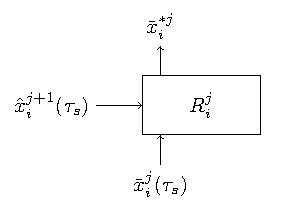
\includegraphics[width=0.5\linewidth,page=1]{automata/rb_correct}
	\caption{Статическая схема корректности для момента времени $\tau_s$.}
	\label{fig:rb_correct_stat0}
\end{figure}

Пусть множество $\mathcal A^0$ состоит из алгоритмов, переводящих пары $(\hat{x},\bar{x})$ в векторы $\bar{\beta}$, составленные из элементов $0,1,\Delta:A(\hat{x},\bar{x})=\bar{\beta}$. Если $\beta_i\in\{0,1\}$, то $\beta_i$ "--- значение величины $\alpha_i$, вычисленное алгоритмом $A$. Если $\beta_i=\Delta$, то алгоритм $A$ не вычислил значение $\alpha_i$ информационного вектора $\bar\alpha$.
	
\begin{Def}
	Алгоритм $A^0$ называется корректным для задачи $Q^0$, если выполнено равенство
	\begin{equation}
		A^0(\hat{x},\bar{x})=\bar{\alpha}.
	\end{equation}
	Алгоритм $A$, не являющийся корректным для $Q^0$, называется некорректным.
\end{Def}

Далее будем считать, что множество $\mathcal A^0$ является совокупностью, вообще говоря, некорректных алгоритмов.
	
\begin{Pred}[аналог теоремы Ю.\,И.~Журавлёва о введении пространства оценок из \cite{Zhuravlev1977}]
	\label{pred:decompositon}
	Каждый алгоритм $A^0\in\mathcal A^0$ представим как последовательность выполнения алгоритмов $R^0$ и $C^0$, где $R^0(\hat{x},\bar{x})=\bar{x}^*$, $\bar{x}^*$ "--- вектор действительных чисел, $C^0(\bar{x}^*)=\bar{\beta}$, $\beta_i\in\{0,1,\Delta\}$.
\end{Pred}
	
\begin{Proof}
	Пусть $D$ "--- алгоритм перехода вектора $\bar{\beta}$ к числовому вектору $\bar{y}$. В качестве $D$ можно рассмотреть, например, $y_i=\beta_i$, если $\beta_i\in\{0,1\}$, и $y_i=1/2$, если $\beta_i=\Delta$. Очевидно, что существует обратный алгоритм $D^{-1}$ перехода от $\bar{y}$ к $\bar{\beta}$. Положим $R^0=A^0\cdot D$, $C^0=D^{-1}$. Тогда очевидно, что $A^0=R^0\cdot C^0=(A^0\cdot D)\cdot D^{-1}=A^0$.
\end{Proof}

Из утверждения \ref{pred:decompositon} следует, что множество алгоритмов $\mathcal A^0$ порождает множества $\mathcal R^0$ и $\mathcal C^0$, которые будем называть \textit{множеством операторов распознавания} и \textit{множеством решающих правил}, соответственно. В качестве операторов из множества $\mathcal R^0$ будем рассматривать операторы $R^0(\hat x,\mathcal Z,\bar x)$.
	
\begin{Def}
	Решающее правило $C^{0*}$ называется корректным на множестве входных векторов $X$, если для всякого вектора $\bar x$ из $X$ существует хотя бы один числовой вектор $\bar x^*$ такой, что $C^{0*}(\bar x^*)=\bar\alpha$, где $\bar\alpha$ "--- информационный вектор входного вектора $\bar x$.
\end{Def}

В множестве операторов $\mathcal R^0$ введём операции умножения на скаляр, сложения и умножения. Пусть $r'$ "--- скаляр, $R',R''\in\mathcal R^0$. Определим операторы $r'\cdot R'$, $R'+R''$ и $R\cdot R''$ следующим образом:
	
\begin{equation}
\label{eq:oper_scalar}
	r'{\cdot}R'=(r'{\cdot}{x_1^*}',\dots,r'{\cdot}{x_l^*}'),
\end{equation}

\begin{equation}
\label{eq:oper_sum}
	R'+R''=({x_1^*}'+{x_1^*}'',\dots,{x_1^*}'+{x_l^*}''),
\end{equation}

\begin{equation}
\label{eq:oper_mult}
	R'{\cdot}R''=({x_1^*}'{\cdot}{x_1^*}'',\dots,{x_1^*}'{\cdot}{x_l^*}'').
\end{equation}
	
\begin{Pred}
	Замыкание $L(\mathcal R^0)$ множества $\mathcal R^0$ относительно операций \eqref{eq:oper_scalar} и \eqref{eq:oper_sum} является векторным пространством.
\end{Pred}

\begin{Def}
	Множество $L(\mathcal A^0)$ алгоритмов $A^0=R^0\cdot C^{0*}$ таких, что $R^0\in L(\mathcal R^0)$, называются линейным замыканием множества $\mathcal A^0$.
\end{Def}

Зафиксируем пару $(\hat{x},\bar{x})$ вектора ожидания и входного вектора. Аналогично \cite{Zhuravlev1977} будем рассматривать задачи $Q^0(\hat{x},\bar{x})$, обладающие следующим свойством относительно множества операторов распознавания $\mathcal R^0$.
	
\begin{Def}
	Если множество векторов $\{R^0(\hat{x},\bar{x})|R^0\in\mathcal R^0\}$ содержит базис в пространстве числовых векторов длины $l$, то задача $Q^0(\hat x,\bar x,\bar\alpha)$ называется полной относительно $\mathcal R^0$.
\end{Def}

\begin{Pred}[аналог теоремы Ю.\,И.~Журавлёва о корректности линейного замыкания из \cite{Zhuravlev1977}]
	\label{pred:correctness}
	Если множество задач $\mathcal Q^0$ состоит лишь из задач, полных относительно $\mathcal R^0$, то линейное замыкание $L(\{R^0\cdot C^{0*}|R^0\in\mathcal R^0\})$ ($C^{0*}$ "--- произвольное фиксированное корректное решающее правило) является корректным относительно $\mathcal Q^0$.
\end{Pred}

\begin{Corollary}
	Пусть $\mathcal A^0$ "--- совокупность некорректных алгоритмов, $\mathcal R^0$ "--- соответствующее множество операторов распознавания, $C^{0*}$ "--- фиксированное корректное решающее правило. Тогда $L(\mathcal A^0)=L(\{R^0\cdot C^{0*}|R^0\in\mathcal R^0\})$ является корректным относительно множества задач $\mathcal Q^0$, если $\mathcal Q^0$ состоит из задач, полных относительно $\mathcal R^0$.
\end{Corollary}

Будем рассматривать только такие задачи $Q^0(\hat{x},\bar{x},\bar{\alpha})$, для которых удовлетворяется следующее условие: ${\exists}k$ такое, что $\bar x$ не равен нулевому вектором. Такое условие является естественным, иначе вектор $\bar{x}$, в котором отсутствуют веса больше $0$, не может рассматриваться как достоверный с точки зрения порогового алгоритма $\mathfrak A_{th}$.
	
\begin{Theorem}
	\label{th:correctness}
	Линейное замыкание $L(\mathcal A^0)$ семейства алгоритмов $\mathcal A^0=\{R^0\cdot C^{0*}|R^0\in\mathcal R\}$ с произвольным корректным решающим правилом $C^*$ и операторами распознавания $\mathcal R$, определёнными шагами \ref{alst:init_start}--\ref{alst:init_end} алгоритма $\mathfrak A_{th}$, является корректным на множестве задач $\mathcal Q^0$.
\end{Theorem}

\begin{Proof}
	В силу утверждения \ref{pred:correctness} достаточно доказать, что произвольная задача $Q^0\in\mathcal Q^0$ является полной относительно $\mathcal R^0$. Доказательство полноты $Q^0$ состоит в прямом построении операторов $R_k, k=1,2,\dots,l$ из $L(\mathcal R^0)$, переводящих пару $(\hat{x},\bar{x}), \hat{x}=(\hat{x}_1,\dots,\hat{x}_l), \bar{x}=(x_1,\dots,x_q)$ в числовой вектор
	\begin{equation} \label{crit:fillness}
		\bar{x}_k^*=(x_{k1}^*,\dots,x_{kl}^*),\ x_{kk}^*=1,\ \forall u\neq k\ x_{ku}^*=0.
	\end{equation} 
	
	Пусть мощность множества $Z_k$ признака $f_k$ равна $N$, норма $\|\bar x\|$ равна $M{\leqslant}q$, максимальная компонента вектора $\bar{x}$ равна $x_{max}$. Зафиксируем величину $k$ и коэффициенты $c_1=\min_v\hat x_v, c_2=\frac{M}{1+M}$. Рассмотрим матрицы предсказания из множеств $Z_1,\dots,Z_l$ признаков $f_1^*,\dots,f_l^*$, удовлетворяющие следующим условиям:
	
 \begin{enumerate}
	 	\item в каждой матрице предсказаний $Z_r^k\in Z_k$ в столбце $\bar{z}_1^r=(z_{11}^r,\dots,z_{1q}^r)$ компонента $z_{1v}^r=1$, если $x_v=x_{max}$, и $z_{1v}^r=0$, если $x_v<x_{max}$; \label{cond:ii}
	 	
	 	\item в каждой матрице предсказаний $Z_r^u\in Z_u, u\neq k$ в столбце $\bar{z}_1^r=(z_{11}^r,\dots,z_{1q}^r)$ компонента $z_{1v}^r=0$ при любых $v$. \label{cond:ij}
 \end{enumerate}
 
 Вычислим величину $x_{kk}^*$. Т.~к. $c_1=\min_u\hat x_u$, то условие $\hat x_k\geqslant c_1$ на шаге \ref{alst:select_f} алгоритма $\mathfrak A_{th}$ автоматически выполняется и функция измерения $\hat f_k$ попадает в множество $\hat F^*$. Из условия \ref{cond:ii} следует, что каждая матрица $Z_r^k\in Z_k$ попадает в множество $Z^*$ на шаге \ref{alst:select_z} алгоритма $\mathfrak A_{th}$:
 \begin{equation}
 	\frac{\|\bar{z}_1^r-\bar{x}\|}{\|\bar{z}_1^r\|+\|\bar{x}\|}<\frac{\sum_v|z_{1v}^r-x_v|}{1+M}<\frac{M}{1+M}=c_2,
 \end{equation}
 так как минимум один компонент в $\bar{z}_1^r$ равен $1$ и существует элемент $x_v>1/2$. В этом случае $x_{kk}^*=\gamma{\cdot}N$, где $\gamma$ "--- весовой коэффициент.
 
 Вычислим величины $x_{ku}^*$. Т.~к. $c_1=\min_v\hat x_v$, то условие $\hat x_u\geqslant c_1$ на шаге \ref{alst:select_f} алгоритма $\mathfrak{A}_{th}$ автоматически выполняется и все функции измерения $\hat f_u$ попадают в множество $\hat F^*$. Из условия \ref{cond:ij} следует, что каждая матрица $Z_r^u\in\mathcal Z_u$ не попадает в множество $Z^*$ на шаге \ref{alst:select_z} алгоритма $\mathfrak A_{th}$:
 \begin{equation}
 	\frac{\|\bar{z}_1^r-\bar{x}\|}{\|\bar{z}_1^r\|+\|\bar{x}\|}=\frac{M}{M}=1>\frac{M}{1+M}=c_2.
 \end{equation}
 В этом случае $x_{ku}^*=0$.
 
 Рассмотрим оператор распознавания $\frac{1}{\gamma\cdot N}R_k(\hat x,\mathcal Z,\bar x)$, матрицы предсказания которого $\mathcal Z=\{Z_1,\dots,Z_l\}$ удовлетворяют условиям \ref{cond:ii}--\ref{cond:ij} и который переводит задачу $Q^0$ в вектор $\bar x_k^*$, причём $\bar x_{kk}^*=1$, а $\bar x_{ku}^*=0, u\neq k$. Данный оператор удовлетворяет критериям (\ref{crit:fillness}) на вектор $\bar x_k^*$, а значит, необходимый базис в пространстве выходных векторов построен. Полнота задачи $Q^0$ доказана.
\end{Proof}

\subsubsection{Произвольный момент времени}
Фиксация момента времени не в начале вычислительного цикла, а на~любом другом значении $\tau_s<t<\tau_s+h_i^j$, приводит к~операторам вида $R_i^j(\hat x_i^j(\tau_s), \mathcal Z_i^j, \omega_{i\Delta t}^j)$, $\Delta t=[\tau_s, t]$, которые кратко будем записывать $R^t$. Использование здесь функции входного воздействия $\omega_{i\Delta t}^j$, которую в виду дискретности времени можно представлять в виде последовательности входных векторов, связано с тем, что состояние распознающего автомата к моменту времени $t$ зависит не только от текущего входа $\bar x_i^j(t)$, но и от предыстории поступления входных векторов с момента начала вычислительного цикла $\tau_s$. Для операторов $R^t$ постановка задачи распознавания выглядит аналогичным образом, как и для операторов $R$ начального времени: задача $Q^t(\hat x_i^j(\tau_s), \omega_{i\Delta t}^j, \bar\alpha)\in\mathcal Q^t$ состоит в построении алгоритма $A^{t*}$, переводящего набор $(\hat x_i^j(\tau_s), \omega_{i\Delta t}^j)$ в информационный вектор $\bar\alpha=(\alpha_1,\dots,\alpha_l)$. 

Определения свойств корректности алгоритма и полноты задачи, а также корректного решающего правила $C^{t*}$, идентичны случаю с начальным моментом времени (Рисунок~\ref{fig:rb_correct_statt}). Аналогично, рассматривая только такие задачи $Q^t(\hat x_i^j(\tau_s), \omega_{i\Delta t}^j, \bar\alpha)$, в которых последовательность $\omega_{i\Delta t}^j$ не содержит нулевых векторов, можно сформулировать следующую теорему (будем далее опускать индексы $i,j$).
	
\begin{figure}[h]
	\centering
	\includegraphics[width=0.5\linewidth,page=2]{automata/rb_correct}
	\caption{Статическая схема корректности для момента времени $\tau_s<t\leqslant\tau_s+h_i^j$.}
	\label{fig:rb_correct_statt}
\end{figure}
	
\begin{Theorem}
	\label{th:correctness_t}
	Линейное замыкание $L(\mathcal A^t)$ семейства алгоритмов $\mathcal A^t=\{R^t\cdot C^{t*}|R^t\in\mathcal R^t\}$ с произвольным корректным решающим правилом $C^{t*}$ и операторами распознавания $\mathcal R^t$, определёнными шагами \ref{alst:cycle_start}--\ref{alst:cycle_end} алгоритма $\mathfrak A_{th}$, является корректным на множестве задач $\mathcal Q^t$.
\end{Theorem}

\begin{Proof}
	Пусть для простоты $\tau_s=0$, т.~е. будем рассматривать первый вычислительный цикл распознающего автомата. Как и в случае доказательства теоремы \ref{th:correctness} будем строить для некоторой задачи $Q^t\in \mathcal Q^t$ базис из операторов $R_k^t,\ k=1,2,\dots,l$ из $\mathcal R^t$, переводящих пару $(\hat x(\tau_s), \omega_{\Delta t})$ в числовой вектор
	\begin{equation}\label{crit:fillness_t}
		\bar x_k^*(t)=(x_{k1}^*,\dots,x_{kl}^*),\ x_{kk}^*=1,\ \forall u\neq k\ x_{ku}^*=0.
	\end{equation}
	
	Зафиксируем, как и в случае доказательства теоремы \ref{th:correctness}, константы $c_1$ и $c_2$: $c_1=\min_v\hat x_v$, $c_2=\frac{M}{1+M}$, где $M$ "--- норма последнего вектора $\bar x(t)$ из последовательности $\omega_{\Delta t}$. Зафиксировав индекс $k$, рассмотрим матрицы предсказания из множеств $Z_1,\dots,Z_l$ признаков $f_1^*,\dots,f_l^*$, удовлетворяющие следующим условиям:
	
	\begin{itemize}
		\item в каждой матрице предсказания $Z_r^k\in Z_k$ первые $t$ столбцов равны соответствующим $t$ элементам последовательности $\omega_{\Delta t}$, а в $t+1$-ом столбце $\bar z_{t+1}^r=(z_{(t+1)1}^r,\dots,z_{(t+1)q}^r)$ компонента $z_{(t+1)v}^r=1$, если $x_v=x_{max}$, и $z_{(t+1)v}^r=0$, если $x_v<x_{max}$, где $x_{max}$ "--- максимальная компонента вектора $\bar x(t)$;
		\item в каждой матрице предсказания $Z_r^u\in Z_u$, $u\not = k$ первые $t$ столбцов также равны соответствующим $t$ элементам последовательности $\omega_{\Delta t}$, а $t+1$-ый столбец $\bar z_{t+1}^r$ "--- нулевой.
	\end{itemize}
	
	Вследствие значения константы $c_1$ условие $\hat x_s\geqslant c_1$ на шаге \ref{alst:select_f} алгоритма $\mathfrak A_{th}$ автоматически выполняется при любых $s$ и все функции измерения попадают в множество $\hat F^*$. Т.~к. до момента времени $t$ столбцы всех матриц из множества $\mathcal Z$ равны друг другу и при этом в точности соответствуют текущему входному вектору, то ни одна матрица не отсеивается на шагах \ref{alst:select_z} и \ref{alst:update_z} алгоритма $\mathcal A_{th}$.
	
	В момент времени $t$ состояние распознающего автомата совпадает с состоянием в начальный момент времени и мы, таким образом, получаем аналогичную доказательству теоремы \ref{th:correctness} ситуацию. В виду выбора константы $c_2$ компонента $x_{kk}^*$ выходного вектора $\bar x^*$ в момент времени $t$ равняется $\gamma\cdot N$, где $\gamma$ "--- весовой коэффициент, а компоненты $x_{uk}^*$, $u\not=k$, равны нулю.
 	
	В итоге, операторы распознавания $\frac{1}{\gamma}R_k^t(\hat x(\tau_s),\mathcal Z_k^t, \omega_{\Delta t})$ ($\gamma$ "--- некоторый весовой коэффициент) выдают выходные вектора, удовлетворяющие условию \ref{crit:fillness_t}, и эти операторы, таким образом, составляют необходимый базис в пространстве выходных векторов. Полнота задачи $Q^t$ доказана.
\end{Proof}

\subsection{Динамические постановки задачи классификации}

\subsubsection{Случай одного распознающего автомата}

Теперь рассмотрим динамическую постановку задачи. Зафиксируем не конкретный момент времени $t$, а полуинтервал времени ${\Delta}t=[\tau_s,\tau_s+h_i^j)$. В~этом случае распознающий автомат $R_i^j$ можно рассматривать как \textit{динамический оператор распознавания} $\hat{R}_i^j(\hat{x}_i^{j+1}(\tau_s), \mathcal{Z}_i^j, \omega_{i\Delta{t}}^j)=\gamma_{i\Delta{t}}^j$, преобразующий  функцию входного воздействия $\omega_i^j$, ограниченную на полуинтервале ${\Delta}t$, в функцию выходной величины $\gamma_i^j$ на том же временном полуинтервале. Так как время полагается дискретным, то действие динамического оператора $\hat{R}_i^j$ можно заменить последовательным по времени действием статических операторов 
\begin{eqnarray}
	R(\hat x_i^{j+1}(\tau_s), \mathcal{Z}_i^j, \bar{x}_i^j(\tau_s)), R^1(\hat x_i^j(\tau_s), \mathcal Z_i^j, \bar x_i^j(\tau_s+1)), \dots,\nonumber\\
	R^{h_i^j-1}(\hat x_i^j(\tau_s), \mathcal Z_i^j, \bar x_i^j(\tau_s+h_i^j-1)),
\end{eqnarray}
выдающих последовательность 
\begin{eqnarray}
	\{\bar{x}_i^{*j}(t)|t\in\Delta t\}=\{\bar{x}_i^{*j}(\tau_s), \bar{x}_i^{*j}(\tau_s+1), \dots, \bar{x}_i^{*j}(\tau_s+h_i^j-1)\}.
\end{eqnarray}
Так как параметр $h_i^j$ фиксирован, то конечные последовательности векторов  $\omega_{i\Delta{t}}^j$ и $\gamma_{i\Delta{t}}^j$ можно считать матрицами размерности $l_i^j\times{h_i^j}$. Далее будем опускать индексы $i$ и $j$.
	
Формулировка задачи в динамическом случае будет выглядеть следующим образом: задача $\hat{Q}(\hat{x}, \omega_{{\Delta}t}, \bar{\alpha})\in\hat{\mathcal Q}$ состоит в построении алгоритма $\hat{\mathcal A}^*$, вычисляющего по поступившему начальному вектору ожиданий $\hat{x}$ и матрице входных воздействий $\omega_{{\Delta}t}$ информационный вектор $\bar{\alpha}$. Однако искомый оператор распознавания $\hat{R}$ должен выдавать матрицу весов присутствия распознаваемых признаков $\gamma_{\Delta{t}}$, столбцы которой должны сходиться (с учётом корректного решающего правила) к информационному вектору: $\lim_{t\to\tau_s+h}\bar{x}^*(t)=\bar{\alpha}$ (Рисунок~\ref{fig:rb_correct_dyn}). 

Т.~к. из всех столбцов выходной матрицы $\gamma_{\Delta t}$ равенство информационному вектору требуется только для последнего столбца, а на остальные накладывается некоторое ограничение, то при разложении алгоритма $\hat A$ будем использовать статический оператор $R^{h-1}$ со следующим ограничением на выходные вектора в моменты времени $0\leqslant t<h$:

\begin{equation}\label{cond:dyn_to_stat}
	\|\bar x^*(\tau_s)-\alpha\|\geqslant \|\bar x^*(\tau_s+1)-\alpha\|\geqslant \dots\geqslant\|\bar x^*(\tau_s+h-1)-\alpha\|,
\end{equation}
где последнее слагаемое приравнивается нулю.  В простейшем случае  $\bar x^*(\tau_s+i)=\bar{\alpha}$, $0\leqslant i < h$. Будем обозначать такие операторы как $\hat R'$, а их множество соответственно $\hat{\mathcal R}'$. 

Определение корректности алгоритма $\hat A$ в данном случае эквивалентно определению в статическом случае.
\begin{figure}[h]
	\centering
	\includegraphics[width=0.5\linewidth,page=3]{automata/rb_correct}
	\caption{Динамическая схема корректности для одиночного распознающего автомата.}
	\label{fig:rb_correct_dyn}
\end{figure}

\begin{Pred}
	\label{st:decompositon_dyn}
	Каждый алгоритм $\hat A\in\hat{\mathcal A}$ представим как последовательность выполнения алгоритмов $\hat R'$ и $C$, где $\hat R'(\hat x, \mathcal{Z}, \omega_{\Delta{t}})=\bar x^*(\tau_s+h-1)$, $\bar x^*(\tau_s+h-1)$ "--- вектор действительных чисел, $C(\bar x^*(\tau_s+h-1))=\bar\beta$, $\bar\beta$ "---вектор значений $\beta_i\in\{0,1,\Delta\}$.
\end{Pred}

В качестве корректного решающего правила $C^*$ используется то же правило, что и в статических случаях. Аналогично статическому случаю вводится определение линейного $L(\hat{\mathcal R}')$ замыкания над множеством $\hat{\mathcal R}'$. 

\begin{Def}
	Если множество векторов $\{\hat R'(\hat x,\omega_{\Delta t})|\hat R'\in\hat{\mathcal R}'\}$ содержит базис в пространстве числовых векторов размерности $l$, то задача $\hat Q(\hat x,\omega_{\Delta t},\bar{\alpha})$ называется полной относительно $\hat{\mathcal R}$.
\end{Def}

\begin{Pred}[аналог теоремы Журавлёва о корректности линейного замыкания из \cite{Zhuravlev1977}]
	\label{pred:correctness_d}
	Если множество задач $\hat{\mathcal Q}$ состоит лишь из задач, полных относительно $\hat{\mathcal R}$, то линейное замыкание $L(\{\hat R'{\cdot}C^*|\hat R'\in\hat{\mathcal R}'\})$ ($C^*$ "--- произвольное фиксированное корректное решающее правило) является корректным относительно $\hat{\mathcal Q}$.
\end{Pred}

Зафиксируем начальный вектор ожиданий $\hat{x}$ и последовательность входных векторов $\omega_{\Delta{t}}$. Если, как и в статическом случае, мы будем рассматривать только такие задачи $\hat{Q}(\hat{x},\omega_{\Delta{t}},\bar{\alpha})$, для которых в матрице $\omega_{\Delta{t}}$ нет нулевых столбцов, то можно сформулировать следующую теорему.

\begin{Theorem}\label{th:correctness_d}
	Линейное замыкание $L(\hat{\mathcal A})$ семейства алгоритмов $\hat{\mathcal A}=\{\hat R'{\cdot}C^*|\hat R'\in\hat{\mathcal R}'\}$ с константным корректным решающим правилом $C^*$ и операторами распознавания $\hat{\mathcal R}'$, определёнными алгоритмом $\mathfrak{A}_{th}$, является корректным на~множестве задач $\hat{\mathcal Q}$.
\end{Theorem}

\begin{Proof}
	В силу того, что динамический оператор $\hat{R}$ эквивалентен по действию введённому статическому оператору $\hat R'$, то для доказательства корректности линейного замыкания необходимо показать полноту произвольной задачи $\hat Q\in\hat{\mathcal Q}$ относительно $\hat{\mathcal R}'$. Для этого, как и ранее, построим такие операторы $\hat R'_k$, $k=1,2,\dots,l$, что 
	
	\[
	\bar x_k^*(\tau_s+h-1)=(x_{k1}^*,\dots,x_{kl}^*), x_{kk}^*=1, \forall u\not=k x_{ku}^*=0.
	\]	
		
	Рассмотрим статические операторы распознавания $R_k^{h-1}$, матрицы предсказания которых строятся по следующим принципам (считаем для упрощения выкладок, что $\tau_s=0$):
	
	\begin{itemize}
		\item в каждой матрице предсказания $Z_r^k\in Z_k$ первые $h-1$ столбцов равны соответствующим $h-1$ столбцам матрицы $\omega_{\Delta t}$, а в $h$-ом столбце $\bar z_{h}^r=(z_{h1}^r,\dots,z_{(hq}^r)$ компонента $z_{hv}^r=1$, если $x_v=x_{max}$, и $z_{hv}^r=0$, если $x_v<x_{max}$, где $x_{max}$ "--- максимальная компонента вектора $\bar x(h-1)$;
		\item в каждой матрице предсказания $Z_r^u\in Z_u$, $u\not = k$ первые $h-1$ столбцов также равны соответствующим $h-1$ столбцам матрицы $\omega_{\Delta t}$, а $h$-ый столбец $\bar z_h^r$ "--- нулевой.
	\end{itemize}
	
	Такие операторы, в силу доказательства теоремы \ref{th:correctness_t}, образуют необходимый базис. Композитный оператор, который строится на их основе, удовлетворяет также и условию \ref{cond:dyn_to_stat} , т.~к. все выходные вектора до момента времени $h-1$ являются единичными векторами $\bar e$, а в момент $h-1$ становятся равными информационному вектору:
	
	\[
		\|\bar e - \alpha\| = \|\bar e - \alpha\| = \dots \leqslant \|\\bar\alpha - \bar\alpha\|.
	\]
	
	Полнота задачи $\hat Q$ доказана.
\end{Proof}
	
\subsubsection{Случай двухуровневой иерархии распознающих автоматов}

Рассмотрим иерархическую постановку задачи, в которой будет учитываться иерархическая связь между операторами распознавания. Будем рассматривать не единичный распознающий автомат, а двухуровневую иерархию $E_j^2$, на каждом уровне которой будет по одному распознающему автомату $R_{i_1}^{j+1}$ и $R_{i_2}^j$. Зафиксируем, как и в~динамическом случае, полуинтервал времени $\Delta t=[\tau_s,\tau_s+h_{i_2}^j)$. Иерархию $E_j^2$ можно рассматривать как \textit{иерархический оператор распознавания} $\hat R_{e,j}^2(\hat x_{i_1}^{j+1}(\tau_s),\mathcal Z_{i_1}^{j+1},\mathcal Z_{i_2}^j,\omega_{i_2\Delta t}^j)=\bar x_{i_1}^{*j+1}$, принимающий функцию входного воздействия $\omega_{i_2\Delta t}^j$ нижнего уровня, ограниченную на полуинтервал времени $\Delta t$, и выдающий вектор весов распознаваемых признаков $\bar x_{i_1}^{*j+1}$. 

Т.~к. в иерархии $E_j^2$ управляющий выходной вектор $R$-автомата $R_{i_1}^{j+1}$ является одновременно и вектором ожидания для $R$-автомата $R_{i_2}^j$, а конечный выходной вектор $\bar x_{i_2}^{*j}$ "--- входным вектором $\bar x_{i_1}^{j+1}$, то действие иерархического оператора $\hat R_{e,j}^2$ можно заменить последовательным действием динамического оператора $\hat R_{i_2}^j(\hat x _{i_2}^{j+1}(\tau_s),\mathcal Z_{i_2}^j,\omega_{i_2\Delta t}^j)$ нижнего уровня и статического оператора $R_{i_1}^{j+1,t}(\hat x _{i_1}^{j+2}(\tau_s),\mathcal Z_{i_1}^{j+1},\bar x_{i_1}^{j+1}(\tau_s))$ верхнего уровня, где для распознающего автомата $R_{i_1}^{j+1}$ рассматривается начальный момент времени вычислительного цикла, соответствующему моменту окончания вычислительного цикла распознающего автомата $R_{i_2}^j$.

Формулировка задачи в~иерархическом случае будет выглядеть следующим образом: задача $\hat Q_{e,j}^2(\hat x_{i_1}^{j+2},\omega_{i_2\Delta t}^j,\bar\alpha_{i_1}^{j+1})\in\hat{\mathcal Q}_{e,j}^2$ состоит в построении алгоритма $\hat A_e$, вычисляющего по поступившему начальному вектору ожиданий $\hat x_{i_1}^{j+2}$ и матрице входных воздействий $\omega_{i_2\Delta t}^j$ значения информационного вектора $\bar\alpha_{i_1}^{j+1}$ (Рисунок~\ref{fig:rb_correct_hier}). Определения свойств корректности алгоритма и полноты задачи, а также корректного решающего правила, в данном случае с~точностью до обозначений совпадают с аналогичными определениями для статического случая.

\begin{figure}[h]
	\centering
	\includegraphics[width=0.5\linewidth,page=4]{automata/rb_correct}
	\caption{Динамическая схема корректности для случая двухуровневой иерархии.}
	\label{fig:rb_correct_hier}
\end{figure}

Зафиксируем начальный вектор ожиданий $\hat x_{i_1}^{j+2}$ и последовательность входных векторов $\omega_{i_2\Delta{t}}^j$. Если мы будем рассматривать только такие задачи $\hat Q_{e,j}^2(\hat x_{i_1}^{j+2},\omega_{i_2\Delta{t}}^j,\bar\alpha_{i_1}^{j+1})$, для которых в матрице $\omega_{i_2\Delta{t}}^j$ нет нулевых столбцов, то можно сформулировать следующую теорему.
		
\begin{Theorem}
	Линейное замыкание $L(\hat{\mathcal A_e})$ семейства алгоритмов $\hat{\mathcal A}_e=\{\hat R_{e,j}^2\cdot\hat C_e^*|\hat R_{e,j}^2\in\hat{\mathcal R}_{e,j}^2\}$ с произвольным корректным решающим правилом $\hat C_e^*$ и операторами распознавания $\hat{\mathcal R}_{e,j}^2$, определёнными алгоритмом $\mathfrak A_{th}$, является корректным на~множестве задач $\hat{\mathcal Q}_{e,j}^2$.
\end{Theorem}

\begin{Proof}
	Доказательство корректности в данном случае сводится к формулировке задачи нижнего уровня $\hat Q_2(\hat x_{i_2}^{j+1},\omega_{i_2\Delta t}^j,\bar\alpha_{i_2}^j)$. Т.~е. необходимо сформировать по~задаче $\hat Q_{e,j}^2$ информационный вектор $\bar\alpha_{i_2}^j$ и вектор ожидания $\hat x_{i_2}^{j+1}$.
	
	Следуя определению вычислительного цикла в алгоритме $\mathfrak A_{th}$, будем считать, что $\hat x_{i_2}^{j+1}$ равен тому управляющему воздействию распознающего автомата $R_{i_1}^{j+1}$, которое было вычислено в начальный момент времени $\tau_s$, т.~е. вектору $\hat x_{i_1}^{j+1}=W(\sum_{\hat f_k\in\hat F^*}\hat x_{ik}^{j+1}\sum_{Z_r^k\in Z^*}\bar z_2^r)$ (см. шаг \ref{alst:init_control} алгоритма $\mathfrak A_{th}$). Каждый компонент $\alpha_{i_2u}^j$ информационного вектора $\bar\alpha_{i_2}^j$ будем вычислять по следующему правилу:
	\begin{equation}
		\alpha_{i_2u}^j=\begin{cases}
			1, & \text{если $\sum\limits_{v=1}^{l_{i_1}^{j+1}}\frac{\alpha_{i_1v}^{j+1}}{|\mathcal{Z}_v|}\sum\limits_{w=1}^{|\mathcal{Z}_v|}z_{1v}^w>0$,}\\
			
			0, & \text{иначе.}
		\end{cases}
	\end{equation}
	Т.~к. входной вектор распознающего автомата $R_{i_1}^j$ равен вектору $\bar\alpha_{i_2}^j$, то такие значения компонентов информационного вектора позволяют удовлетворить ограничениям теоремы \ref{th:correctness_t} (существование ненулевого входного вектора). С другой стороны, формулируя задачу $\hat Q_2(\hat x_{i_2}^{j+1},\omega_{i_2\Delta t}^j,\bar\alpha_{i_2}^j)$ мы попадаем в условия теоремы \ref{th:correctness_d}. В силу этих теорем, можно сделать вывод, что среди алгоритмов линейного замыкания $L(\hat{\mathcal A_e})$ имеется оператор, переводящий пару $(\hat x_{i_1}^{j+1},\omega_{i_2\Delta t}^j)$ в информационный вектор $\bar\alpha_{i_1}^{j+1}$.
\end{Proof}

\subsection{Выводы параграфа \ref{sect3_2}}
На основании исследуемых в работе свойств автоматной функции распознающих автоматов, построенных в соответствии с данными нейрофизиологов для образной компоненты знака, можно сделать следующие выводы:
\begin{enumerate}
\item 
	динамические характеристики образной компоненты описываются в терминах классической теории автоматов;
\item
	построенные автоматы могут быть представлены в виде операторов распознавания, которые можно изучать в рамках классических алгебраических теорий;
\item
	построенные операторы распознавания обладают свойством корректности относительно входных данных и требуемых результатов классификации, что означает существования такого процесса обучения, в рамках которого будут сформирована иерархия базовых элементов, корректно распознающая (классифицирующая) поступающие сигналы.
\end{enumerate}

\clearpage
%% Параграф 3.2
\section{Алгоритм формирования пары <<образ "--- значение>> нового знака} \label{sect3_3}

\subsection{Общая схема образования знака}

В соответствии с тем, что было сказано при описании синтаксического уровня модели картины мира в главе \ref{chapt2}, до того, как происходит связывание компонент знака в единую структуру под одним именем, существуют лишь <<парные>> переходы между компонентами знания агента о том или ином явлении. До моментам именования эти компоненты образуют <<протознак>>:
\begin{itemize}
	\item перцепт становится образом знака после выполнения процедуры именования,
	\item функциональное значение "--- значением знака,
	\item биологический смысл "--- личностным смыслом знака.
	\end{itemize}
	
С введением этой структуры схема алгоритма формирования нового знака будет иметь следующий вид \cite{PanovA2014a}.

\begin{enumerate}
	\label{new_sign_alg}
	\renewcommand\labelenumi{\theenumi .}
	\item\label{stage1} Формирование перцепта.
	\item\label{stage2} Порождение на основе прошлого опыта или на основе прецедентов "--- множества пар вида <<перцепт "--- функциональное значение>> "--- функционального значения объекта.
	\item\label{stage3} Получение субъектом из культурной среды, аккумулированной в системе естественного языка, пары <<имя знака "--- значение>> и оценка специальным механизмом степени близости функционального значения, построенного на стадии \ref{stage1} к значению, полученному из культурной среды; в случае недостаточной близости "--- переход к стадии \ref{stage1} и продолжение формирования перцепта.
	\item\label{stage4} Связывание имени из пары <<имя знака "--- значение>> с перцептом, построенным после завершения выполнения стадий \ref{stage1}--\ref{stage3}; с этого момента перцепт превращается в образ.
	\item Формирование личностных смыслов знака на основе прецедентов действий с предметом.
	\item Связывание имени из пары <<имя знака "--- значение>> со сформированным личностным смыслом. С этого момента функциональное значение превращается в значение, а биологический смысл "--- в личностный смысл.
	\item Продолжение отображения <<биологический смысл "--- перцепт>> включением в область определения отображения личностного смысла, полученного в предыдущем пункте, а в область значений отображения "--- образа из стадии \ref{stage4}.
\end{enumerate}

Наиболее существенным моментом в приведённом алгоритме является итерационный процесс на стадиях \ref{stage1}--\ref{stage3}. Данный параграф будет посвящён исследованию этого процесса.

\subsection{Процедурные и объектные признаки}

Введём семейство бинарных отношений $\{\sqsubset,\sqsubset^1,\sqsubset^2,\dots\}$, определённых на декартовом произведении $\mathcal F\times \mathcal F$. Будем считать, что признак $f_1$ поглощается признаком $f_2$, $(f_1,f_2 )\in\sqsubset$ или $f_1\sqsubset f_2$, в том случае, если $f_1\dashv R_1^j, f_2\dashv R_2^{j+1}$, $R_2^{j+1}$ "--- родительский $R$-автомат по отношению к $R_1^j$ и в множестве матриц предсказания $\mathcal Z_2$ признака $f_2$ существует как минимум одна матрица $Z_r^2$, содержащая некоторый столбец $\bar z_u^r$ с элементом $z_{uv}^r\not=0$, где $v$ "--- индекс признака $f_1$ во входном векторе для распознающего автомата $R_2^{j+1}$ (Рисунок~\ref{fig:rb_measure}).

\begin{figure}[h]
	\centering
	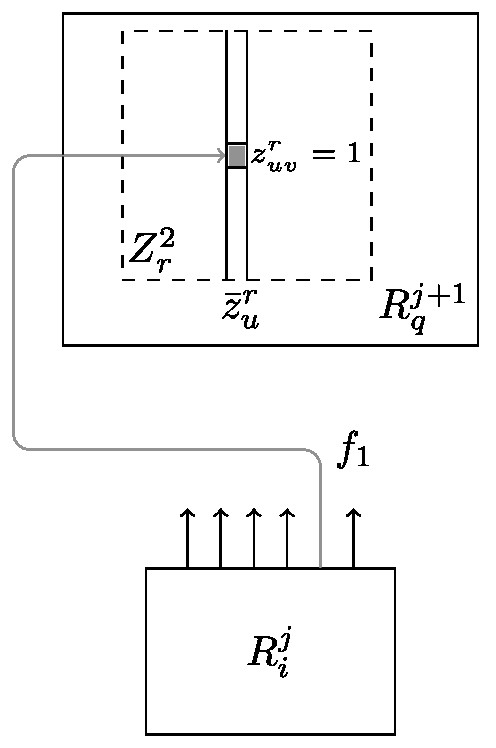
\includegraphics[width=0.3\linewidth]{automata/meas}
	\caption{Определение отношения поглощения на множестве признаков.}
	\label{fig:rb_measure}
\end{figure}

Пара признаков $(f_1,f_2)\in\sqsubset^t$ или $f_1\sqsubset^t f_2$, где $t\in\{1,2,\dots\}$, в~том случае, если $f_1\dashv R_1^j, f_2\dashv R_2^{j+1}$, $R_2^{j+1}$ "--- родительский $R$-автомат по отношению к $R_1^j$ и в множестве матриц предсказания $\mathcal Z_2$ признака $f_2$ существует как минимум одна матрица $Z_r^2$, содержащая $t$–ый столбец $\bar z_t^r$ с~элементом $z_{tv}^r\not=0$, где $v$ "--- индекс признака $f_1$ во~входном векторе для распознающего автомата $R_2^{j+1}$.

Каждый элемент векторов"--~столбцов соотносится с признаком из входного множества признаков распознающего автомата, что означает задание индекса для каждого входного признака. Индекс признака $f_k\in F_i^j$ равен $q$, если ему соответствует $q$-ый элемент векторов"--~столбцов матриц предсказания распознающего автомата $R_i^j$. 

Введём операцию $\Lambda$, которая по множеству матриц распознавания $\mathcal Z_k$ признака $f_k$ определяет два набора индексов столбцов матриц из $Z_k$. Первый набор $I_c=\{i_1^c,i_2^c,\dots\}$, $\forall k\ 0\leqslant i_k^c < h$, составляют индексы \textit{столбцов условий}, в которых ненулевые элементы определяют условия проявления признака $f_k$. Второй набор $I_e=\{i_1^e,i_2^e,\dots\}$, $\forall k\ 0\leqslant i_k^e < h$, состоит из индексов  \textit{столбцов эффектов}, в которых ненулевые элементы определяют эффекты проявления признака $f_k$. Примером реализации процедуры $\Lambda$ может служить алгоритм Норриса по поиску максимального прямоугольного подмножества в бинарном отношении \cite{Norris1977}.

\begin{Def}
	Признаки, для матриц предсказания которых процедура $\Lambda$ выдаёт не пустые множества индексов $I_c$ и $I_e$, будем называть процедурными признаками, остальные "--- объектными признаками.
\end{Def}

Введение данного определения означает, что всё множество признаков делится на два подмножества: $\mathcal F=\mathcal F^{proc}\cup\mathcal F^{obj}$ и $\mathcal F^{proc}\cap\mathcal F^{obj}=\varnothing$.

Для любого процедурного признака выполняются следующие естественные условия:
\begin{itemize}
	\item условие всегда предшествует эффекту,
	\item условие всегда влечёт за собой эффект и
	\item все условия всегда отделены от своих эффектов.
\end{itemize}

Иными словами, если $f_1$ "--- процедурный признак, то если столбец $\bar z_u^r$ матрицы предсказания $Z_r^1$ является столбцом условий, т.~е. $u\in{I_c}$, этот столбец не может одновременно являться столбцом эффектов, т.~е. $u\not\in I_e$, и существует такое $t>0$, что столбец $\bar z_{u+t}^r$ является столбцом эффектов, т.~е. $u+t\in I_e$.

Пополним семейство отношений $\{\sqsubset,\sqsubset^1,\sqsubset^2,\dots\}$ двумя отношениями: $\sqsubset^c$ и $\sqsubset^e$, принадлежность к~которым пары признаков $(f_1,f_2)$ свидетельствует о~том, что признак $f_1$ присутствует соответственно в~столбце условий и эффектов как минимум в~одной матрице предсказания процедурного признака $f_2$.

\subsection{Определение компонент знака}

При образовании нового знака $s$ до того, как формируемая тройка компонент, называемая протознаком, получит имя, будем считать,~что будущему знаку $s$ \textit{соответствует} некоторый признак $f\in\mathcal F$, обладающий перцептом, функциональным значением и биологическим смыслом, которые после завершения процесса формирования знака становятся, соответственно, образом, значением и личностным смыслом.
\begin{Def}
	Если $f_1$ "--- признак, соответствующий знаку $s_1$, то подмножество $\tilde p(f_1)\subseteq\mathcal F$ таких признаков, что $\forall f_i\in\tilde p(f_1) f_i\sqsubset f_1$, будем называть перцептом признака $f_1$ (образом знака $s_1$).
\end{Def}

На множестве всех перцептов $\tilde P$ введём величину $\rho_p(\tilde p(f_1),\tilde p(f_2))$, вычисляемую по~следующему правилу:
\begin{itemize}
	\item если $f_1$ и $f_2$ распознаются разными распознающими автоматами, т.~е. $f_1\dashv R_1^j, f_2\dashv R_2^i$, то $\rho_p(\tilde p(f_1),\tilde p(f_2))=\infty$,
	\item если $f_1$ и $f_2$ распознаются одним и тем~же распознающим автоматами $R_1^j$ со~множеством входных признаков $F_1^j$ мощности $q$ и характерным временем $h$, то
	\begin{equation}
		\rho_p(\tilde p(f_1),\tilde p(f_2))=\min\limits_{\substack{Z_r^1\in Z_1\\Z_s^2\in Z_2}}\frac{1}{q\cdot h}\sum\limits_{u=1}^h\|\bar z_u^r-\bar z_u^s\|.
	\end{equation} 
\end{itemize}

\begin{Pred}
	Величина $\rho_p$ является метрикой на множестве перцептов $\tilde P$.
\end{Pred}

\begin{Proof}
	Свойства тождества и симметрии очевидны вследствие свойств введённой нормы. Проверим неравенство треугольника. В том случае, когда признаки,~распознаются разными автоматами "--- неравенство следует из свойств бесконечности. Во втором случае, в следствие того, что $q$ и $h$ являются константами, то неравенство следует из неравенства треугольника для введённой нормы.
\end{Proof}

\begin{Def}
	Если $f_1$ "--- признак, соответствующий знаку $s_1$, $f_2$ "--- процедурный признак, $f_1\sqsubset^c f_2$, то будем называть $f_2$ элементом функционального значения признака $f_1$ (элементом значения знака $s_1$). Множество всех элементов функционального значения признака $f_1$ будем обозначать $\tilde m(f_1)$.
\end{Def}

На множестве всех функциональных значений $\tilde M$ введём величину $\rho_m(\tilde m(f_1),\tilde m(f_2))$, вычисляемую по следующему правилу:
\begin{equation}\label{eq:m_metr}
	\rho_m(\tilde m_1(f_1),\tilde m_2(f_2 ))=\min\limits_{\substack{f_i\in\tilde m(f_1 )\\f_j\in\tilde m(f_2 )}}\rho_p(\tilde p(f_i ),\tilde p(f_j )).
\end{equation}

\begin{Pred}
	Величина $\rho_m$ является метрикой на множестве функциональных значений $\tilde M$.
\end{Pred}

\begin{Proof}
	Очевидно вследствие того, что функция $\rho_p$ является метрикой, а функция минимума не меняет свойств метрики.
\end{Proof}

\subsection{Семантический уровень обобщения} 

На основе описанной модели компонент знака становится возможным описать процедуры обобщения (см. первую часть работы) на модельном, семантическом уровне. Для этого будем считать, что матрицы предсказания распознающих автоматов были сформированы в процессе обучения (например, с использованием алгоритма HTM \cite{Hawkins2009} или THSOM \cite{Koutn2008}). При рассмотрении множества матриц предсказания $\mathcal Z$ некоторого распознающего автомата возникают следующие три основных случая:

\begin{itemize}
	\item \textit{Внутреннее обобщение}. Будем называть схожими, такие матрицы из подмножества $Z'_k=\{Z_1^k,Z_2^k\dots,Z_m^k\}$ множества матриц предсказания $Z_k$ некоторого признака $f_k$, для которых при $\forall i,j,l$ таких, что $Z_i,Z_j\in Z'_k,l\in\{0,\dots,h\}$ выполняется $card(z_l^i\wedge z_l^j)<c_3$, где $c_3$ "--- некоторая константа. Обобщение в этом случае заключается в замене подмножества схожих матриц $Z'_k$ одной обобщённой $Z^*=(\bigwedge\limits_{Z_q\in Z'_k}\bar z_1^q,\bigwedge\limits_{Z_q\in Z'_k}\bar z_2^q,\dots,\bigwedge\limits_{Z_q\in Z'_k}\bar z_h^q)$. Таким образом, осуществляется кластеризация множества матриц предсказания признака $f_k$, контролируемая одним параметром близости $c_3$.
	\item \textit{Конкретизация}. В~тех случаях, когда получаемые с использованием описанной выше меры близости кластеры матриц предсказания признака $f_k$ расходятся достаточно сильно, образуются новые конкретизированные признаки для каждого кластера и соответственно расширяется множество выходных признаков $F^*$ распознающего автомата.
	\item \textit{Внешнее обобщение}. В~том случае когда во~всех матрицах предсказания $R$-автоматов, являющихся родительскими по отношению к распознающему автомату $R$, $i$-ые и $j$-ые компоненты всех столбцов матриц принимают одинаковые значения, выходные признаки $f_i,f_j\in F^*$, соответствующие этим компонентам, обобщаются в один признак с объединённым множеством матриц предсказания. При этом возможно и дальнейшее внутреннее обобщение.
\end{itemize}

Отдельно необходимо рассмотреть случай \textit{абстрагирования}, когда несколько выходных признаков одного или нескольких распознающих автоматов в результате работы процедуры обобщения на синтаксическом уровне (см. первую часть работы) формируют новый признак $f^*$ в некотором $R$-автомате $R^*$, лежащем на следующем уровне иерархии. В этом случае матрица предсказания будет состоять из единственного столбца с ненулевыми элементами, которые соответствуют признакам, составляющим данную категорию.

И, наконец, ещё один случай обобщения на семантическом уровне заключается в образовании ролевой структуры процедурных признаков. Рассмотрим случай, когда столбцы условий или эффектов некоторых матриц предсказания процедурного признака $f_p$ различаются только в двух компонентах, т.~.е. $i$-ая компонента в некоторых столбцах равна $1$, а в других "--- $0$, а $j$-ая компонента наоборот "--- в первых равна $0$, а во вторых "--- $1$. Если соответствующие этим компонентам признаки в результате абстрагирования попали в некоторую общую категорию $f_{cat}$, то к множеству матриц предсказания признака $f_p$ добавляется матрица с новой компонентой, соответствующей признаку $f_{cat}$ и обнулёнными компонентами $i$ и $j$. Данная процедура легко распространяется на случай, когда количество элементов категории $f_{cat}$ в матрицах предсказания признака $f_p$ больше двух. Таким образом, для процедурного признака $f_p$ появляется обобщённая, ролевая матрица предсказания.

\subsection{Свойства на множестве признаков}

В целях дальнейшего изложения рассмотрим подробнее строение матрицы предсказания процедурного признака. Матрицу предсказания $Z_r^p$ процедурного признака $f_p$ всегда можно представить в следующем виде:
\begin{equation}
Z_r^p=(\bar z_1^{r,c},\dots,\bar z_{j_1}^{r,c},\bar z_{j_{1+1}}^{r,e},\dots,\bar z_{i_1}^{r,e},\dots,\dots,\bar z_{i_{k-1}+1}^{r,c},\dots,\bar z_{j_k}^{r,c},\bar z_{j_k+1}^{r,e},\dots,\bar z_{i_k}^{r,e}),
\end{equation}
где $\bar z_j^{r,c}$ "--- столбцы причин, $\bar z_i^{r,e}$ "--- столбцы следствий. 

Величину $k$ будем называть \textit{сложностью} процедурного признака. В~дальнейшем будем рассматривать простые матрицы предсказаний $k$-сложного процедурного признака:
\begin{equation}
Z_r^p=(\bar z_1^{r,c},\bar z_2^{r,e},\dots,\dots,\bar z_{2\cdot k-1}^{r,c},\bar z_{2\cdot k}^{r,e}).
\end{equation}
Краткая форма $k$-сложного процедурного признака $f_p$ имеет матрицу предсказания, в которой оставлены только первый столбец условий и последний столбец эффектов.

Любой односложный, или элементарный, процедурный признак $f_p$, распознаваемый автоматом $R_i^j$, можно представить в виде правила $r_p=(F_C(f_p),F_A(f_p),F_D(f_p))$, в котором:
\begin{itemize}
	\item $F_C (f_p )\subseteq F_i^j$ "--- множество признаков "--- условий правила: $\forall f\in F_C(f_p)$ $f\sqsubset^c f_p$;
	\item $F_A(f_p)\subseteq F_i^j$ "--- множество добавляемых правилом признаков: $\forall f\in F_A(f_p)$ $f\sqsubset^e f_p,f\not\sqsubset^c f_p$;
	\item $F_D(f_p)\subseteq F_i^j$ "--- множество удаляемых правилом признаков: $\forall f\in F_D(f_p)$ $f\not\sqsubset^e f_p,f\sqsubset^c f_p$.
\end{itemize}

Очевидно, выполняются следующие соотношения: $F_A(f_p)\cap F_D(f_p)=\varnothing, F_A(f_p)\cap F_C(f_p)=\varnothing, F_D(f_p)\subseteq F_C(f_p)$.

\begin{Def}\label{def:feas}
	Процедурный признак $f_p^1\dashv R_i^j$ c матрицей предсказания $Z=(\bar z_1^c,\bar z_2^e)$ выполняется на векторе $\bar z$ длины $q$, где $q$ "--- длина входного вектора $R$-автомата $R_i^j$, если $\bar z\cdot \bar z_1^c=\bar z_1^c$.
\end{Def}

Здесь под операцией <<$\cdot$>> подразумевается покомпонентное умножение битовых векторов. Если в качестве вектора $\bar z$ в определении (\ref{def:feas}) взять столбец условий некоторого признака $f_p^2$, то будем говорить, что процедурный признак $f_p^1$ выполним в~условиях процедурного признака $f_p^2$, если 
\begin{itemize}
	\item оба признака распознаются одним и тем~же распознающим автоматом $R_i^j$ и признак  $f_p^1$ выполняется на~столбце условий матрицы предсказания признака $f_p^2$,
	\item $f_p^1\dashv R_i^{j_1}, f_p^2\dashv R_k^{j_2}$, $i\not=k$, $F_C(f_p^1 )\subseteq F_C(f_p^2)$ и признак  $f_p^1$ выполняется на~столбце условий матрицы предсказания признака $f_p^2$. 
\end{itemize}

\begin{Def}
	Будем говорить, что два процедурных признака $f_p^1$ и $f_p^2$ конфликтуют, если выполнено как минимум одно из~следующих условий:
	\begin{itemize}
		\item $F_D(f_p^1)\cap F_A(f_p^2)\not=\varnothing$,
		\item $F_D(f_p^2)\cap F_A(f_p^1)\not=\varnothing$,
		\item $F_D(f_p^1)\cap F_C(f_p^2)\not=\varnothing$,
		\item $F_D(f_p^2)\cap F_C(f_p^1)\not=\varnothing$.
	\end{itemize}
\end{Def}

\begin{Def}
	Результатом операции приведения вектор"--~столбца $\bar z$ матрицы распознавания $R$-автомата $R_{i_1}^{j_1}$ к $R$-автомату $R_{i_2}^{j_2}$ будем называть такой вектор $\bar z'$ длины $q_{i_2}^{j_2}$, $k$-ый элемент которого $z'_k=1$, если признак $f\in F_{i_1}^{j_1}$ с индексом $k$ равен признаку $f'\in F_{i_2}^{j_2}$ с тем же индексом и $z_k=1$, иначе $z'_k=0$, и обозначать его $(\bar z\rightarrow R_{i_2}^{j_2})=\bar z'$.
\end{Def}

\begin{Def}
	Результатом операции приведения вектор"--~столбца $\bar z$ матрицы распознавания $R$-автомата $R_{i_1}^{j_1}$ к $R$-автомату $R_{i_2}^{j_2}$ по столбцу $\bar z'$ матрицы распознавания из множества  $\mathcal Z_{i_2}^{j_2}$ будем называть такой вектор $\bar z''$ длины $q_{i_2}^{j_2}$, элемент которого $z''_k=1$, если признак $f\in F_{i_1}^{j_1}$ с индексом $k$ равен признаку $f'\in F_{i_2}^{j_2}$ с тем же индексом, $z'_k=1$ и $z_k=1$, иначе $z''_k=0$, и обозначать $(\bar z\xrightarrow{\bar z'} R_{i_2}^{j_2})=\bar z''$.
\end{Def}

\subsection{Опыт наблюдения и алгоритм $\mathfrak A_{pm}$}

Будем считать, что у субъекта имеется опыт наблюдения, который выражается в виде отношения $\Psi_p^m: \Psi_p^m(\tilde p)=\tilde m$, в том случае, если $\tilde p\in\tilde P$ является перцептом некоторого признака $f$, а $\tilde m\in\tilde M$ "--- функциональным значением того же признака $f$.

На странице \pageref{alg:cycle_pm_start} и \pageref{alg:cycle_pm_end} представлен алгоритм доопределения функции $\Psi_p^m$, который и представляет собой суть итерационного процесса во время образования знака согласно алгоритму на странице \pageref{new_sign_alg}. Доопределение проводится на~новую пару $(\tilde p,\tilde m)$, где функциональное значение $\tilde m$ строится в сравнении с эталоном $\tilde m^0$, а перцепт $\tilde p$ формируется на основе множества признаков, входящих в область текущую определения $\hat F=dom\ \Psi_p^m$. Доопределение функции $\Psi_p^m$ означает формирование нового признака $f^*$, т.~е. его первой матрицы предсказания $Z^*$ в~рамках распознающего автомата $R^*$.

\begin{algorithm}[h]
	\caption{Алгоритм $\mathfrak{A}_{pm}$ (часть I)}
	\label{alg:cycle_pm_start}
	\begin{algorithmic}[1]
			\Require $\tilde m^0=\{f_p^0\}, \Psi_p^m, \hat F=dom\ \Psi_p^m\subseteq \mathcal F$;
	\algrule
	\State $Z_p^0 := \{\bar z_1^{c0},\bar z_2^{e0}\}$ "--- матрица предсказания признака $f_p^0$;
	\State $\tilde p^{(0)} := \varnothing$, $\tilde m^{(0)} := \varnothing$;
	\State $R_0\not\in\mathcal R$ "--- фиктивный распознающий блок, для которого $F_0^*=\{f_p^0\}$;
	\State $Z^{(0)} := \varnothing$, $Z_p^{(0)} := \{\bar 0, \bar 0\}$;
	\State $q^{(0)} := 0$, $t := 0$;
	
	\While{$Z_p^{(t)}\not=Z_p$ или $t<|\hat F|$}
		\State $f\in\hat F$ "--- первый не рассмотренный ранее признак; 
		\State $Z=\{\bar z_1,\bar z_2,\dots,\bar z_q\}$ "--- его матрица предсказания;
		\If{$\exists \tilde m=\{f_p\}\in \tilde M$ такое, что $(\tilde p(f),\tilde m)\in\Psi_p^m$, $f_p$ выполним в условиях признака $f_p^0$ и $\nexists f'$ такого, что $f'\in\tilde p^{(t)}$,$\tilde m'=\{f'_p\}\in\tilde M$, $(\tilde p(f'),\tilde m')\in\Psi_p^m$, $f'_p$ конфликтует с $f_p$}\label{alst:find_m}
			\State $\tilde p^{(t+1)}=\tilde p^{(t)}\cup\{f\}$;
			\State $Z_p=\{\bar z_1^{c},\bar z_2^{e}\}$ "--- матрица предсказания признака $f_p$;
	
			\If{$\exists R_i^j$ такой, что $\tilde p^{(t+1)}\subseteq F_i^j$}
				\State $R_i^{j(t+1)}:=R_i^j$;
			\Else
				\State $R_i^{j(t+1)}:=\argmax\limits_{\mathcal R} (F_i^j\cap\tilde p^{(t+1)})$;
				\State $F_i^{j(t+1)}:=F_i^{j(t)}\cup\tilde p^{(t+1)}$;
			\EndIf

		\algstore{algst:store2}
	\end{algorithmic}
\end{algorithm}

\begin{algorithm}[h]
	\caption{Алгоритм $\mathfrak{A}_{pm}$ (часть II)}
	\label{alg:cycle_pm_end}
	\begin{algorithmic}[1]
		\algrestore{algst:store2}
					\State $q^{(t+1)}=\max\{q^{(t)},q\}$;
			\State $Z^{(t+1)}:=\{\bar z_1^{(t+1)},\bar z_2^{(t+1)},\dots \bar z_{q^{(t+1)}}^{(t+1)}\}$, где $\bar z_i^{(t+1)}=\bar z_i^{(t)}\vee \bar z_i$, если $i\leqslant q$ и $i\leqslant q^{(t)}$, $\bar z_i^{(t+1)}=\bar z_i^{(t)}$, если $i>q$ и $\bar z_i^{(t+1)}=\bar z_i$, если $i > q^{(t)}$;
			
			\State $Z_p^{(t+1)}:=\{\bar z_1^{c(t+1)},\bar z_2^{e(t+1)}\}$, где $\bar z_1^{c(t+1)}=\bar z_1^{c(t)}\vee (\bar z_1^c\rightarrow R_0)$, $\bar z_2^{e(t+1)}=\bar z_2^{e(t)}\vee (\bar z_2^e\xrightarrow{\bar z_2^{e0}} R_0)$;
			
			\State $f_p^{(t+1)}$ "--- признак с матрицей предсказания $Z_p^{(t+1)}$;
			
			\State $\tilde m^{(t+1)}=\{f_p^{(t+1)}\}$;
		\EndIf
	
		\State $t=t+1$;
	\EndWhile

	\State $R^*=R_i^{j(t)}$;
	\State $Z^*=Z^{(t)}$;
	\State $\mathcal Z^{*}=\mathcal Z_i^{j(t)}\cup\{Z^*\}$;	
	
	\Return $\Psi_p^m$, доопределённую на паре $(\tilde p, \tilde m)$, где $\tilde p=\tilde p^{(t)}$, $\tilde m=\tilde m^{(t)}$.
	\end{algorithmic}
\end{algorithm}

Для обоснования данного алгоритма необходимо доказать сходимость функциональных значений, которые строятся в процессе его выполнения, к эталонному значению $\tilde m^0$.

%============================================================================================================================

\subsection{Корректность алгоритма $\mathfrak A_{pm}$} \label{sect3_4}

\begin{Theorem}[о корректности алгоритма $\mathfrak A_{pm}$]
	Алгоритм $\mathfrak A_{pm}$ корректен, т.~е. элементы последовательности функциональных значений $\langle\tilde m^{(0)},\tilde m^{(1)},\dots,\tilde m^{(t)}\rangle$, которая строится с помощью алгоритма $\mathfrak A_{pm}$ для функционального значения $\tilde m^0$, приближаются к $\tilde m^0$ в смысле метрики (\ref{eq:m_metr}).
\end{Theorem}

\begin{Proof}
	Рассмотрим два элемента последовательности $\tilde m^{(t)}=\{f_p^{(t)}\}$ и $\tilde m^{(t+1)}=\{f_p^{(t+1)}\}$. Соответствующие матрицы предсказания будут иметь следующий вид:
	\begin{equation}
		Z_p^{(t)}=\{\bar z_1^{c(t)},\bar z_2^{e(t)}\},\ Z_p^{(t+1)}=\{\bar z_1^{c(t+1)},\bar z_2^{e(t+1)}\}.
	\end{equation}
	Если на шаге \ref{alst:find_m} алгоритма $\mathfrak A_{pm}$ на $(t+1)$-й итерации не был найден подходящий признак, то матрицы $Z_p^{(t)}$ и $Z_p^{(t+1)}$ равны. Рассмотрим случай, когда был найден подходящий признак $f'$ с функциональным значением $\tilde m'=\{f'_p\}$ с соответствующей матрицей предсказания $Z'=(\bar z'^c_1,\bar z'^e_2)$.
	
	В том случае, если на шаге \ref{alst:find_m} был найден признак $f'_p$ то матрицы $Z_p^{(t)}$ и $Z_p^{(t+1)}$ будут отличать в своих двух столбцах:
	\begin{equation}
		\bar z_1^{c(t+1)}=\bar z_1^{c(t)}\vee (\bar z'^c_1\rightarrow R_0),\ \bar z_2^{e(t+1)}=\bar z_2^{e(t)}\vee (\bar z'^e_2\xrightarrow{\bar z_2^{e0}} R_0).
	\end{equation}
	По определению расстояние между функциональными значениями $\tilde m^{(t)}$ и $\tilde m^0$ примет следующее значение:
	\begin{eqnarray}
		\rho_m(\tilde m^{(t)},\tilde m^0)=\min\limits_{\substack{f_i\in\tilde m^{(t)}\\f_j\in\tilde m^0}}\rho_p(\tilde p(f_i),\tilde p(f_j ))=\rho_p(\tilde p(f'_p),\tilde p(f_p))=\nonumber \\
		=\frac{1}{q\cdot h}\sum\limits_{\substack{\bar z_u^{1(t)}\in Z_p^{(t)}\\\bar z_u^2\in Z_p^0}}\|\bar z_u^{1(t)}-\bar z_u^2\|.
	\end{eqnarray}
	Аналогично для $\tilde m^{(t+1)}$:
	\begin{equation}
		\rho_m(\tilde m^{(t+1)},\tilde m^0)=\frac{1}{q\cdot h}\sum_{\substack{\bar z_u^{1(t+1)}\in Z_p^{(t+1)}\\\bar z_u^2\in Z_p^0}}\|\bar z_u^{1(t+1)}-\bar z_u^2\|.
	\end{equation}
	Рассмотрим разность 
	\begin{eqnarray}
		\rho_m(\tilde m^{(t)},\tilde m^0)-\rho_m(\tilde m^{(t+1)},\tilde m^0)=\frac{1}{q\cdot h}(\|\bar z_1^{c(t)}-\bar z_1^{c0}\|+\|\bar z_2^{e(t)}-\bar z_2^{e0}\|-\nonumber \\
		-\|\bar z_1^{c(t+1)}-\bar z_1^{c0}\|-\|\bar z_2^{e(t+1)}-\bar z_2^{e0}\|)=\frac{1}{q\cdot h}(\|\bar z_1^{c(t)}-\bar z_1^{c0}\|+\nonumber \\
		+\|\bar z_2^{e(t)}-\bar z_2^{e0}\|-\|\bar z_1^{c(t)}\vee (\bar z'^c_1\rightarrow R_0)-\bar z_1^{c0}\|-\nonumber \\
		-\|\bar z_2^{e(t)}\vee (\bar z'^e_2\xrightarrow{\bar z_2^{e0}} R_0)-\bar z_2^{e0}\|),
	\end{eqnarray}
	где $\bar z_1^{c0}$, $\bar z_2^{e0}$ "--- столбцы матрицы предсказания процедурного признака $f_p^0$, соответствующего функциональному значению $\tilde m^0$.
	
	Так как $f'_p$ выполним на первом столбце матрицы предсказания признака $f_p^0$, то после применении операции приведения $\bar z'^c_1\rightarrow R_0$ в результирующем векторе единицы появляются только на тех же местах что и в векторе $\bar z_1^{c0}$. Это означает, что в векторе $\bar z_1^{c(t)}\vee (\bar z'^c_1\rightarrow R_0)-\bar z_1^{c0}$ по сравнению с вектором $\bar z_1^{c(t)}$  единицы находятся только в тех же местах, что и в векторе $\bar z_1^{c0}$, а новых нулей не появляется. В следствие чего разность $\|\bar z_1^{c(t)}-\bar z_1^{c0}\|-\|\bar z_1^{c(t)}\vee (\bar z'^c_1\rightarrow R_0)-\bar z_1^{c0}\|$ всегда больше либо равна нулю.
	
	Так как для столбцов эффектов применяется операция приведения по столбцу, то единицы в результирующем векторе остаются только на тех местах, на которых одновременно находятся единицы в приводимом векторе и векторе, по которому осуществляется приведение. В связи с этим разность $\|\bar z_2^{e(t)}-\bar z_2^{e0}\|-\|\bar z_2^{e(t)}\vee (\bar z'^e_2\xrightarrow{\bar z_2^{e0}} R_0)-\bar z_2^{e0}\|$ также больше либо равна нулю.
	
	Так как обе разности в скобках выражения для $\rho_m(\tilde m^{(t)},\tilde m^0)-\rho_m(\tilde m^{(t+1)},\tilde m^0)$ больше либо равны нулю, то отсюда следует, что функциональное значение $\tilde m^{(t+1)}$ ближе или по крайней мере находится на том расстоянии от $\tilde m^0$, чем к $\tilde m^{t}$. В виду произвольности выбора итерации $t$, это приводит к тому, что элементы всей последовательности $\langle\tilde m^{(0)},\tilde m^{(1)},\dots\rangle$ приближаются к $\tilde m^0$ в смысле использованной метрики (\ref{eq:m_metr}). 
\end{Proof}


%\newpage
%============================================================================================================================

\clearpage

% Заключение
\conclusion

В~работе были получены следующие основные результаты.

\begin{enumerate}
	\renewcommand\labelenumi{\theenumi.}
	\item Построена модель компонент знака "--- элемента картины мира субъекта деятельности в рамках сегодняшних представлений о функционировании мозга и психики человека.
	\item Построены четыре типа операторов распознавания (два статических оператора, динамический и иерархический операторы) в терминах алгебраической теории для образной компоненты знака.
	\item Доказаны теоремы корректности линейных замыканий множеств построенных в работе операторов распознавания (статических, динамического и иерархического).
	\item Построен алгоритм формирования и связывания двух компонент знака: образа и значения.
	\item Исследована сходимость итерационного алгоритма формирования и связывания двух компонент знака.
\end{enumerate}

\clearpage

% Список литературы
\bibliography{../../biblio/umain}
\bibliographystyle{ugost2008}

% Список иллюстративного материала
\listoffigures

% Приложения
\appendix
\chapter{Типы картин мира} \label{AppendixA}

В соответствие с предыдущим параграфом в результате работы механизмов самоорганизации на множестве знаков формируются три основных типа структур. Каждую из них в соответствии с \cite{Osipov1990} будем называть неоднородной семантической сетью или, поскольку это не приводит к недоразумениям, семантической сетью. Рассмотрим три таких сети.
\begin{enumerate}
	\renewcommand\labelenumi{\theenumi.}
	\item Семантическую сеть $H_P=\langle 2^P,\mathfrak R_P\rangle$ на множестве образов, где $\mathfrak R_P=\{R_1,R_2,R_3,R_4\}$ "--- семейство отношений на образах.
	\item Семантическую сеть $H_A=\langle 2^A,\mathfrak R_A\rangle$ на множестве личностных смыслов, где $\mathfrak A=\{R_5\}$ "--- семейство отношений на личностных смыслах.
	\item Семантическую сеть $H_M=\langle 2^M,\mathfrak R_M\rangle$ на множестве значений знаков, где $\mathfrak R_M=\{R_1^\prime,R_3^\prime,R_6,R_7\}$ "--- семейство отношений на значениях.
\end{enumerate}

Тройку объектов $H=\langle H_P,H_A,H_M\rangle$ будем называть семиотической сетью. Переходы между сетями $H_P$, $H_A$, $H_M$ реализуются, как следует из предыдущего, посредством процедур $\Psi_m^a$, $\Psi_a^p$ и $\Psi_p^m$.

Уровень имён знаков может наследовать каждую из описанных выше семантических сетей. Благодаря такому наследованию можно говорить о формировании той или иной семантической сети на уровне знаков (не только на уровне их компонент).

Предлагается выделять три типа картины мира: рациональную, житейскую и мифологическую \cite{Chudova2012a}. 
Мы видели, что на сети $H_P$ можно определить операции обобщения (и классификации) по признакам (раздел \ref{subsect_2_3_1}). Именно эти операции характерны для рациональной картины мира. На основании этих соображений и ряда психологических экспериментов (описание которых остаётся за пределами настоящего доклада) можно полагать, что именно сеть на множестве образов (и ее наследование на уровень имён знаков) лежит в основе рациональной картины мира. Здесь надо подчеркнуть важность слов <<в основе>>. Все типы картин мира используют сети на образах, на смыслах и сценариях, но есть некоторая <<управляющая>> сеть, которая служит для формулирования цели, поиска подходящих действий, вызова сценариев и изменения личностных смыслов. Например, в рациональной картине мира в сети на образах выполняется выработка цели, затем в сети на значениях находятся подходящие роли в сценарии как условия выполнения действий для достижения цели, далее учитываются смыслы объектов, которые могут быть мотивами или препятствиями, или средствами для достижения цели \cite{Chudova2014}. Отметим, что могут быть описаны и вырожденные картины мира, в которых используются не три, а только две сети (например, только $H_A$ и $H_M$ для нигилистической картины мира \cite{Chudova2012a}). 

Житейская картина мира характеризуется следованием некоторым стереотипам или сценариям поведения. Таким образом, наследование на уровень имён знаков сети на значениях приводит к формированию житейской картины мира. Здесь также следует отметить, что сеть на значениях является лишь ведущей: моделирование, например, картины мира чиновников реализуется на двух сетях "--- сценариев и личностных смыслов. Поэтому при возникновении нового предмета потребности (например, выделение бюджета на науку и культуру) находится сценарий, в котором смысл цели из амбивалентного превращается в смысл препятствия. Поскольку в этом процессе не присутствуют образы, то речь идёт о вырожденной картине мира. В общем случае в житейской картине мира выбранный сценарий (на сети значений) пополняется образами тех объектов (в том числе партнёров), которые наилучшим образом (в соответствии с оценкой на сети смыслов) могут исполнять записанные в сценарии роли (например, начальник подбирает исполнителей в новую группу для <<хорошего>> выполнения нового вида работ или жених и невеста составляют список гостей на свадьбу в соответствии со своими представлениями о том, как должна выглядеть <<хорошая>> свадьба).

В мифологической картине мира каждая роль имеет неизменный смысл и заданный образ, т.е. ведущей в этом случае является сеть на смыслах. Иначе говоря, наследование сети $H_A$ на уровень имён знаков приводит к формированию мифологической картины мира.

\chapter{Модель функции целеполагания на синтаксическом уровне} \label{AppendixB}

Задача управления поведением субъекта деятельности включает в себя фазы планирования и исполнения плана \cite{Osipov2002c,Osipov2003a,Osipov2008b}. Первая задача планирования заключается в выдвижении цели "--- целеполагании. Применим развитый выше аппарат к решению этой задачи. Синтез плана и его исполнение будут рассмотрены во второй части статьи.
Целеполагание "--- сложный процесс, который включает в себя не только выдвижение цели, но и определение условий и конкретного способа ее достижения. Как уже было сказано, характер процесса целеполагания определяется типом картины мира (КМ) субъекта. В случае житейской КМ ведущим компонентом является значение, т.е. субъект отталкивается от сюжетно"--~ролевой структуры и использует уже существующие знаки, чтобы выбрать подходящую ситуацию, которая и будет целевой.
Для обозначения операции переходов на сети значений, образов и личностных смыслов введём недетерминированный оператор переходов $Tr$, действующий на булеанах $2^P$, $2^A$ и $2^M$: $Tr(x)=x^\prime$, где $x,x^\prime\in 2^A$ или $x,x\prime\in 2^P$, или $x,x^\prime\in 2^M$. Левая композиция оператора $\Psi_x^y$, где $x\in\{m, a, p\}$, $y\in\{m, a, p\}$ (т.е. любого из операторов  $\Psi_p^m$, $\Psi_m^a$ или $\Psi_a^p$), с оператором переходов по сети $y$ обозначим как $\underline{\Psi}_x^y:\underline{\Psi}_x^y=\Psi_x^y\circ Tr(x)$, где $Tr(x)=x^\prime$, $x\in 2^A$ или $x\in 2^P$, или $x\in 2^M$ и $x^\prime\in 2^A$, или $x^\prime\in 2^P$, или $x^\prime\in 2^M$. Под композицией операторов будем понимать применение левого оператора к результату применения правого оператора. Правая композиция оператора $\Psi_x^y$ , где $x\in\{m, a, p\}$, $y\in\{m, a, p\}$, с оператором переходов по сети y обозначим как $\overline{\Psi}_x^y: \overline{\Psi}_x^y=Tr(y)\circ\Psi_x^y$, где $Tr(y)=y^\prime$, $y\in 2^A$ или $y\in 2^P$, или $y\in 2^M$ и  $y^\prime\in 2^A$, или $y^\prime\in 2^P$, или $y^\prime\in 2^M$. Например, левая композиция оператора   с оператором перехода по сети образов запишется как $\underline{\Psi}_p^m=\Psi_p^m\circ Tr(y)$.

Процесс целеполагания осуществляется в рамках какой-либо деятельности. Будем рассматривать случай, когда мотив деятельности осознан, т.е. знак предмета потребности включён в картину мира субъекта деятельности. Тогда мотивом деятельности (в житейской картине мира) является значение ($m$) этого знака. Мотив удовлетворяется, когда существует знак, такой, что результатом применения правой композиции оператора   с оператором переходов ($Tr(p)\circ\Psi_a^p$) к личностному смыслу этого знака является образ знака предмета потребности. (Или на семантическом уровне: существует знак, такой, что результатом некоторого действия, интерпретирующего личностный смысл этого знака, выступает образ знака предмета потребности.)

Тогда знак, результатом применения к которому правой композиции оператора $\Psi_a^p$ с оператором переходов является образ знака предмета потребности, будем называть целевым знаком. Или на семантическом уровне: целевым будем называть такой знак, в структуре личностного смысла которого существует действие, применение которого приводит к формированию признаков образа предмета потребности (удовлетворению потребности). Процесс целеполагания, таким образом, заключается в построении такой последовательности знаков, которая заканчивается знаком, из которого достижим мотив, т.е. удовлетворяется потребность.

В соответствии с разд. 3.4 значение знака будем представлять в виде множества пар <<действие "--- роль предмета в этом действии>>, образ ($p$) такого знака "--- в виде набора свойств, т.~е. пар <<признак "--- значение признака>>, личностный смысл ($a$) "--- в виде правила, соответствующего действию субъекта с предметом; условие и эффект действия такого правила задаются в виде множества свойств.

Далее, $s^*$ "--- знак, экземпляр значения которого $\mu^*$ является мотивом деятельности. В приведённом ниже алгоритме целеполагания будем использовать как синтаксические, так и семантические соображения, особенно не подчёркивая этого обстоятельства.

\textbf{Алгоритм GS.}

\textbf{Вход}: знак предмета потребности $s^*$, мотив $\mu^*$.

\textbf{Шаг 1}: переход $\mu^*\rightarrow a_1$ (применяется оператор $\underline{\Psi}_m^a$). На подсети значений (в сценарии с порождающим знаком $s^*$) применяем к $\mu^*$ оператор переходов $Tr$ до тех пор, пока не будет получено такое значение $m_1$, знак $s_1$ которого обладает личностным смыслом $a_1$ таким, что интерпретирующее его действие в множестве добавляемых признаков $p_{add}$ содержит множество признаков $p^*$ знака $s^*$:  $\underline{\Psi}_m^a:\mu^*\rightarrow a_1$, где $a_1$ такое, что $p^*\subseteq p_{add}(a_1)$ (применение операторов $Tr(\mu^*)$ и $\Psi_m^a$ на Рисунке~\ref{fg:goalsetting_alg}). Если знак $s_1$ не совпадает со знаком $s^*$, то найденный целевой знак со своим личностным смыслом является целью и алгоритм завершает работу, иначе переходим к шагу 2.

\textbf{Шаг 2}: переход $a_1\rightarrow\bar p_2$  (применяется оператор $\overline{\Psi}_a^p$). На подсети образов применяем оператор переходов $Tr$ к образу, содержащему один или несколько признаков условия $p_{cond}$ правила, интерпретирующего личностный смысл $a_1$ знака $s_1$ до тех пор, пока не будет получено максимального по мощности множества признаков $p_2$ знака $s_2$, являющегося подмножеством $p_{cond}$. Объединение признаков образа $p_2$ знака $s_2$ с каким-либо признаком (одним или несколькими) из множества $p_{cond}\\p_2$ будем называть расширенным образом $\bar p_2$: $\overline{\Psi}_a^p:a_1\rightarrow\bar p_2$, где $\bar p_2$ такое, что $p_2\subseteq\bar p_2$  и  $\bar p_2\subseteq p_{cond}$ (применение операторов $\Psi_a^p$ и $Tr(p_1)$ на Рисунке~\ref{fg:goalsetting_alg}).

\textbf{Шаг 3}: переход $\bar p_2\rightarrow\mu_3$ (применяется оператор $\overline{\Psi}_p^m$). На подсети значений применяем оператор $Tr$ к какому-либо значению знака $s_3$, образ которого совпадает с множеством признаков $\bar p_2\\p_2$ до тех пор, пока не будет получено такого экземпляра $\mu_3$, что:
\begin{itemize}
	\item порождаемый знаком $s_3$ (с первым по порядку $\geqslant$ экземпляром значения $\mu_3$ в $M_{scen}$) элементарный сценарий $M_{est}(s_3)$ совпадает с каким-либо элементарным сценарием (с первым по порядку $\geqslant$ экземпляром значения $\mu^\prime_2$ в $M_{scen}$), порождаемым знаком $s_2$, найденным на шаге 2 с точностью до знаков $s_2$ и $s_3$ (т.е. без их учёта);
	\item соответствующий экземпляру значения $\mu_3$ личностный смысл $a_3$ интерпретируется таким действием, что в множество признаков его эффекта включено множество признаков образа $p_3$ самого знака $s_3$: $\overline{\Psi}_p^m:\bar p_2\rightarrow\mu_3$, где $\mu_3$ "--- первый по порядку экземпляр значения в множестве $M_{scen}$ сценария $M_{est}(s_3)$, причём   такой, что $M_{est}(s_2)=M_{est}(s_3)$ без учёта знаков $s_2$ и $s_3$ (применение операторов $Tr(p_2)$, $\Psi_p^m$ и $Tr(\mu_3)$ на Рисунке~\ref{fg:goalsetting_alg}).
\end{itemize}

\textbf{Шаг 4}: переход $\mu^\prime_2\rightarrow a_2$ (применяется оператор $\Psi_m^a$). Нахождение личностного смысла $a_2$, соответствующего значению $\mu^\prime_2$ знака $s_2$. Завершение работы алгоритма.

\textbf{Выход}: либо знак $s_1$ и его личностный смысл $a_1$, либо знак $s_2$ и его личностный смысл $a_2$.

В результате работы алгоритма найден знак $s_2$, не совпадающий со знаком предмета потребности $s^*$, личностный смысл $a_2$ которого интерпретируется действием, приводящим к удовлетворению потребности. Целью, таким образом, становится знак $s_2$ с личностным смыслом $a_2$ (Рисунке~\ref{fg:goalsetting_alg}).

\begin{figure}[h]
	\centering
	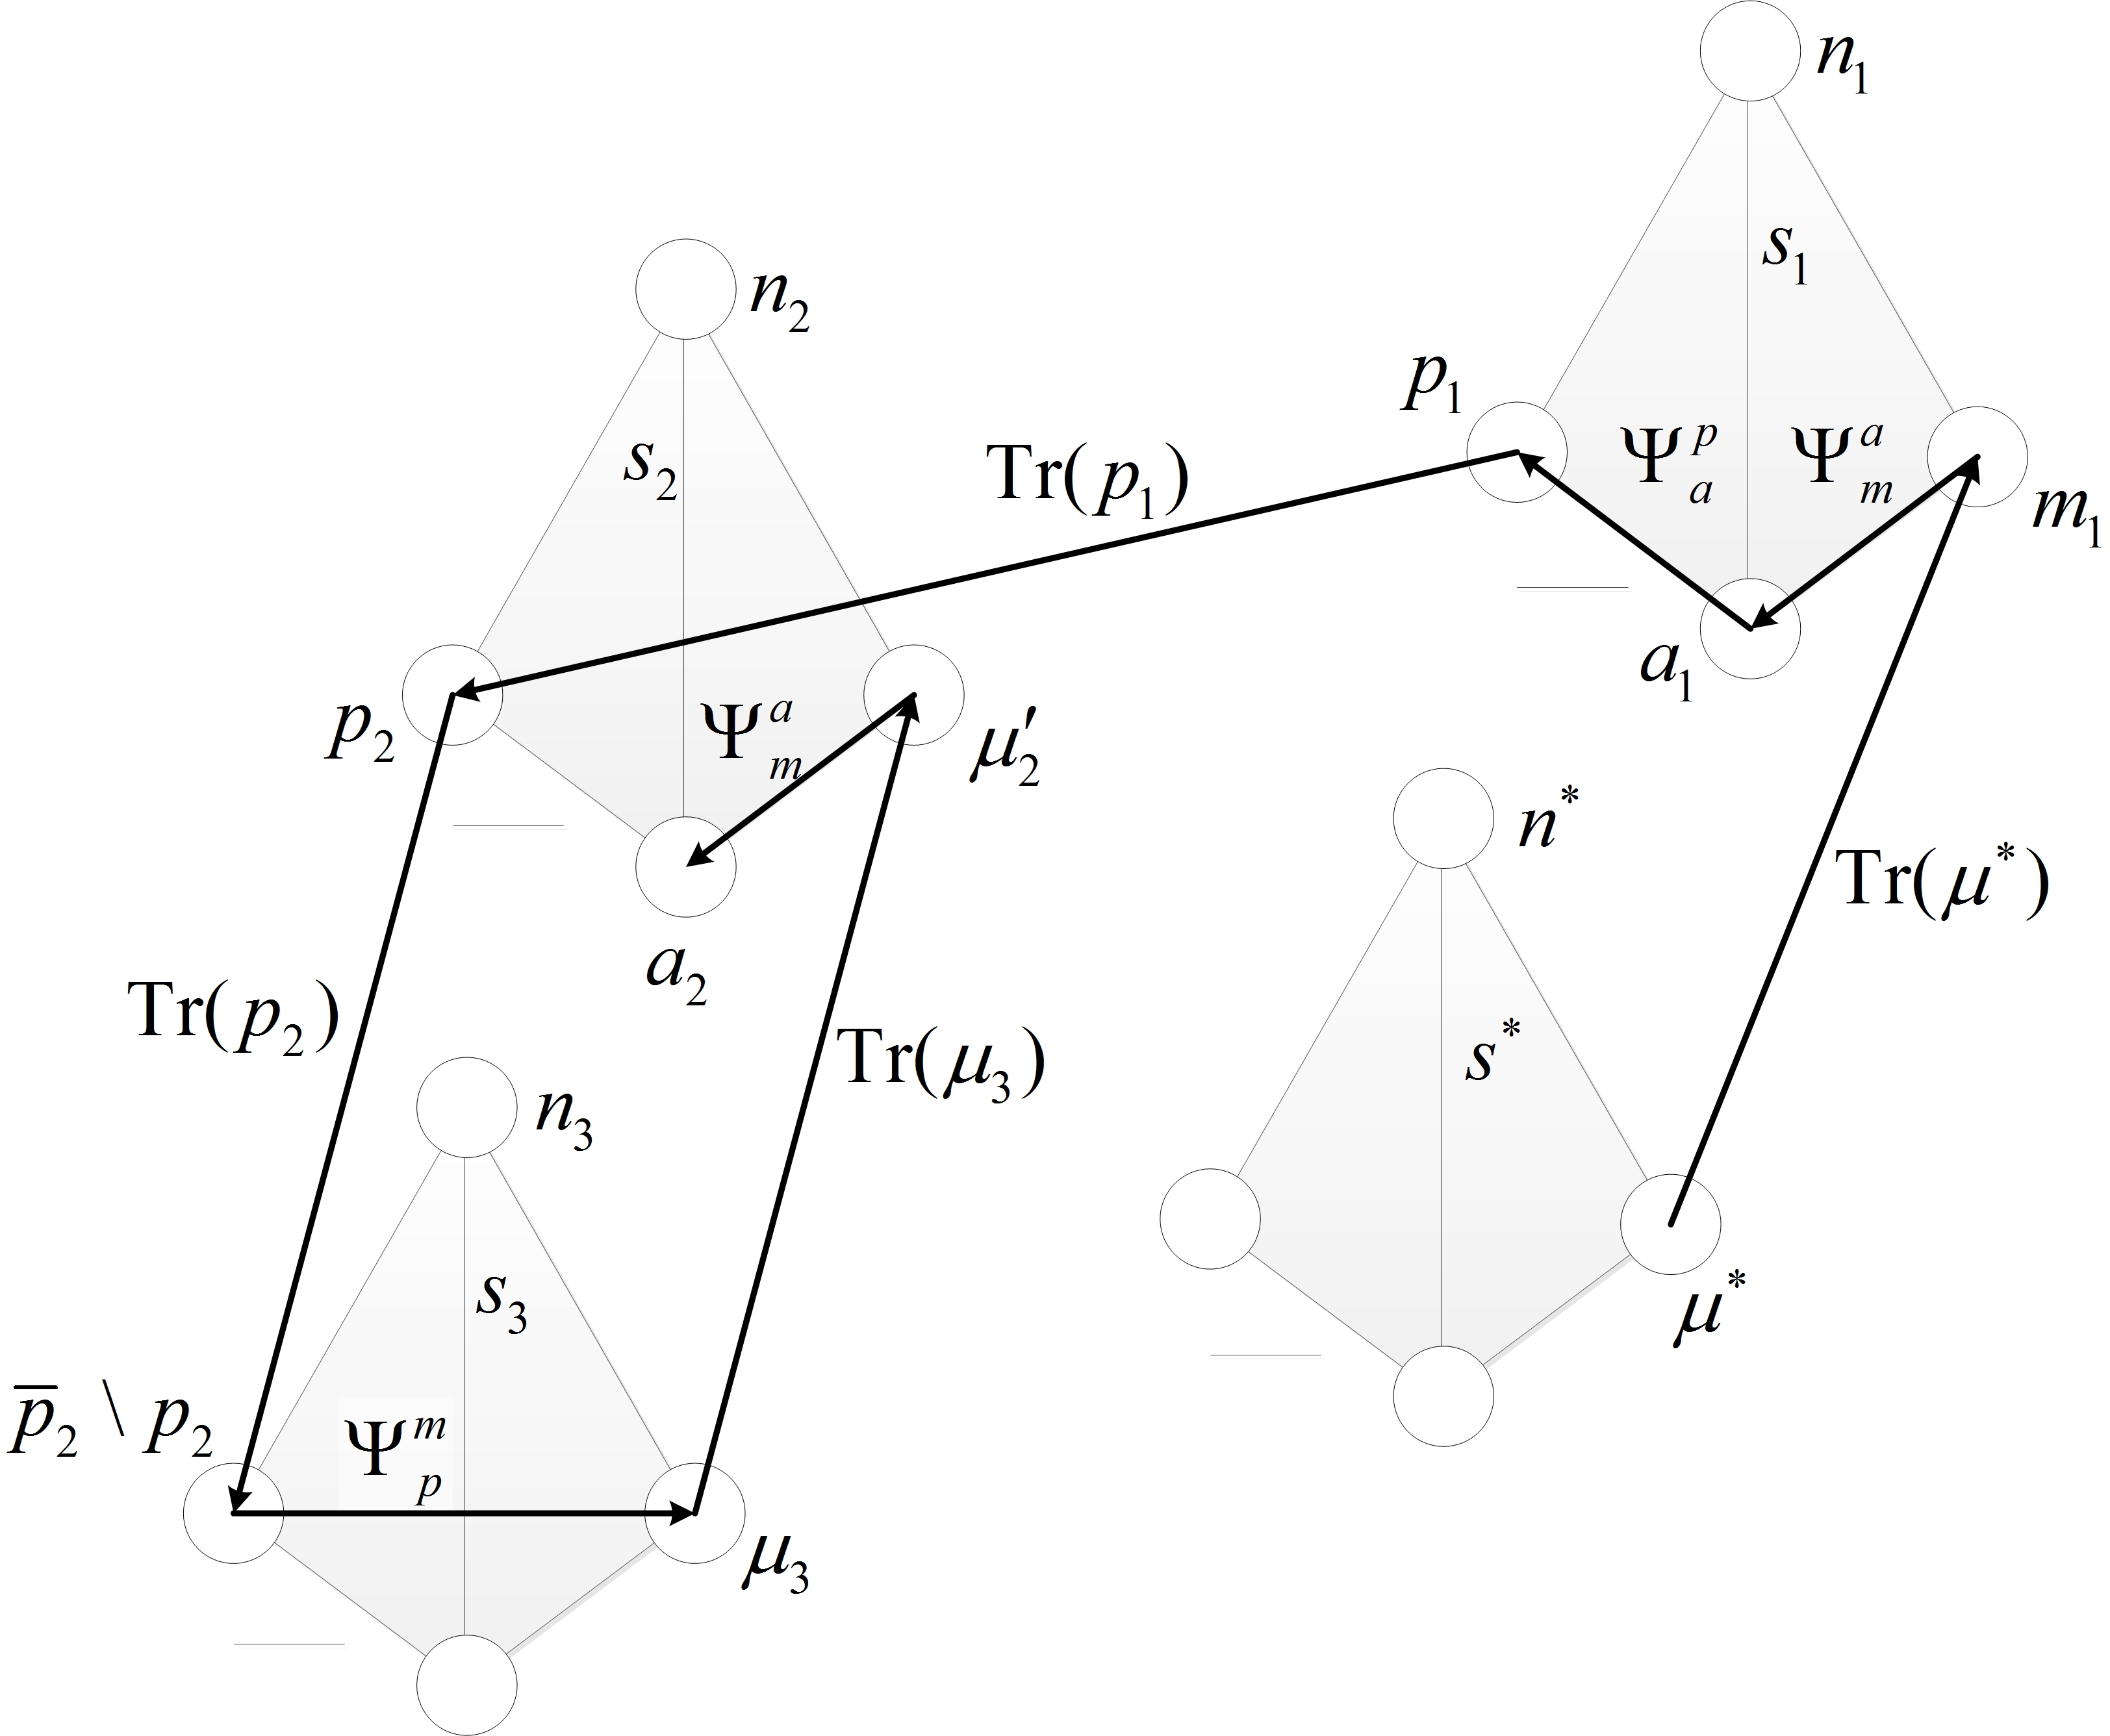
\includegraphics[width=\linewidth]{goalsetting_alg.jpg}
	\caption[]{Иллюстрация к алгоритму целеполагания: $s^*$ "--- знак предмета потребности, $\mu^*$ "--- экземпляр его значения, иначе говоря, мотив деятельности. Стрелками обозначены операторы $\Psi_p^m$, $\Psi_m^a$, $\Psi_a^p$ и $Tr$.}
	\label{fg:goalsetting_alg}
\end{figure}

\textbf{Пример}. Опишем в качестве простого примера процедуру целеполагания руководителя команды разработчиков программного обеспечения (Рисунке~\ref{fg:goalsetting_ex}).

\begin{figure}[h]
	\centering
	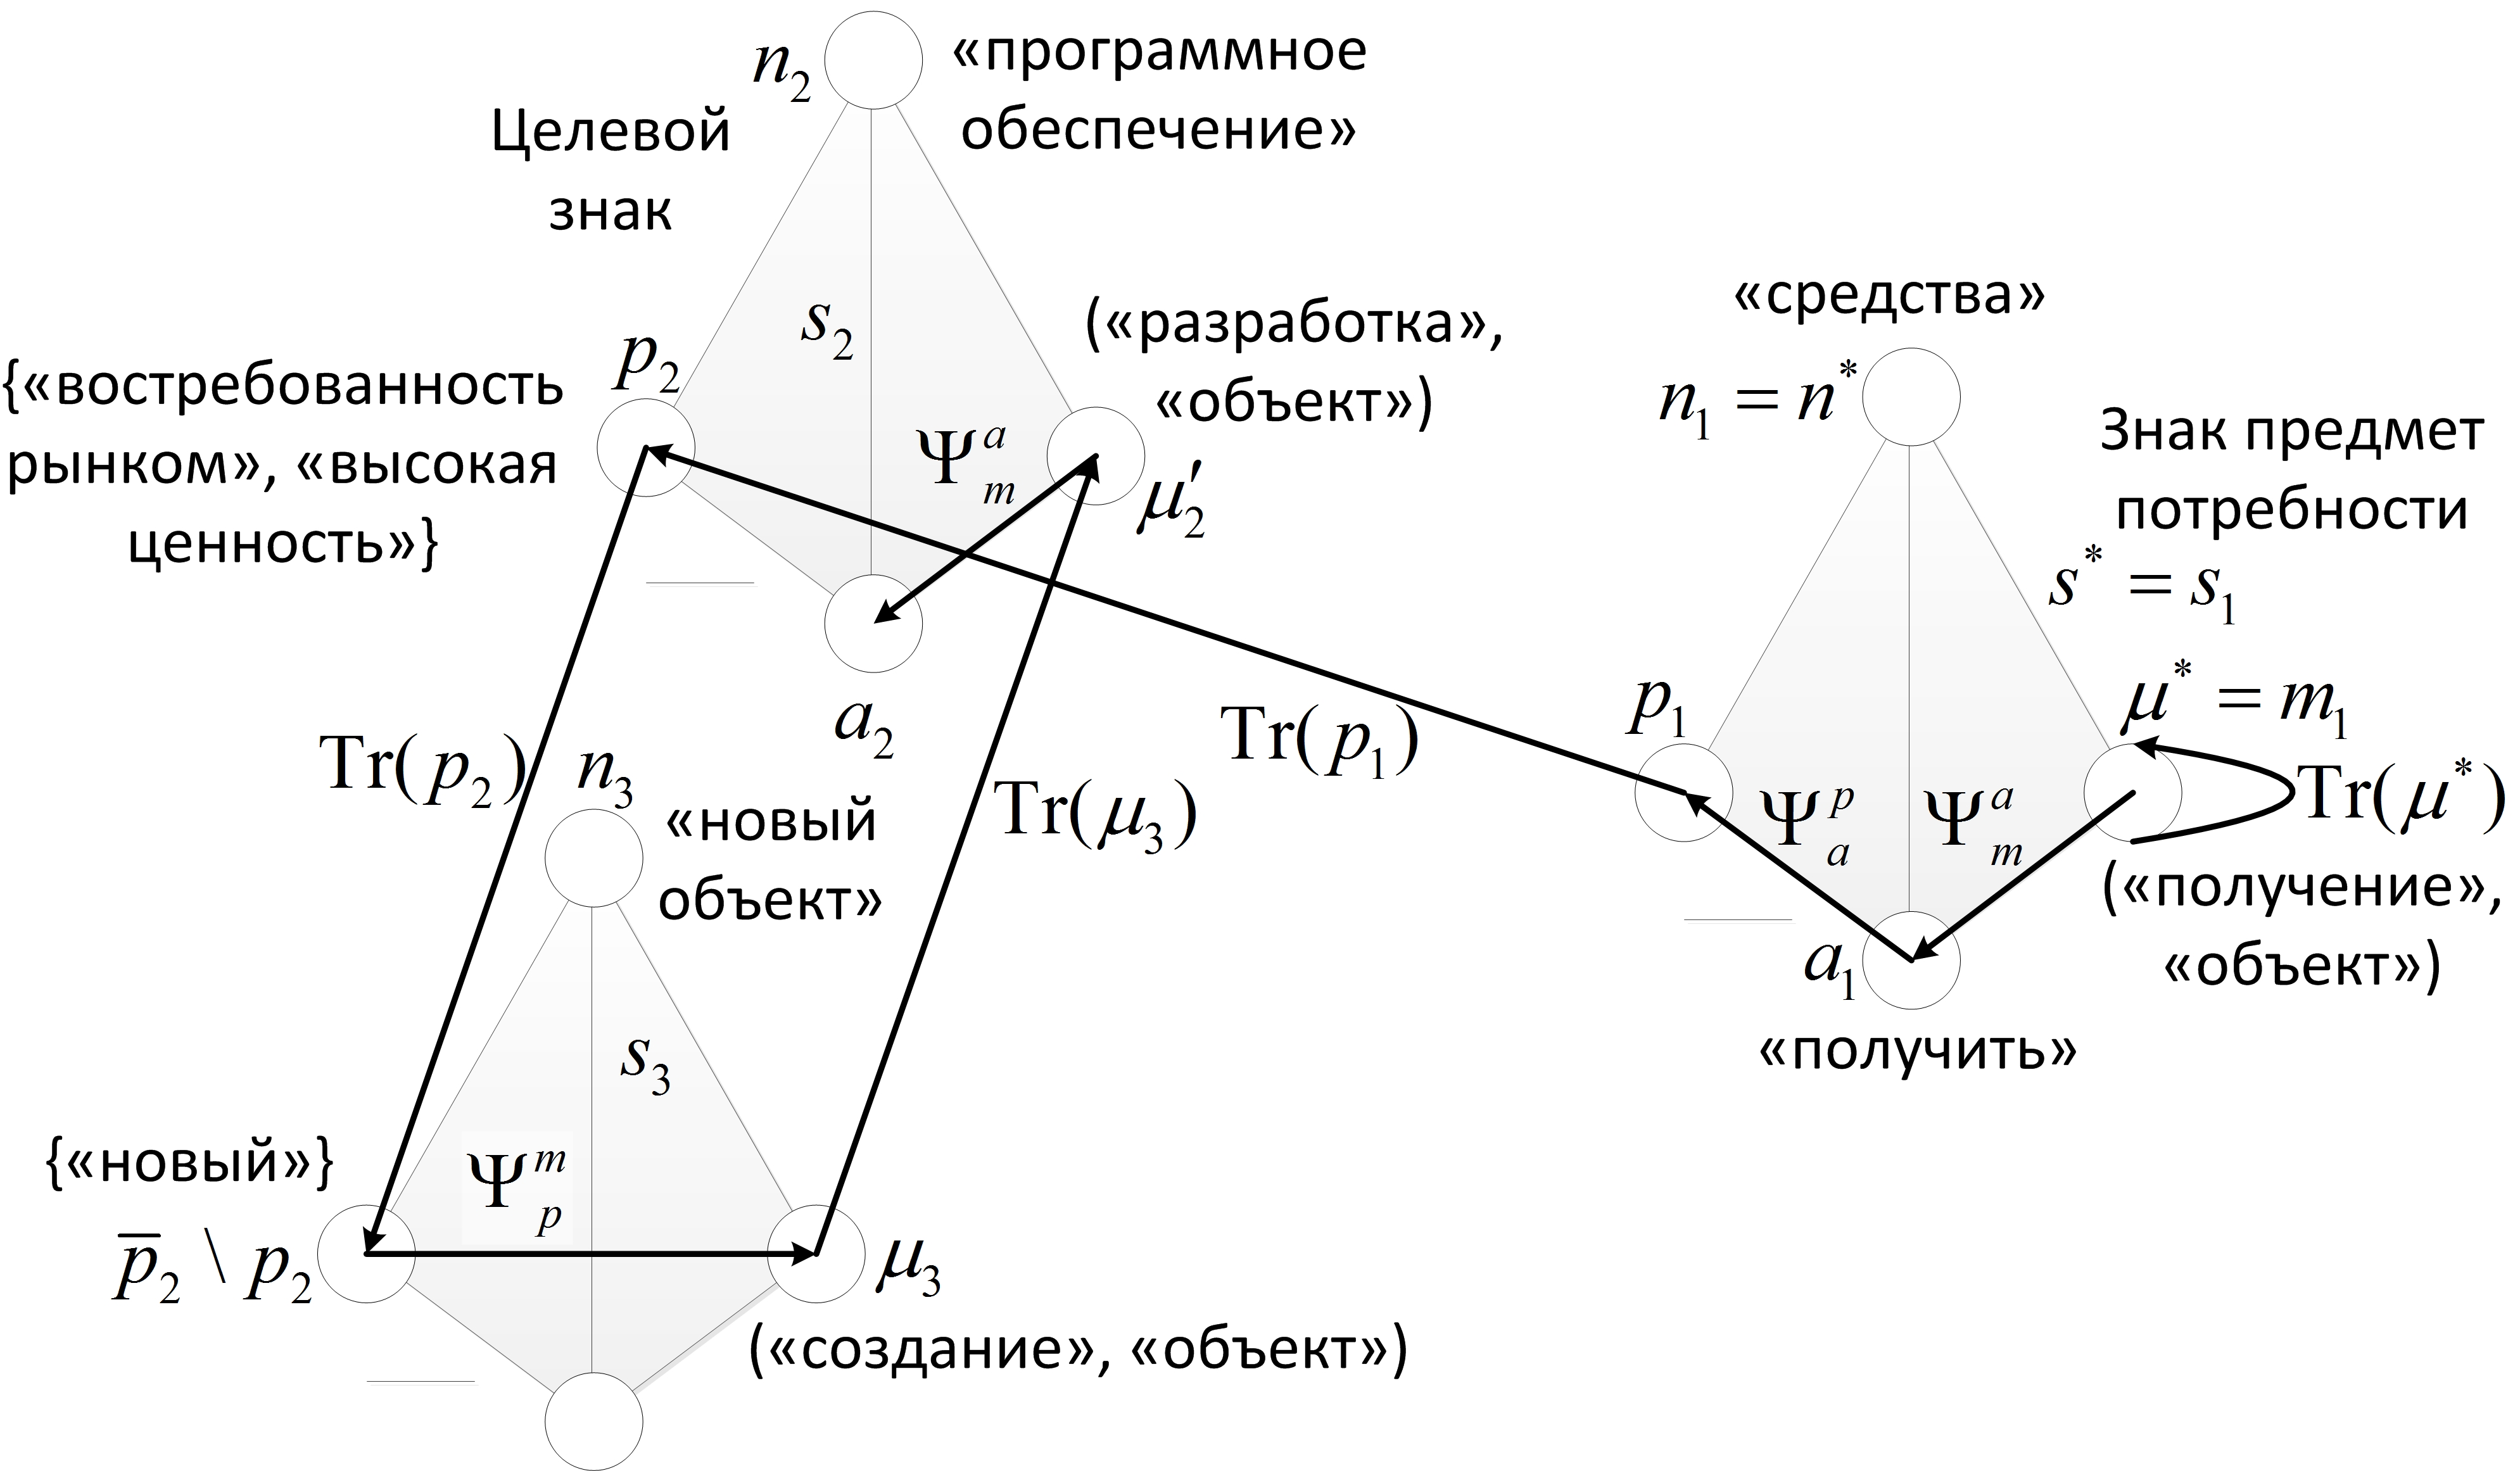
\includegraphics[width=\linewidth]{goalsetting_ex.jpg}
	\caption[]{Пример процесса целеполагания руководителя команды разработчиков с житейской картиной мира. Знаком предмета потребности руководителя является знак с именем <<средства>>. Стрелками обозначены операторы $\Psi_p^m$, $\Psi_m^a$, $\Psi_a^p$ и $Tr$.}
	\label{fg:goalsetting_ex}
\end{figure}

Руководитель команды использует в данном случае житейскую картину мира, мотивом его деятельности является значение знака <<средства>>, один из экземпляров значения которого "--- <<получение>>, обладающее семантической валентностью <<объект>>. Иначе говоря, один из экземпляров значений знака средства есть пара (<<получение>>, <<объект>>). Предположим, образ этого знака содержит признаки: <<высокая ценность>>, <<востребованность рынком>>, <<новое>>.

\textbf{Алгоритм GS.}

\textbf{Вход}: знак <<средства>> и мотив (<<получение>>, <<объект>>).

\textbf{Шаг 1}: переход значение "--- личностный смысл. Сценарий образуется семантическими валентностями предикатного слова, (в данном случае "--- <<получение>>). Субъект ищет знак, при этом его личностный смысл интерпретируется действиями, которые он будет осуществлять, чтобы удовлетворить мотив. Иначе говоря, в множестве добавлений правила, интерпретирующего личностный смысл, должны содержаться необходимые признаки предмета, за который происходит получение средств, например <<высокая ценность>>, <<востребованность рынком>>, <<новое>> и т.д. Предположим, что будет найден личностный смысл <<получить>> знака <<средства>>.

\textbf{Шаг 2}: переход личностный смысл "--- образ. Выполнение действия, соответствующего найденному личностному смыслу, требует удовлетворения признаков из условия действия. Происходит поиск такого знака, образ которого содержит необходимые признаки. Так как руководитель команды разработчиков имеет дело с программным обеспечением, то рано или поздно им будет найден знак <<программное обеспечение>>, так как его образ содержит признаки <<высокая ценность>>, <<востребованность рынком>>. Неудовлетворённые признаки из условия правила вместе с удовлетворёнными образуют расширенный образ, например <<новое программное обеспечение>>.

\textbf{Шаг 3}: переход образ "--- значение. Ищется знак, содержащий в образе признак <<новый>>, например знак <<новый объект>>. Выбираем экземпляр значения этого знака. Экземпляр значения должен быть первым в каком-либо сценарии, совпадающим с каким-либо сценарием знака <<программное обеспечение>>. Таким экземпляром может служить <<создание>>, так как в картине мира руководителя команды имеется необходимый сценарий. Для соответствующего сценария, порождённого знаком <<программное обеспечение>>, первым экземпляром в таком случае выступает <<разработать>>.

\textbf{Шаг 4}: переход значение "--- личностный смысл. Выбирается личностный смысл знака <<программное обеспечение>>, соответствующий экземпляру значения <<разработать>>. Действие, интерпретирующее этот личностный смысл, в множестве добавляемых признаков будет включать признаки <<высокая ценность>>, <<востребованность рынком>>, <<новое>>, содержащиеся в образе знака <<средства>> и удовлетворяющие мотив. Таким образом, текущий знак является целевым, а целью "--- пара <<разработать>> "--- <<программное обеспечение>>.

\textbf{Выход}: знак <<программное обеспечение>> и его личностный смысл <<разработать>>.

\end{document}